% Chapter 5: Code generation using patterns

\chapter{Code generation using patterns}

\label{ch:fifth} % For referencing the chapter elsewhere, use \autoref{ch:name} 
\label{chapter:codeGeneration}

In the previous two chapters we discussed how regular parallel pattern, referred to as \emph{algorithmic skeletons}, help to simplify programming of modern parallel systems.
Parallel programming of multi-\GPU systems is considerably simplified without sacrificing performance as shown by the evaluation in \autoref{chapter:skelcl-evaluation}.

In this chapter, we address the second main challenge identified in \autoref{chapter:background}: \emph{Performance portability}.
We will present a novel approach for generating efficient and hardware-specific code from compositions of algorithmic skeletons and similar high-level \emph{patterns}.
This systematic, rule-based approach provides performance portability across different types of modern parallel processors. 
In the following \autoref{chapter:codeGeneration-evaluation} we will use a set of example applications to show that our approach generates code matching the performance of highly tuned implementations on \CPUs and \GPUs.

We will start this chapter by looking at optimizations in \OpenCL and how applying them changes the source code of applications.
We will show that these optimizations are often hardware-specific thus breaking portability: optimizations for one particular hardware architecture can lead to poor performance on other hardware architectures.
This will motivate the necessity, when aiming for performance portability, for generating optimized and specialized code from a pattern-based high-level representation.
We will discuss the benefits this code generation approach offers over a library-based approach like \SkelCL presented in \autoref{chapter:skelcl}.
Then we will give an overview of our approach and present it in more detail in the following sections.
\autoref{chapter:codeGeneration-evaluation} will present an evaluation of the approach using a set of application studies.

\newpage

\section{A Case Study of OpenCL Optimizations}
\label{sec:reduce:case-study}
\label{section:reduce:case-study}
To understand the problems of performance and portability in the context of modern parallel processors, we will study a simple application example: parallel reduction.
This discussion is based on the presentation \emph{``Optimizing Parallel Reduction in CUDA''} by \citeauthor{Harris2007}~\cite{Harris2007} where optimizations for implementing parallel reduction using \CUDA and targeting Nvidia \GPUs are presented.
Optimization guidelines like this exist from almost every hardware vendor giving developers advice on how to most efficiently exploit their hardware~\cite{CUDAProgrammingGuide,AMDProgrammingGuide,IntelGPUProgrammingGuide,IntelXeonProgrammingGuide}.

In \autoref{chapter:skelcl} we saw that we can express a parallel reduction using a single algorithmic skeleton: \reduce.
Here we look at how efficient \OpenCL implementations of this algorithm or, more precisely, the parallel summation of an array, look like.
We are especially interested in gradually optimizing this application to see how beneficial the single optimization steps are and how they change the source code.

We will first start by looking at the implementation and optimizations on one particular hardware architecture, using a Nvidia \GPU as our example.
Then we will see how the optimized implementations perform on an AMD \GPU and Intel \CPU, to evaluate their portability.
Finally, we will use our observations to motivate the need for a pattern-based code generator for achieving performance portability.

\subsection{Optimizing Parallel Reduction for Nvidia \GPUs}
For implementing the parallel summation of an array, we study an approach using two \OpenCL kernels.
We start with the elements to be reduced in the leafs of the reduction tree shown in \autoref{fig:reduce:tree}.
The first \OpenCL kernel is executed in parallel by multiple \OpenCL work-groups, four work-groups in the example shown in \autoref{fig:reduce:tree}.
Each work-group produces a temporary result, then the second \OpenCL kernel is executed by a single \OpenCL work-group producing the final result.
This strategy is applied as global synchronization, \ie, synchronization across work-groups, is prohibited inside a single \OpenCL kernel, but the parallel tree-based reduction requires synchronization at each level of the reduction tree.
An implementation with a single \OpenCL kernel would, therefore, be restricted to launch a single \OpenCL work-group and, thus, limit the exploited parallelism.

By using the two-kernel approach, massive parallelism can be exploited in the first phase as multiple work-groups operate concurrently on independent parts of the input array.
The second kernel is launched with a single work-group using synchronization inside the work-group to compute the final result.
The vast majority of the work is done in the first phase and the input size to the second phase is comparable small, therefore, the limited exploitation of parallelism in the second phase does not effect overall performance much.

  \todo{Mare bigger. Include (+), synchronization points, ...}
\begin{figure}[t]
  \centering
  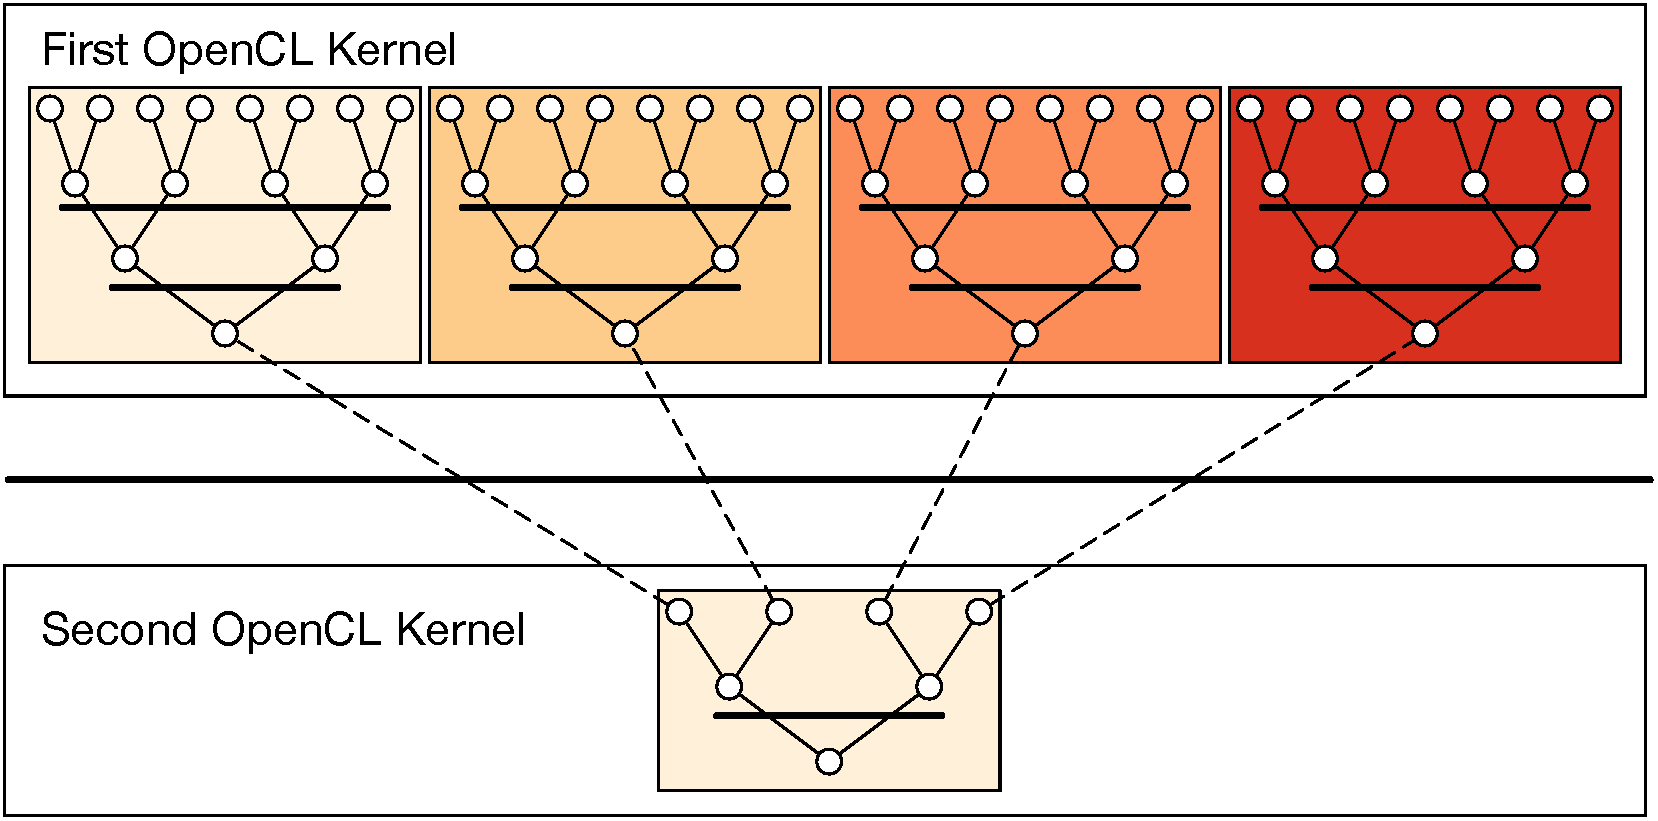
\includegraphics[width=.95\linewidth]{ReduceTree}
  \caption[Parallel Reduction in \OpenCL.]%
    {The first \OpenCL kernel is executed by four work-groups in parallel:
    \ \protect\firstBox{}\,\,work-group $0$,\ \protect\secondBox{}\,\,work-group $1$,\ \protect\thirdBox{}\,\,work-group $2$, \protect\fourthBox{}\,\,work-group $3$.
           The second \OpenCL kernel is only executed by the first work-group.}
  \label{fig:reduce:tree}
\end{figure}

We will follow the methodology in~\cite{Harris2007} and evaluate the performance of the different versions using the measured \GPU memory bandwidth as our metric.
This is reasonable as the reduction has a very low arithmetic intensity and its performance is, therefore, bound by the available \GPU memory bandwidth.
By investigating the memory bandwidth of the \GPU memory, we can see which fraction of the maximum memory bandwidth available has been utilized.

All following implementations are provided by Nvidia as part of their software development kit and presented in~\cite{Harris2007}.
These implementations have originally been developed for Nvidia's Tesla \GPU architecture~\cite{LindholmNOM2008} and not been updated by Nvidia for more recent \GPU architectures.
Nevertheless, the optimizations discussed are still valid on more modern Nvidia \GPUs -- as we will see.
All performance numbers in this section have been measured on a Nvidia GTX 480 \GPU featuring the Nvidia Fermi architecture~\cite{CUDAFermi2009}.

\newpage

\paragraph{First \OpenCL implementation}
\autoref{lst:reduce0} shows the first version of the parallel reduction in \OpenCL.
%
\begin{lstlisting}[%
caption={[First \OpenCL implementation of the parallel reduction.]%
         First \OpenCL implementation of the parallel reduction achieving 6.64\% of the memory bandwith limit.},%
numbers=left,%
float=tb,
label={lst:reduce0}]
kernel
void reduce0(global float* g_idata, global float* g_odata,
             unsigned int n, local float* l_data) {
  unsigned int tid = get_local_id(0);
  unsigned int i   = get_global_id(0);
  l_data[tid] = (i < n) ? g_idata[i] : 0;$\label{lst:reduce0:load}$
  barrier(CLK_LOCAL_MEM_FENCE);$\label{lst:reduce0:firstBarrier}$
  // do reduction in local memory
  for(unsigned int s=1; s < get_local_size(0); s *= 2) {$\label{lst:reduce0:for:start}$
    if ((tid % (2*s)) == 0) {$\label{lst:reduce0:if}$
      l_data[tid] += l_data[tid + s]; }
    barrier(CLK_LOCAL_MEM_FENCE); }$\label{lst:reduce0:for:end}$
  // write result for this work-group to global memory
  if (tid == 0) g_odata[get_group_id(0)] = l_data[0]; }$\label{lst:reduce0:writeBack}$
\end{lstlisting}
% This will be our starting point for the following optimizations.
First each work-item loads an element into the local memory (line~\ref{lst:reduce0:load}).
After a synchronization (line~\ref{lst:reduce0:firstBarrier}) all work-items of a work-group execute a for loop (lines~\ref{lst:reduce0:for:start}--\ref{lst:reduce0:for:end}) to perform a collective tree-based reduction.
In every iteration the if statement (line~\ref{lst:reduce0:if}) ensures that a declining number of work-items remain active performing partial reductions in the shrinking reduction tree.
The second barrier in line~\ref{lst:reduce0:for:end} ensures that no race conditions occur when accessing the shared local memory.
Finally, the work-item in the work-group with id$=0$ writes back the computed result to the global memory in line~\ref{lst:reduce0:writeBack}.


The implementation presented in \autoref{lst:reduce0} is not straightforward to develop.
The application developer has to be familiar with the parallel execution model of \OpenCL to avoid race conditions and deadlocks.
For example, it is important that the second barrier in line~\ref{lst:reduce0:for:end} is placed \emph{after} and not \emph{inside} the if statement.
This is true, even though work-items not entering the if statement will never read from or write to memory and, therefore, can never be influenced by a race condition.
Nevertheless, \OpenCL requires all work-items of a work-group to execute all barrier statements in a kernel exactly the same number of times.
The application developer is responsible to ensure that this condition is met, otherwise a deadlock will occur.

Despite being difficult to program, this implementation does not provide high performance either.
Only 6.64\% of the available bandwidth is utilized.

\begin{lstlisting}[%
caption={[\OpenCL implementation of the parallel reduction avoiding divergent branching.]%
         \OpenCL implementation of the parallel reduction avoiding divergent branching.
         This implementation utilizes 9.73\% of the memory bandwidth limit.},%
numbers=left,%
float=tb,
label={lst:reduce1}]
kernel
void reduce1(global float* g_idata, global float* g_odata,
             unsigned int n, local float* l_data) {
  unsigned int tid = get_local_id(0);
  unsigned int i   = get_global_id(0);
  l_data[tid] = (i < n) ? g_idata[i] : 0;
  barrier(CLK_LOCAL_MEM_FENCE);

  for(unsigned int s=1; s < get_local_size(0); s *= 2) {
      // continuous work-items remain active
      $\strut$@int index = 2 * s * tid;@$\label{lst:reduce1:index}$
      if (@index < get_local_size(0)@) {$\label{lst:reduce1:if}$
          l_data[index] += l_data[index + s]; }$\label{lst:reduce1:read}$
      barrier(CLK_LOCAL_MEM_FENCE); }

  if (tid == 0) g_odata[get_group_id(0)] = l_data[0]; }
\end{lstlisting}

\paragraph{Avoid divergent branching}

\autoref{lst:reduce1} shows the second implementation.
The differences from the previous implementation are highlighted in the code.

When performing the collective tree-based reduction in a work-group, a shrinking number of work-items remain active until the last remaining work-item computes the result of the entire work-group.
In the previous version the modulo operator was used to determine which work-item remains active (see line~\ref{lst:reduce0:if} in \autoref{lst:reduce0}).
This leads to a situation were not the consecutive work-items remain active, but rather work-items which id is divisible by 2, then by 4, then by 8, and so on.
In Nvidia's \GPU architectures, 32 work-items are grouped into a \emph{warp} and executed together, as described in \autoref{chapter:background}.
It is highly beneficial to program in a style where all 32 work-items grouped into a warp perform the same instructions, especially, to avoid divergent branching between work-items of a warp.
Using the modulo operator to determine the active work-items leads to highly divergent branching.
The second implementation in \autoref{lst:reduce1}, therefore, uses a different formula (line~\ref{lst:reduce1:index}) for determining the active work-items, which avoids divergent branching.

The performance improves by a factor of 2.33 as compared to the first implementation.
However, still only 9.73\% of the theoretically available memory bandwidth are used by this version.


\FloatBarrier
\begin{lstlisting}[%
caption={[\OpenCL implementation of the parallel reduction avoiding local memory bank conflicts.]%
         \OpenCL implementation of the parallel reduction avoiding local memory bank conflicts.
         This implementation utilizes 12.61\% of the memory bandwidth limit.},%
numbers=left,%
float=tb,
label={lst:reduce2}]
kernel
void reduce2(global float* g_idata, global float* g_odata,
             unsigned int n, local float* l_data) {
  unsigned int tid = get_local_id(0);
  unsigned int i   = get_global_id(0);
  l_data[tid] = (i < n) ? g_idata[i] : 0;
  barrier(CLK_LOCAL_MEM_FENCE);

  // process elements in different order
  // requires commutativity!
  for(@unsigned int s=get_local_size(0)/2; s>0; s>>=1@) {$\label{lst:reduce2:s}$
      if (@tid < s@) {
          l_data[@tid@] += l_data[@tid@ + s]; }
      barrier(CLK_LOCAL_MEM_FENCE); }

  if (tid == 0) g_odata[get_group_id(0)] = l_data[0]; }
\end{lstlisting}

\paragraph{Avoid interleaved addressing}

\autoref{lst:reduce2} shows the third implementation.
The differences from the previous implementation are highlighted in the code.

On modern \GPUs the fast local memory is organized in multiple \emph{banks}.
When two, or more, work-items simultaneously access memory locations in the same bank a \emph{bank conflict} occurs which means that all memory requests are processed sequentially and not in parallel as usual.
This is described in more detail in~\autoref{chapter:background}.
The previous two implementations use an access pattern for the local memory which makes bank conflicts likely.
% When reading memory from the local memory in line~\ref{lst:reduce1:read} of \autoref{lst:reduce1} each work-item reads interleaved from two locations: \lstinline!index! and \lstinline!index+s!.
The third implementation in \autoref{lst:reduce2} avoids this problematic local memory access pattern.
Instead an access pattern is used where bank conflicts are unlikely and, thus, performance is improved.
% This is achieved by directly using the local id as index together with a different definition of \lstinline!s! in line~\ref{lst:reduce2:s}.
This better access pattern requires the reduction operation to be commutative, as the order of element is not respected when reading from global memory.

The performance improves by a factor of 2.01 as compared to the previous implementation and 4.68 to the initial implementation.
With this version 12.61\% of the theoretically available memory bandwidth are used.



\FloatBarrier
\newpage

\paragraph{Increase computational intensity per work-item}

\autoref{lst:reduce3} shows the fourth implementation.
The differences from the previous implementation are highlighted in the code.
\begin{lstlisting}[%
caption={[\OpenCL implementation of the parallel reduction. Each work-item performs an addition when loading data from global memory.]%
         \OpenCL implementation of the parallel reduction. Each work-item performs an addition when loading data from global memory.
         This implementation utilizes 23.71\% of the memory bandwidth limit.},%
numbers=left,%
float=tb,
escapechar=\`,
label={lst:reduce3}]
kernel
void reduce3(global float* g_idata, global float* g_odata,
             unsigned int n, local float* l_data) {
  unsigned int tid = get_local_id(0);
  $\strut$@unsigned int i = get_group_id(0) * (get_local_size(0)*2)@
                                   $\strut$@+ get_local_id(0);@
  l_data[tid] = (i < n) ? g_idata[i] : 0;
  // performs first addition during loading
  $\strut$@if (i + get_local_size(0) < n)@
  $\strut$@    l_data[tid] += g_idata[i+get_local_size(0)];@$\label{lst:reduce3:comp}$
  barrier(CLK_LOCAL_MEM_FENCE);

  for(unsigned int s=get_local_size(0)/2; s>0; s>>=1) {
      if (tid < s) {
          l_data[tid] += l_data[tid + s]; }
      barrier(CLK_LOCAL_MEM_FENCE); }

  if (tid == 0) g_odata[get_group_id(0)] = l_data[0]; }
\end{lstlisting}

In the previous versions, each work-item loads one element from the global into local memory before the work-items of the work-group collectively performa tree-based reduction.
That means that half of the work-items are idle after performing a single copy operation, which is highly wasteful.
The fourth implementation in \autoref{lst:reduce3} avoids this by letting each work-item load two elements from global memory, perform an addition, and store the computed result in local memory (line~\ref{lst:reduce3:comp}).
Assuming the same input size this reduces the number of work-items to start by half and, therefore, increases the computational intensity for every work-item.

The performance improves by a factor of 1.78 as compared to the previous implementation and 8.34 to the initial implementation.
With this version, 23.71\% of the theoretically available memory bandwidth is used.



\FloatBarrier
\newpage
\paragraph{Avoid synchronization inside a warp}

\autoref{lst:reduce4} shows the fifth implementation.
The differences from the previous implementation are highlighted in the code.

Wraps are the fundamental execution unit in Nvidia's \GPU architectures, as explained in \autoref{chapter:background}:
32 work-items are grouped together to form a warp based on their id, \ie, work-items with id 0 -- 31 are grouped into the first warp, work-items with id 32 -- 63 into the second warp, and so on.
All work-items grouped in a warp are guaranteed to be executed together in a lock-step manner, \ie, all work-items in the same warp execute the same instruction simultaneously.
Because of this hardware behaviour, no barrier synchronization is required between instructions inside a single warp.
The fifth implementation in \autoref{lst:reduce4} takes advantage of this.
The for loop performing the tree-based reduction is exited early at the stage when only 32 work-items remain active (see line~\ref{lst:reduce4:for}).
Lines~\ref{lst:reduce4:warp:start}--\ref{lst:reduce4:warp:end} shows the special code which performs the rest of the tree-base reduction without any barrier synchronization.
The code shown here effectively unrolled the last six iterations of the for loop in line~\ref{lst:reduce4:for}.
As warps are specific to Nvidia's \GPU architectures, this implementation is not a portable \OpenCL code and might produce incorrect results on other \OpenCL devices.

The performance improves by a factor of 1.8 as compared to the previous implementation and 15.01 to the initial implementation.
With this version, 32.59\% of the theoretically available memory bandwidth is used.

\begin{lstlisting}[%
caption={
         [\OpenCL implementation of the parallel reduction.
         Synchronization inside a warp is avoided by unrolling the loop for the last 32 work-items.]
         \OpenCL implementation of the parallel reduction.
         Synchronization inside a warp is avoided by unrolling the loop for the last 32 work-items.
         This implementation utilizes 32.59\% of the memory bandwidth limit.},%
numbers=left,%
float=p,
label={lst:reduce4}]
kernel
void reduce4(global float* g_idata, global float* g_odata,
             unsigned int n,local volatile float* l_data){
  unsigned int tid = get_local_id(0);
  unsigned int i = get_group_id(0) * (get_local_size(0)*2)
                                   + get_local_id(0);
  l_data[tid] = (i < n) ? g_idata[i] : 0;
  if (i + get_local_size(0) < n)
      l_data[tid] += g_idata[i+get_local_size(0)];
  barrier(CLK_LOCAL_MEM_FENCE);

  // prevent further unrolling (see next version)
  $\strut$@#pragma unroll 1@$\label{lst:reduce4:pragma}$
  for(unsigned int s=get_local_size(0)/2; s>@32@; s>>=1) {$\label{lst:reduce4:for}$
      if (tid < s) {
          l_data[tid] += l_data[tid + s]; }
      barrier(CLK_LOCAL_MEM_FENCE); }

  // unroll for last 32 active work-items
  // no synchronization required on NVIDIA GPUs
  // this is not protable OpenCL code!
  $\strut$@if (tid < 32) {@$\label{lst:reduce4:warp:start}$
  $\strut$@  if (WG_SIZE >= 64) { l_data[tid] += l_data[tid+32]; }@
  $\strut$@  if (WG_SIZE >= 32) { l_data[tid] += l_data[tid+16]; }@
  $\strut$@  if (WG_SIZE >= 16) { l_data[tid] += l_data[tid+ 8]; }@
  $\strut$@  if (WG_SIZE >=  8) { l_data[tid] += l_data[tid+ 4]; }@
  $\strut$@  if (WG_SIZE >=  4) { l_data[tid] += l_data[tid+ 2]; }@
  $\strut$@  if (WG_SIZE >=  2) { l_data[tid] += l_data[tid+ 1]; } }@$\label{lst:reduce4:warp:end}$

  if (tid == 0) g_odata[get_group_id(0)] = l_data[0]; }
\end{lstlisting}

\paragraph{Complete loop unrolling}

\autoref{lst:reduce5} on page~\pageref{lst:reduce5} shows the sixth implementation.
The differences from the previous implementation are highlighted in the code.

In the previous implementation we made a special case for the last six iterations of the for loop and provided special code handling for each iteration separately.
This is a general optimization strategy known as \emph{loop unrolling}.
Loop unrolling can be beneficial because variables and branches required by a loop can be avoided.
In the sixth implementation, shown in \autoref{lst:reduce5}, the for loop has been removed entirely and replaced by three if statement (line~\ref{lst:reduce5:if:1},~\ref{lst:reduce5:if:2}, and~\ref{lst:reduce5:if:3}).
Each if statement replaces one iteration of the loop.
This code assumes that \code{WG\_SIZE} is a compile-time constant and, therefore, the if statements will be evaluated at compile time, avoiding costly branches at runtime.
Different to the previous optimization, we still have to provide a barrier to ensure correct synchronization, as multiple warps are involved here.

The performance improves by a factor of 1.41 as compared to the previous implementation and 21.16 to the initial implementation.
With this version, 36.77\% of the theoretically available memory bandwidth are used.

\begin{lstlisting}[%
caption={[\OpenCL implementation of the parallel reduction with a completly unrolled loop.]
         \OpenCL implementation of the parallel reduction with a completly unrolled loop.
         This implementation utilizes 36.77\% of the memory bandwidth limit.},%
numbers=left,%
float=p,
label={lst:reduce5}]
kernel
void reduce5(global float* g_idata, global float* g_odata,
             unsigned int n,local volatile float* l_data){
  unsigned int tid = get_local_id(0);
  unsigned int i = get_group_id(0) * (get_local_size(0)*2)
                                   + get_local_id(0);
  l_data[tid] = (i < n) ? g_idata[i] : 0;
  if (i + get_local_size(0) < n)
      l_data[tid] += g_idata[i+get_local_size(0)];
  barrier(CLK_LOCAL_MEM_FENCE);

  // unroll for loop entirely
  $\strut$@if (WG_SIZE >= 512) {@$\label{lst:reduce5:if:1}$
  $\strut$@    if (tid < 256) { l_data[tid] += l_data[tid+256]; }@
  $\strut$@    barrier(CLK_LOCAL_MEM_FENCE); }@
  $\strut$@if (WG_SIZE >= 256) {@$\label{lst:reduce5:if:2}$
  $\strut$@    if (tid < 128) { l_data[tid] += l_data[tid+128]; }@
  $\strut$@    barrier(CLK_LOCAL_MEM_FENCE); }@
  $\strut$@if (WG_SIZE >= 128) {@$\label{lst:reduce5:if:3}$
  $\strut$@    if (tid <  64) { l_data[tid] += l_data[tid+ 64]; }@
  $\strut$@    barrier(CLK_LOCAL_MEM_FENCE); }@

  if (tid < 32) {
    if (WG_SIZE >= 64) { l_data[tid] += l_data[tid+32]; }
    if (WG_SIZE >= 32) { l_data[tid] += l_data[tid+16]; }
    if (WG_SIZE >= 16) { l_data[tid] += l_data[tid+ 8]; }
    if (WG_SIZE >=  8) { l_data[tid] += l_data[tid+ 4]; }
    if (WG_SIZE >=  4) { l_data[tid] += l_data[tid+ 2]; }
    if (WG_SIZE >=  2) { l_data[tid] += l_data[tid+ 1]; } }

  if (tid == 0) g_odata[get_group_id(0)] = l_data[0]; }
\end{lstlisting}


\paragraph{Fully optimized implementation\hfill\strut}

\autoref{lst:reduce6} on page~\pageref{lst:reduce6} shows the final and fully optimized implementation.
The differences from the previous implementation are highlighted in the code.

One of the optimizations applied earlier was to increase the computational intensity for each single work-item by performing two loads and an addition instead of a single load.
This final version applies the same idea, but performing multiple additions per work-item before the collective tree-based reduction in the entire work-group.
This has indeed two advantages:
first, the algorithmic intensity is increased, \ie, each work-item is doing more work,
and, second, performing the summation sequentially by a single work-item does not require costly synchronizations.
The fully optimized implementation is shown in \autoref{lst:reduce6} with the changes highlighted.
A while loop has been introduced (see line~\ref{lst:reduce6:while}) which, in every iteration, loads two elements from the global memory and adds them to the local memory.
No synchronization is required here as each work-item operates independently on different memory locations.
The way the memory is accessed ensures that memory accesses will be coalesced (see \autoref{chapter:background}) when reading from global memory.

The performance improves by a factor of 1.42 as compared to the previous implementation and 30.04 to the initial implementation.
With this version, 65.44\% of the theoretically available memory bandwidth are used.

\begin{lstlisting}[%
caption={[Fully optimized \OpenCL implementation of the parallel reduction.]
         Fully optimized \OpenCL implementation of the parallel reduction.
         This implementation utilizes 65.44\% of the memory bandwidth limit.},%
numbers=left,%
float=p,
label={lst:reduce6}]
kernel
void reduce6(global float* g_idata, global float* g_odata,
             unsigned int n,local volatile float* l_data){
  unsigned int tid = get_local_id(0);
  unsigned int i = get_group_id(0) * (get_local_size(0)*2)
                                   + get_local_id(0);
  $\strut$@unsigned int gridSize = WG_SIZE*2*get_num_groups(0);@
  $\strut$@l_data[tid] = 0;@

  // multiple elements are reduced per work-item
  $\strut$@while (i < n) { l_data[tid] += g_idata[i];@$\label{lst:reduce6:while}$
  $\strut$@                if (i + WG_SIZE < n)@
  $\strut$@                  l_data[tid] += g_idata[i+WG_SIZE];@
  $\strut$@                i += gridSize; }@
  barrier(CLK_LOCAL_MEM_FENCE);

  if (WG_SIZE >= 512) {
      if (tid < 256) { l_data[tid] += l_data[tid+256]; }
      barrier(CLK_LOCAL_MEM_FENCE); }
  if (WG_SIZE >= 256) {
      if (tid < 128) { l_data[tid] += l_data[tid+128]; }
      barrier(CLK_LOCAL_MEM_FENCE); }
  if (WG_SIZE >= 128) {
      if (tid <  64) { l_data[tid] += l_data[tid+ 64]; }
      barrier(CLK_LOCAL_MEM_FENCE); }

  if (tid < 32) {
    if (WG_SIZE >= 64) { l_data[tid] += l_data[tid+32]; }
    if (WG_SIZE >= 32) { l_data[tid] += l_data[tid+16]; }
    if (WG_SIZE >= 16) { l_data[tid] += l_data[tid+ 8]; }
    if (WG_SIZE >=  8) { l_data[tid] += l_data[tid+ 4]; }
    if (WG_SIZE >=  4) { l_data[tid] += l_data[tid+ 2]; }
    if (WG_SIZE >=  2) { l_data[tid] += l_data[tid+ 1]; } }

  if (tid == 0) g_odata[get_group_id(0)] = l_data[0]; }
\end{lstlisting}


\paragraph{Conclusions\hfill\strut}
We can draw several valuable conclusions from studying these \OpenCL source codes.

The first main conclusion is, that implementing these optimizations is not intuitive and straightforward.
It requires experience as well as knowledge and reasoning about the target hardware architecture, in this case Fermi \GPU architectures:
\autoref{lst:reduce1} requires the understanding of the problem of \emph{branch divergence}, \autoref{lst:reduce2} requires knowledge about the organization of local memory and \emph{bank conflicts}, \autoref{lst:reduce3} and \autoref{lst:reduce6} require reasoning about the \emph{computational intensity} of work-items, \autoref{lst:reduce4} requires understanding of \emph{warps} and their execution by the hardware, \autoref{lst:reduce5} requires experience with \emph{loop unrolling} techniques, and, finally, \autoref{lst:reduce6} required knowledge about the organization of global memory and \emph{memory coalescing}.
The author wants to empathize that these are \emph{additional} burdens for the application developer on top of implementing a functionally correct version facing widely recognized correctness problems of parallel programming like dealing with race conditions and deadlocks.

Furthermore, the source code changes necessary for individual optimization steps are not obvious either.
While the performance increases gradually, the source code changes are more radical.
The source code of the first implementation in \autoref{lst:reduce0} is very different as compared to the final implementation shown in \autoref{lst:reduce6}.
For example, the code size has more then doubled (from 16 to 35 lines of code) and many statements have been added or replaced others.
It is not obvious, neither to a human being nor to an optimizing compiler, that these two pieces of code have the same semantics (assuming an associative and commutative binary reduction operator, \eg, $+$).

The second main conclusion we can draw is, that performing these optimizations on modern parallel architectures is highly beneficial.
The first unoptimized version did only utilize about 6.64\% of the available memory bandwidth, while the fully optimized version utilizes a more reasonable 65.44\% on our GeForce GTX 480.
Applying all optimizations improved the performance by a factor of $\approx${}$10$ while utilizing the exactly same hardware.
For an input array of size of 256 MB the runtime reduces from 95.7 ms to 9.1 ms when using the optimized kernel over the unoptimized one.
Harris~\cite{Harris2007} reports an even higher improvement factor of $\approx${}$30$ for the GeForce 8800 GTX used in his experiments.
Modern parallel processors are often chosen as target architecture because of their high theoretical performance.
Turning the theoretical performance into practical performance by applying such optimizations is, therefore, \emph{essential} for most users.





\subsection{Portability of the Optimized Parallel Reduction}
After we have established how crucial but hard to achieve optimizations are, we now will investigate their portability.
To do so, we run the code shown in \autoref{lst:reduce0}--\ref{lst:reduce6} on three different hardware architectures:
Nvidia's Fermi \GPU architecture~\cite{CUDAFermi2009} which we have used in our analysis in the previous section, AMD's Graphics Core Next \GPU architecture~\cite{AMDGCN2012}, and Intel's Nehalem \CPU architecture~\cite{IntelNehalem2008}.
\autoref{fig:reduce:overview} shows the performance numbers for each architecture.
We use, as before, the memory bandwidth as our performance metric and show the hardware memory bandwidth limit of each respective hardware architecture.
As a practical comparison we also show performance numbers for the parallel reduction using highly tuned, architecture specific implementations of the BLAS library.
We use the cuBLAS library~\cite{cuBLAS} for the Nvidia \GPU, the clBLAS library~\cite{clBLAS} for the AMD \GPU, and the MKL library~\cite{MKL} for the Intel \CPU.
Each of these libraries is implemented and provided by the corresponding hardware vendor.

\begin{figure}[p]
  \centering
\begin{subfigure}{\linewidth}
  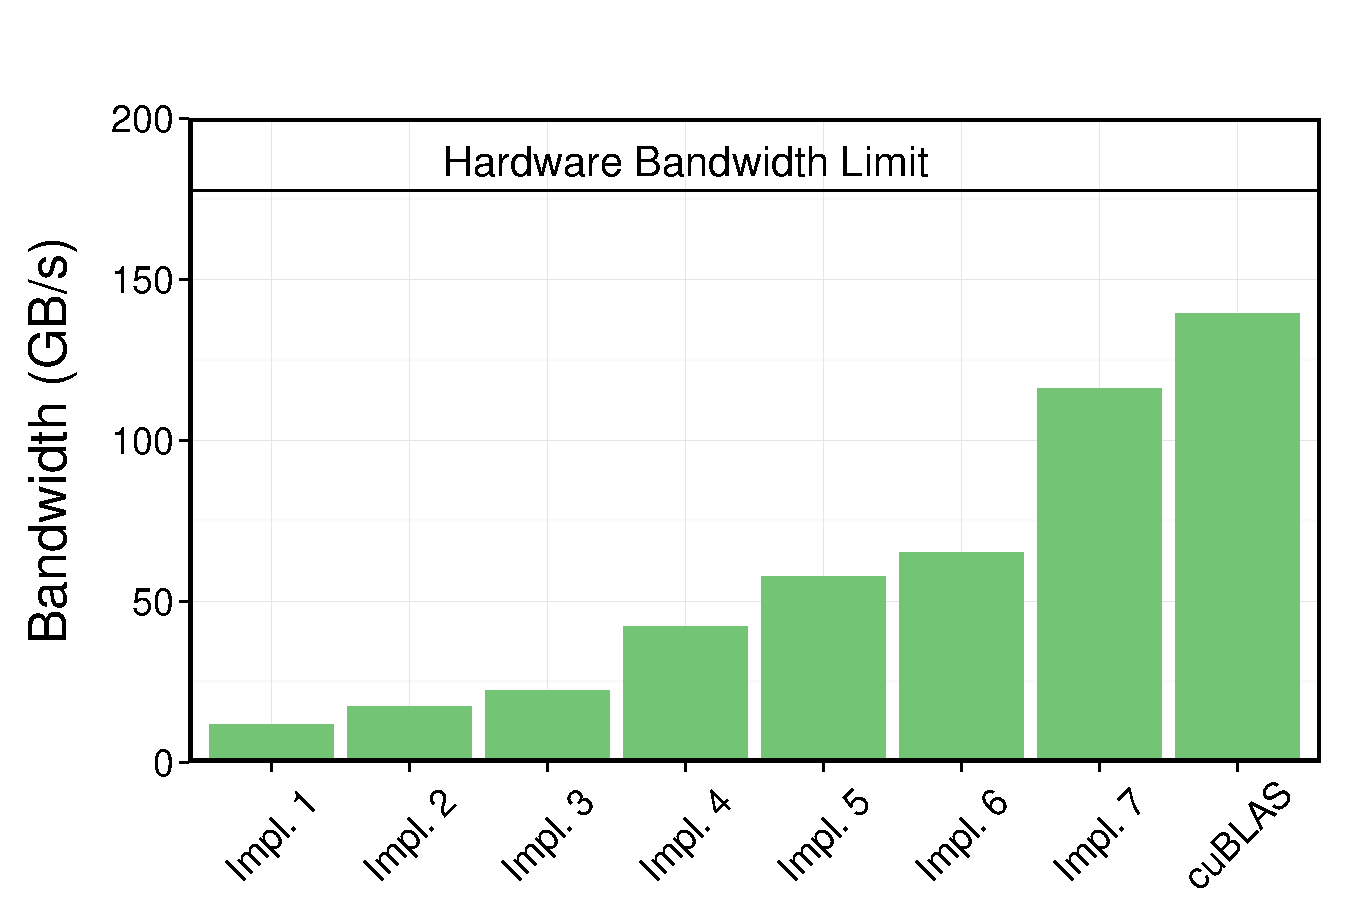
\includegraphics[width=.85\linewidth]{Plots/Reduction/reduce_nv}
  \caption{Nvidia's GTX 480 \GPU.}
  \label{fig:reduce:nvidia}
\end{subfigure}\\
\begin{subfigure}{\linewidth}
  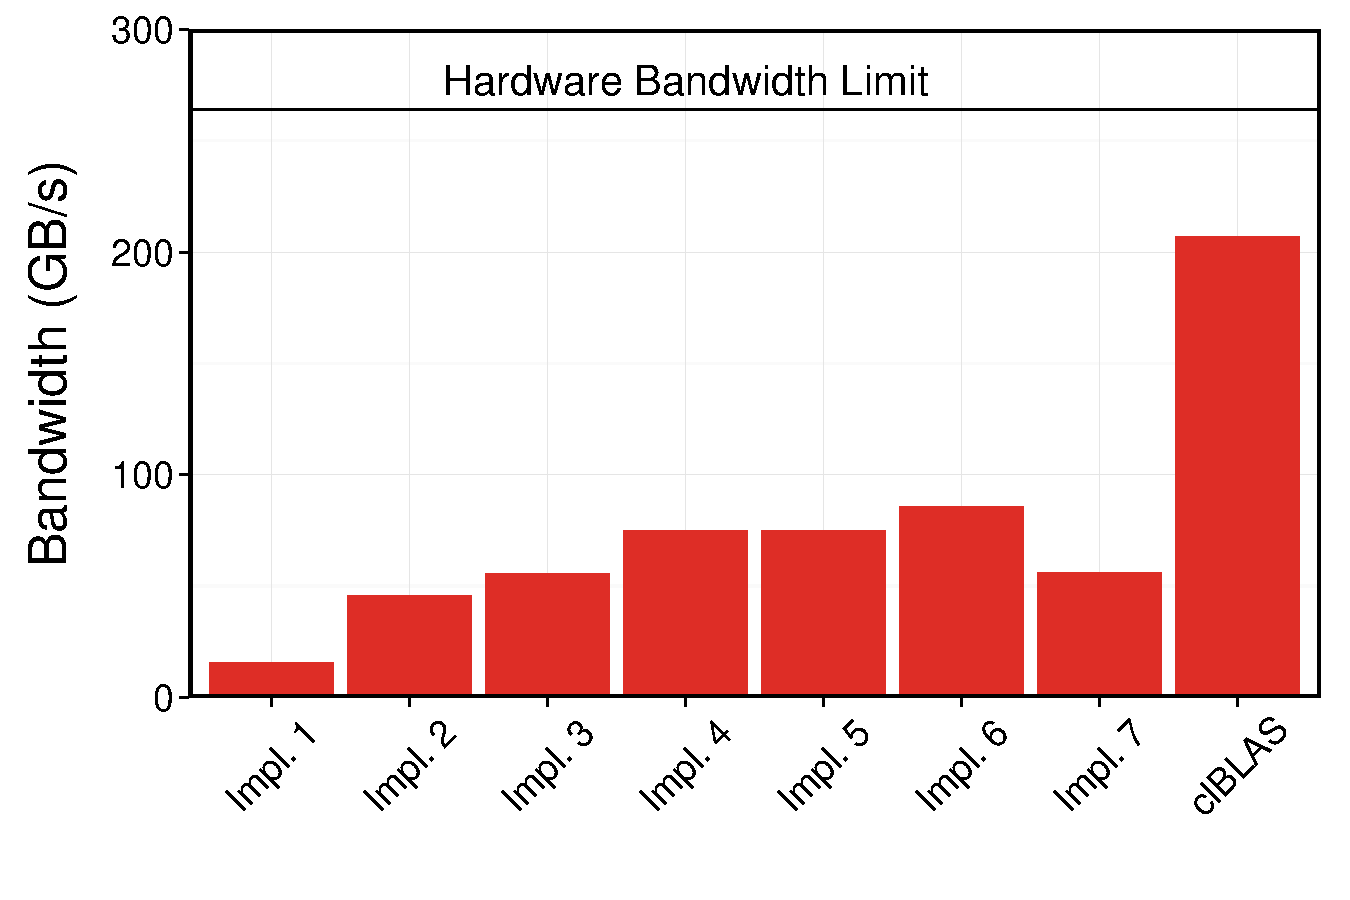
\includegraphics[width=.85\linewidth]{Plots/Reduction/reduce_amd}
  \caption{AMD's HD 7970 \GPU.}
  \label{fig:reduce:amd}
\end{subfigure}\\
\begin{subfigure}{\linewidth}
  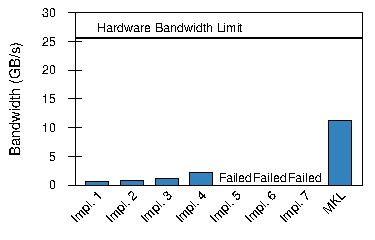
\includegraphics[width=.85\linewidth]{Plots/Reduction/reduce_intel}
    \caption{Intel's E5530 dual-socket \CPU.}
  \label{fig:reduce:intel}
\end{subfigure}
  \caption{Performance of differently optimized implementations of the parallel reduction.}
  \label{fig:reduce:overview}
\end{figure}


\paragraph{Portability of Optimizations}
The results show that the optimizations discussed in the previous section are not portable.
On each architecture a different version of the optimized implementations performs best:
Implementation~7 (shown in \autoref{lst:reduce6}) on the Nvidia \GPU, Implementation~6 (shown in \autoref{lst:reduce5}) on the AMD \GPU, and Implementation~4 (shown in \autoref{lst:reduce3}) on the Intel \CPU.
Some implementations actually produce incorrect results on the Intel \CPU due to the warp-specific optimization introduced in Implementation~5 (shown in \autoref{lst:reduce4}).
Interestingly, this optimization happens to be valid on AMD's \GPU architecture as well, as there exists a similar concept to warps called \emph{wavefronts}~\cite{AMDGCN2012}.

\paragraph{Portability of Relative Performance}
\emph{Relative performance} refers to the performance of an implementation relative to the best theoretical or practical performance possible on the same hardware architecture.
The theoretical performance of an architecture is given by its hardware limitations, like the number of arithmetic logical units, the width of the memory bus, or the maximum clock frequency.
Practical issues like work load and utilization or the cache miss rate are ignored.
Possible metrics for measuring the theoretical performance are number of floating point operation in GFLOP/s or the memory bandwidth in GB/s.

The best practical performance is measured by comparison with the best possible implementation available for a particular hardware platform.
It is not always possible to determine which implementation is the best.
Here we consider the BLAS library implementations tuned by the respective hardware vendors as the best available.

By investigating the relative performance we can compare how well optimizations apply across different hardware architectures.
The \emph{relative performance} achieved differs widely across architectures, as we can see in \autoref{fig:reduce:overview}.

On the Nvidia \GPU, the best optimized implementation achieves 83.3\% of the performance of the vendor-provided cuBLAS implementation and utilizes 65.4\% of the theoretical memory bandwidth limit.

On the AMD \GPU, the gap between the manual and library implementation is much larger:
the manually optimized implementation achieves only 41.3\% of the clBLAS library implementation.
Only 32.4\% of the theoretical memory bandwidth limit is achieved.

On the Intel \CPU, implementation~4 achieves only 16.6\% of the MKL performance.
That means, that MKL is over 5 times faster than the best of the discussed implementations.
The hardware bandwidth limit is only utilized to 8.6\%.
Interestingly, the MKL implementation also only provides 43.8\% of the maximum memory bandwidth.
This is due to the combination of the implementation of the parallel reduction in MKL and the particular machine used in this experiment.
The test machine used is configured as a dual-socket machine, \ie, two E5530 \CPUs each with their own memory controller are available.
Therefore, the hardware bandwidth available is doubled as compared to a single E5530 \CPU.
While the implementation of the parallel reduction in the MKL library is optimized using vector instructions, it does not exploit thread-level parallelism.
Therefore, the second E5530 \CPU can not be used by the implementation, thus, limiting the available bandwidth by a factor of 2.

\paragraph{Conclusions}
Studying the performance of the optimizations presented in~\cite{Harris2007} on different hardware architectures gained some interesting insides.
First, optimizations are not portable across hardware architectures and can even result in incorrect programs on some architectures.
Second, the relative performance achieved with optimizations on one architecture is not always achieved on other hardware architectures as well.
This let us conclude that performance is \emph{not} portable when using \OpenCL or similar low-level approaches.

As a positive result we can see from \autoref{fig:reduce:overview} that there exist implementations on the other hardware architectures which offer similar relative performance as the most optimized implementation on the Nvidia \GPU.
For the AMD \GPU, the clBLAS implementation achieves 78.5\% of the hardware bandwidth limit and Intel's MKL implementation achieves 87.6\% of the hardware limit, considering just the bandwidth of a single \CPU socket.

We aim at developing an approach which can systematically apply optimizations and generate code matching the performance on all three architectures, thus, offering performance portability.

% In the following we aim for developing an approach where we can systematically describe and apply optimizations to eventually automatically generate highly efficient, hardware specific code.
% This will ultimately lead to performance portable code.

%\todo{This approach should be able to apply all optimizations we just discussed ...}

\subsection{The Need for a Pattern-Based Code Generator}

Our goal in this chapter is to develop a systematic approach to achieve \emph{performance portability}, \ie, to achieve high relative performance for a given application across a set of different parallel processors.
As we saw in the previous section, traditional approaches, like \OpenCL, are not performance portable.
Currently, programmers often tune their implementations towards a particular hardware using hardware-specific optimizations to achieve the highest performance possible.
This reduces portability, maintainability, and clarity of the code:
multiple versions have to be laboriously maintained, and non-obvious optimizations make the code hard to understand and to reason about.

We argue that \emph{parallel patterns} can help overcome the tension between achieving the highest possible performance and code portability and maintainability.
Parallel patterns declaratively specify the desired algorithmic behavior, rather than encode a particular implementation which might offer suboptimal performance on some hardware architectures.
A parallel pattern can be implemented in different ways, optimized towards particular hardware architectures.
If the underlying hardware is changed, the optimal implementation for the new hardware can be chosen.

While a compelling idea in theory, existing approaches have fallen short of providing and selecting highly optimized implementations on different architectures.
Previous work has been limited to ad-hoc solutions for specific hardware architectures.
This limitation has three main reasons:

First, providing optimized implementations of pattern on every new hardware platform is a challenging task.
Nowadays, dozens of parallel architectures and hundreds of variations of them exist and new architectures are released every year.
Therefore, it is often not feasible to provide optimized implementations for all available hardware architectures and existing library approaches have focused on particular hardware architectures.
For example, Nvidia \GPUs have been the main target for the \SkelCL library and, therefore, the skeleton implementations have been optimized appropriately.
The \stencil skeleton implementation, for example, makes heavy use of the local memory feature of \OpenCL which is usually not beneficial to be used on a \CPU, as \CPUs do not feature the corresponding memory area in hardware.
An approach using code generation could overcome this drawback, because instead of fixed implementations rather possible optimizations are systematically described and then automatically applied by the code generator.

Second, most existing approaches are library-based, which makes the optimization of composition and nesting of patterns extremely complex.
In \SkelCL, for example, each pattern is implemented as a separate \OpenCL kernel.
When composing patterns, multiple \OpenCL kernels are executed, but often a better solution would be to fuse multiple \OpenCL kernels into a single \OpenCL kernel, thus avoiding costly operations to write and read the intermediate result into/from the global memory.
As fusion of \OpenCL kernels in general is complicated and requires code analysis, \SkelCL currently cannot execute a fused, and, thus, fully optimized, implementation of composed patterns.
Our envisaged approach using code generation should overcome this issue, as the code generator processes the entire pattern-based expression instead of focusing on individual patterns.

Finally, the optimal implementation of a parallel pattern usually depends very much on the application and context the pattern is used in.
For example, the algorithmic skeleton \reduce can be used on its own to implement a parallel summation, as discussed in \autoref{sec:reduce:case-study}, but it can also be used as part of the dot product computation which itself is a building block of matrix multiplication, as we saw in \autoref{chapter:skelcl}.
The optimal implementation of \reduce will most certainly differ across these use cases.
Indeed, for the parallel summation the entire parallel processor should be exploited using many \OpenCL work-items simultaneously, while when being executed as part of the matrix multiplication \reduce should only exploit thread level parallelism to a limited degree -- if at all.
An approach using code generation could overcome this issue, as optimized code can be generated for patterns in different contexts instead of providing a single fixed implementation.

\bigskip

% what is our approach
We argue that the root of the problem lies in the gap in the system stack between the high-level algorithmic patterns on the one hand and low-level hardware optimizations on the other hand.
We propose to bridge this gap using a novel pattern-based code generation technique.
A set of rewrite rules systematically translates high-level algorithmic patterns into low-level hardware patterns.
The rewrite rules express different algorithmic and optimization choices.
By systematically applying the rewrite rules semantically equivalent, low-level expressions are derived from high-level algorithm expressions written by the application developer.
Once derived, high-performance code based on these expressions can be automatically generated.
The next section introduces on overview of our approach.



\begin{figure}[tb]
\centering
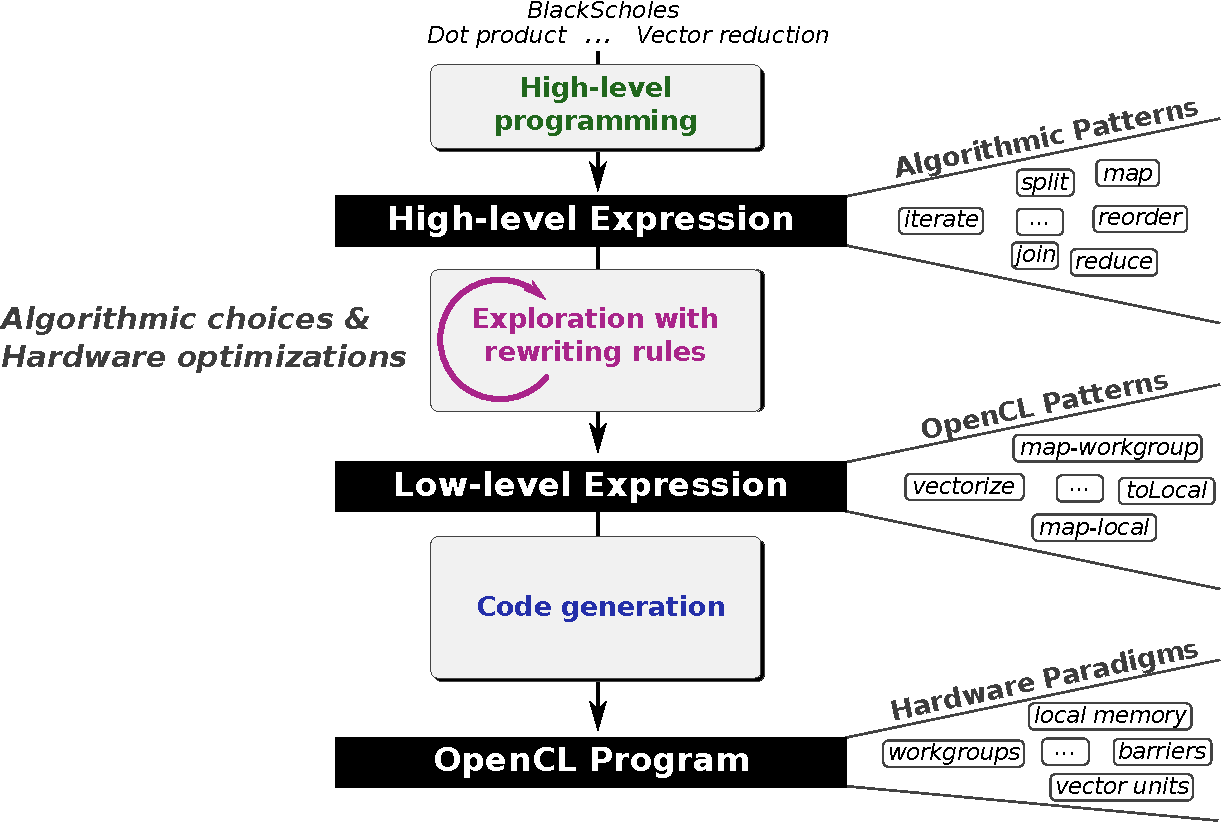
\includegraphics[width=\linewidth]{overviewPatternCodeGeneration}
\caption[Overview of our code generation approach.]{
Overview of our code generation approach.
The application developer expresses the problem with high-level algorithmic patterns.
These are systematically transformed into low-level \OpenCL patterns using a rule rewriting system.
\OpenCL code is generated by mapping the low-level patterns directly to the \OpenCL programming model representing hardware paradigms.
}
\label{fig:highlevel}
\end{figure}

\newpage
\section{Overview}
\label{section:code-generation:overview}

The overview of our pattern-based code generation approach is presented in \autoref{fig:highlevel}.
The programmer writes a \emph{high-level expression} composed of \emph{algorithmic patterns}.
Using a rewrite rule system, we transform (``\emph{lower}'') this high-level expression into a \emph{low-level expression} consisting of \emph{OpenCL patterns}.
At this rewrite stage, algorithmic and optimization choices in the high-level expression are explored.
The generated low-level expression is then fed into our code generator that emits an \emph{\OpenCL program} which is then compiled to machine code by the vendor-provided \OpenCL compiler.
A major advantage of our approach is that there is no analysis or optimizations performed in the code generator:
all optimization decisions are made earlier on in the rule rewrite system.
This results in a clear separation of concern between the high-level patterns used by the application developer and the low-level hardware paradigms that enable performance portability.


\newpage
\subsection{Introductory Example}

\begin{figure}[t]
\centering

\begin{subfigure}[b]{.85\linewidth}
\begin{lstlisting}[mathescape,numbers=left]
mul3 x     = x * 3    // user-defined function
vectorScal = map mul3          // map pattern
\end{lstlisting}
\caption{\textbf{High-level expression} written by the programmer.}
\label{fig:codeex:map}
\end{subfigure}

\begin{minipage}{0.1\linewidth}
\vspace{0pt}
\centering

\begin{tikzpicture}[ultra thick]
 \draw [black,   -latex      ] (0,0.5) -- (0,0) node [] {};
\end{tikzpicture}
\end{minipage}
\begin{minipage}{0.25\linewidth}
\vspace{-5pt}
\centering
\textbf{rewrite rules}
\end{minipage}
\begin{minipage}{0.1\linewidth}
\vspace{0pt}
\centering

\begin{tikzpicture}[ultra thick]
 \draw [black,   -latex      ] (0,0.5) -- (0,0) node [] {};
\end{tikzpicture}
\end{minipage}

\begin{subfigure}[b]{\linewidth}
\centering
\begin{minipage}{.85\linewidth}%{0.85\textwidth}
\begin{lstlisting}[mathescape,numbers=left]
mul3 x     = x * 3
vectorScal = join $\circ$ map-workgroup ($\label{fig:codeex:impl:map-wg}$
                    asScalar $\circ$ map-local ($\label{fig:codeex:impl:map-wg:start}$
                      vect 4 mul3$\label{fig:codeex:impl:vec}$
                    ) $\circ$ asVector 4$\label{fig:codeex:impl:map-wg:stop}$$\label{fig:codeex:impl:asVec}$
                 ) $\circ$ split 1024
\end{lstlisting}
\end{minipage}
\caption{\textbf{Low-level expression} derived using rewrite rules.}
\label{fig:codeex:impl}
\end{subfigure}

\begin{minipage}{0.1\linewidth}
\vspace{0pt}
\centering

\begin{tikzpicture}[ultra thick]
 \draw [black,   -latex      ] (0,0.5) -- (0,0) node [] {};
\end{tikzpicture}
\end{minipage}
\begin{minipage}{0.26\linewidth}
\vspace{-5pt}
\centering
\textbf{code generator}
\end{minipage}
\begin{minipage}{0.1\linewidth}
\vspace{0pt}
\centering

\begin{tikzpicture}[ultra thick]
 \draw [black,   -latex      ] (0,0.5) -- (0,0) node [] {};
\end{tikzpicture}
\end{minipage}

\begin{subfigure}[b]{\linewidth}
\centering
\begin{minipage}{.85\textwidth}
\begin{lstlisting}[mathescape,numbers=left]
float4 mul3(float4 x) { return x * 3; }$\label{fig:codeex:ocl:def}$

kernel vectorScal(global float* in,
                  global float* out, int len) {
 for (int i =get_group_id(0); i < len/1024;$\label{fig:codeex:ocl:loop1:start}$
          i+=get_num_groups(0)) {$\label{fig:codeex:ocl:loop1:end}$
  global float* grp_in  = in+(i*1024);
  global float* grp_out = out+(i*1024);
  for (int j =get_local_id(0); j < 1024/4;$\label{fig:codeex:ocl:loop2:start}$
           j+=get_local_size(0)) {$\label{fig:codeex:ocl:loop2:end}$
    global float4* in_vec4 =(float4*)grp_in+(j*4);
    global float4* out_vec4=(float4*)grp_out+(j*4);
    *out_vec4 = mul3(*in_vec4);$\label{fig:codeex:ocl:call}$
} } }  
\end{lstlisting}
\end{minipage}
\caption{\textbf{OpenCL program} produced by our code generator.}
\label{fig:codeex:ocl}
\end{subfigure}
\caption{
Pseudo-code representing vector scaling.
The user maps the \code{mul3} function over the input array~(\subref{fig:codeex:map}).
This high-level expression is transformed into a low-level expression~(\subref{fig:codeex:impl}) using rewrite rules.
Finally, our code generator turns the low-level expression into an \OpenCL program~(\subref{fig:codeex:ocl}).
}
  \label{fig:codeex}
\end{figure}

We illustrate the advantages of our approach using a simple vector scaling example shown in \autoref{fig:codeex}.
The user expresses the computation by writing a high-level expression using the algorithmic \pat{map} pattern as shown in \autoref{fig:codeex:map}.
This coding style is similar to functional and dataflow programming as well as the \SkelCL programming model introduced in \autoref{chapter:skelcl}.
As common in functional programming, the $\circ$ operator represents sequential function composition, \ie, $(f \circ g)\ x = f(g\ x)$.

Our technique first rewrites the high-level expression into a representation closer to the \OpenCL programming model.
This is achieved by applying rewrite rules which are presented later in \autoref{section:rules}.
\autoref{fig:codeex:impl} shows one possible derivation of the original high-level expression.
In the derived low-level expression, starting from the last line, the input is split into chunks of 1024 elements.
Each chunk is then mapped onto an \OpenCL work-group with the \pat{map-workgroup} low-level pattern (line~\ref{fig:codeex:impl:map-wg}).
Within a work-group (lines~\ref{fig:codeex:impl:map-wg:start}--\ref{fig:codeex:impl:map-wg:stop}), we vectorize the elements (line~\ref{fig:codeex:impl:asVec}), each mapped to a local work-item inside a work-group via the \pat{map-local} pattern (line~\ref{fig:codeex:impl:map-wg:start}).
\todo{sg: warum vectorize?}
Each local work-item now processes 4 elements, enclosed in a vector type.
Finally, the \pat{vect-4} pattern (line~\ref{fig:codeex:impl:vec}) vectorizes the user-defined function \code{mul3}.
The exact meaning of our patterns will be given later in \autoref{section:patterns}.

The last step consists of traversing the low-level expression and generating \OpenCL code for each low-level pattern encountered (\autoref{fig:codeex:ocl}).
The two map patterns generate the for-loops (line~\ref{fig:codeex:ocl:loop1:start}--\ref{fig:codeex:ocl:loop1:end} and~\ref{fig:codeex:ocl:loop2:start}--\ref{fig:codeex:ocl:loop2:end}) that iterate over the input array assigning work to the work-groups and local work-item.
The information of how many chunks each work-group and work-items processes comes from the corresponding \pat{split}.
\todo{sg: Warum 1024?}
In line~\ref{fig:codeex:ocl:call} the vectorized version of the user-defined \code{mul3} function (defined in line~\ref{fig:codeex:ocl:def}) is finally applied to the input array.

To summarize, our approach consists in generating \OpenCL code starting from a high-level program representation of a program.
This is achieved by systematically lowering the high-level expression into a low-level form suitable for code generation.
The next two sections present our high-level and low-level patterns, the code generation mechanism, and the rewrite rules.



\section{Patterns: Design and Implementation}
\label{section:patterns}

In this section, we will introduce the \emph{patterns} which form the expressions used for code generation.
As we saw in the previous section there exist two type of patterns: high-level algorithmic patterns and low-level \OpenCL patterns.
Some of the high-level algorithmic patterns directly correspond to algorithmic skeletons we have introduced in \autoref{chapter:skelcl}.
As we will also introduce patterns which we have not seen so far and which do not oblige to the common definition of algorithmic skeletons, we will use the more generic term \emph{pattern} throughout this and the next chapter.

The key idea of our approach is to expose algorithmic choices and hardware-specific program optimizations as patterns that are systematically derived using a rule rewriting system (discussed later in \autoref{section:rules}).
The high-level algorithmic patterns represent structured parallelism.
They can either be used by the programmer directly as a stand-alone language (or embedded domain specific language) or used as an intermediate representation targeted by the compiler of another language.
\todo{sg: embedded worin?}
Once a program is represented with our high-level patterns, we automatically transform the program into low-level patterns.
The low-level patterns represent hardware-specific concepts expressed by a programming model such as \OpenCL, which is the target chosen for this thesis.
Following the same approach, a different set of low-level patterns could be designed to target other low-level programming models such as Pthreads or MPI.


\subsection{High-level Algorithmic Patterns}

We define our patterns as functions.
To simplify our implementation, we encode all types as arrays with primitives represented by arrays of length 1.
The only exceptions are the user-defined functions, such as the \code{mul3} function in \autoref{fig:codeex:map} that operates on a primitive type.

\autoref{tab:hlskel} presents our high-level patterns used to define programs at the algorithmic level.
Most of the patterns are well known in functional programming, like \map and \reduce.
The \zip, \splitN and \join patterns transform the shape of the data.
For arrays we store the number of dimensions and size of each dimension in the type system, as we will see.
\todo{sg: we store ... in the type system. Wird das so gesagt?}
The \iterateN pattern iteratively applies a function multiple times.
Finally, the \reorder pattern lets our system know that it is safe to reorder the elements of an array arbitrarily, which enables additional optimizations -- as we will see later in \autoref{chapter:codeGeneration-evaluation}.

In the following, we discuss each high-level algorithmic pattern in more detail including their formal definitions.
As in \autoref{chapter:skelcl} we use the Bird-Meertens formalism~\cite{} as our syntax for the patterns.
\todo{add citation}

In this chapter we are especially interested in how patterns can be composed and nested.
As \emph{types} formally specify which compositions and nesting of patterns are legal, we will precisely define the type of each pattern.
% For expressing types we base our syntax on the syntax established by J. Roger Hindley, Robin Miler, and Luis Damas as part of the Hindley---Milner type system~\cite{}.
We write $e : \sigma$ to denote that expression $e$ has type $\sigma$.
% To make typing judgments we write $e_0 : \sigma_0,\ \ldots,\ e_n : \sigma_n\ \vdash e : \sigma$ to denote that under the assumptions that $e_0,\ \ldots,\ e_n$ have types $\sigma_0,\ \ldots,\ \sigma_n$ the expression $e$ has type $\sigma$.
For a function mapping values of type $\alpha$ to values of type $\beta$ we write its type as $(\alpha \rightarrow \beta)$.
Tuple types are written as $\langle\alpha, \beta\rangle$.
Finally, arrays have their length denoted as part of their type:
for an array with elements of type $\alpha$ and length $n$, we write $[\alpha]_n$.

\begin{table}[t]
\centering
\begin{tabular}{p{.1\textwidth}p{.85\textwidth}}
\toprule
\tabhead{Pattern} & \tabhead{Description}\\
\midrule
 \map
     & Apply a given function to every element of an input array.\\ 
 \reduce
     & Perform a reduction of an input array using a user-defined binary function and an initial value.\\
 \zip
     & Build an array of pairs by pairwise combining two arrays.\\
 \splitN
     & Produce a multi-dimensional array by splitting an array in chunks of a given size.\\
 \join
     & Join the two outer most dimensions of an multi-dimensional array.\\
 \iterateN
     & Iterate a given function over an input array a fixed number of times.\\
 \reorder
     & Reorder the element of the input array.\\
\bottomrule
\end{tabular}
\caption{High-level algorithmic patterns used by the programmer.}
\label{tab:hlskel}
\end{table}


\paragraph{Map}
The \map pattern is well known in functional programming and applies a given unary function $f$ to all elements of an input array.
In \autoref{chapter:skelcl}, we defined the \map pattern as an algorithmic skeleton (see \autoref{definition:map}).
The same definition holds here.
We repeat it here for completeness and we add the type information:
\begin{definition}
  \label{definition:pattern:map}
  Let $\vec{x}$ be an array of size $n$ with elements $x_i$ where $0 < i \leq n$.
  Let $f$ be a unary customizing function defined on elements.
  The \map pattern is then defined as follows:
  \begin{equation*}
    \map\ f\ [x_1, x_2, \dots, x_n] \eqdef [f\ x_1, f\ x_2, \dots, f\ x_n]
  \end{equation*}
  The types of $f$, $\vec{x}$, and \map are as follows:
  \begin{align*}
    f &: (\alpha \rightarrow \beta),\\
    \vec{x} &: [\alpha]_n,\\
    \map\ f\ \vec{x} &: [\beta]_n
  \end{align*}
\end{definition}

\noindent
In \autoref{chapter:skelcl} we also defined the \map skeleton for operating on matrices (see \autoref{definition:map:matrix}).
In this chapter we represent matrices as nested arrays, therefore, performing an operation on each element of a matrix can be represented by nesting two \map patterns:
\begin{align*}
  mapMatrix\ \ f\ \ X &= \map\ (\map\ f)\ X
\end{align*}
Let us assume that $X$ represents an $n\times m$ matrix with elements of type $\alpha$, then its type is $\big[[\alpha]_m\big]_n$.
The outer \map applies its customizing function to every row of matrix $X$.
The customizing function is defined by \emph{currying}~\cite{} \map and $f$, thus, producing a function which applies $f$ to every element of its argument array.
\todo{add citation for currying}
Therefore, $f$ will be applied to every element of matrix $X$.

\paragraph{Reduce}
The \reduce pattern (\aka, fold or accumulate) uses a given binary function $f$ to combine all elements of the input array.
We require the function $f$ to be associative and commutative which allows for an efficient parallel implementation.
By requiring commutativity, our system can also generate vectorized implementations of the reduction and utilize the efficient coalesced memory access pattern, as we saw in \autoref{section:reduce:case-study}.
In \autoref{chapter:skelcl} we defined \reduce as an algorithmic skeleton (see \autoref{definition:reduce}).
The same definition holds here.
We repeat it here for completeness and we add the type information:
\begin{definition}
  \label{definition:pattern:reduce}
  Let $\vec{x}$ be an array of size $n$ with elements $x_i$ where $0 < i \leq n$.
  Let $\oplus$ be an associative and commutative binary customizing operator with the identity element \id.
  The \reduce pattern is then defined as follows:
  \begin{equation*}
    \reduce\ \oplus\ \id\ [x_1, x_2, \dots, x_n]
      \eqdef x_1 \oplus x_2 \oplus \dots \oplus x_n
  \end{equation*}
  The types of $\oplus$, $\id$, $\vec{x}$, and \reduce are as follows:
  \begin{align*}
    \oplus &: ((\alpha, \alpha) \rightarrow \alpha),\\
    \id &: \alpha,\\
    \vec{x} &: [\alpha]_n,\\
    \reduce\ \oplus\ \id\ \vec{x} &: [\alpha]_1
  \end{align*}
\end{definition}
\todo{sg: vielleicht sagen, dass wir id manchmal omitten reduce (+) [ ]?}


\paragraph{Zip}
The \zip pattern and the following \splitN/\join patterns transform the shape of the data. %which we store in the type system, \ie, number of dimensions and size of each dimension.
The \zip pattern fuses two arrays into a single array of pairs.

\begin{definition}
  \label{definition:pattern:zip}
  Let $\vec{x}$ and $\vec{y}$ be arrays of size $n$ with elements $x_i$ and $y_i$ where $0 < i \leq n$.
  The \zip pattern is then defined as follows:
  \begin{equation*}
    \zip\ [x_1, x_2, \dots, x_n]\ [y_1, y_2, \dots, y_n]\\
      \eqdef [\langle x_1, y_1\rangle, \langle x_2, y_2\rangle, \dots, \langle x_n, y_n\rangle]
  \end{equation*}
  The types of $\vec{x}$, $\vec{y}$, and \zip are as follows:
  \begin{align*}
    \vec{x} &: [\alpha]_n,\\
    \vec{y} &: [\beta]_n,\\
    \zip\ \vec{x}\ \vec{y} &: [\langle\alpha, \beta\rangle]_n
  \end{align*}
\end{definition}

\noindent
This definition significantly differs from the definition of the \zip skeleton in \autoref{chapter:skelcl}:
While in \autoref{definition:zip}, \zip applies a given function to a pair of elements, there is no function to be applied in \autoref{definition:pattern:zip} of the \zip pattern.
The behavior of the \zip skeleton can be achieved by composing the \zip pattern with the \map pattern:
\begin{align*}
  zipWith\ f\ \vec{x}\ \vec{y} &= \map\ f\ (\zip\ \vec{x}\ \vec{y})
\end{align*}


\paragraph{Split and Join}
The \splitN pattern, which is most often combined with a \join, partitions an array into chunks of specific size, resulting in an extra dimension in the output array.

We start with the definition of the \splitN pattern.
\begin{definition}
  \label{definition:pattern:split}
  Let $n$ be an integer value.
  Let $\vec{x}$ be an array of size $m$ with elements $x_i$ where $0 < i \leq m$.
  Let us assume that $m$ is evenly divisible by $n$.
  The \splitN pattern is then defined as follows:
  \begin{align*}
    &\splitN\ n\ [x_1, x_2, \dots, x_m] \eqdef\\
    &\qquad\big[[x_1, \ldots, x_n], [x_{n+1}, \ldots, x_{2n}], \ldots, [x_{m-n+1}, \ldots, x_m]\big]
  \end{align*}
  The types of $n$, $\vec{x}$, and \splitN are as follows:
  \begin{align*}
    n &: int,\\
    \vec{x} &: [\alpha]_n,\\
    \splitN\ n\ \vec{x} &: \big[[\alpha]_n\big]_{\frac{m}{n}}
  \end{align*}
\end{definition}

\bigskip
%The formal type of the \splitN pattern is:
%\begin{align}
%  n : int,\ xs : [\alpha]_m\ \vdash\ split\ n\ xs : \big[[\alpha]_n\big]_{{}^m/_n}
%\end{align}

\noindent
The corresponding \join pattern does the opposite:
it reassembles an array of arrays by merging dimensions.
\begin{definition}
  \label{definition:pattern:join}
  Let $\vec{x}$ be an array of size $\frac{m}{n}$ whose elements are arrays of size $n$.
  We denote the elements of the $i$th inner array as $x_{((i-1)\times n) + j}$ where $0 < i \leq \frac{m}{n}$ and $0 < j \leq n$.
  The \join pattern is then defined as follows:
  \begin{align*}
    &\join\ \big[[x_1, \ldots, x_n], [x_{n+1}, \ldots, x_{2n}], \ldots, [x_{m-n+1}, \ldots, x_m]\big] \eqdef\\
    &\qquad[x_1, x_2, \dots, x_m]
  \end{align*}
  The types of $n$, $m$, $\vec{x}$, and \join are as follows:
  \begin{align*}
    n &: int, m : int,\\
    \vec{x} &: \big[[\alpha]_n\big]_{\frac{m}{n}},\\
    \join\ \vec{x} &: [\alpha]_n
  \end{align*}
\end{definition}

\noindent
From these definitions it follows, that the composition of $\splitN\ n$ and \join: $\join \circ \splitN\ n$ for any value $n$ yields the same type and also does not change any element in the array, \ie, it is equivalent to the identify function \emph{id}.

These two patterns used together are similar to the split-join concept from data-flow languages such as StreamIt~\cite{ThiesKaAm2002}.


\paragraph{Iterate}
The \iterateN pattern corresponds to the mathematical definition of iteratively applying a function, which is defined as: {$f^0 = id$} and {$f^{n+1} = f^n \circ f$}.

\begin{definition}
  \label{definition:pattern:iterate}
  Let $n$ be an integer value with $n \geq 0$.
  Let $f$ be a unary function on arrays.
  Let $\vec{x}$ be an array of arbitrary size.
  We define the \iterateN pattern recursively:
  \begin{align*}
    \iterateN\ n\ f\ \vec{x} &\eqdef \iterateN\ (n-1)\ f\ (f\ \vec{x}),\\
    \iterateN\ 0\ f\ \vec{x} &\eqdef \vec{x}
  \end{align*}
  The types of $n$, $f$, $\vec{x}$, and \iterateN are as follows:
  \begin{align*}
    n &: int,\\
    f &: ([\alpha]_k \rightarrow [\alpha]_{F(k)}), 
      \begin{aligned}[t]
        & \forall k \text{ and where } \\
        &F : (int\rightarrow int) \text{ describes the change}\\
        &\text{of array length when applying } f,
      \end{aligned}\\
    \vec{x} &: [\alpha]_m,\\
    \iterateN\ n\ f\ \vec{x} &: [\alpha]_{F^n(m)}
  \end{align*}
\end{definition}


% In terms of implementation, our code generator emits a for-loop to perform the iteration, and two pointers for input and output.
% After each iteration, we swap the pointers, so that the output of the last iteration becomes the input for the next one.
% We automatically allocated and calculate memory requirements based on the information from the input and output type.
\noindent
\todo{say more}
The type property of the \iterateN pattern is interesting as its result type depends on the effect $f$ has on the size of its argument.

%\begin{align}
%  n : int,\ F : (int \rightarrow int),\ f : (\forall k\ .\ [\alpha]_k \rightarrow [\alpha]_{F(k)}),\ xs : [\alpha]_m\ %
%  \vdash iterate\ n\ f\ xs : [\alpha]_{F^{n}(m)}
%\end{align}

\paragraph{Reorder}
The \reorder pattern is used to specify that the ordering of the elements of an array does not matter.

\begin{definition}
  \label{definition:pattern:reorder}
  Let $\vec{x}$ be an array of size $n$ with elements $x_i$ where $0 < i \leq n$.
  Let $\sigma$ be an arbitrary permutation of $[1,\ldots, n]$.
  The \reorder pattern is then defined as follows:
  \begin{align*}
    \reorder\ [x_1, \ldots, x_n] &\eqdef [x_{\sigma(1)}, \ldots, x_{\sigma(n)}]
  \end{align*}
  The types of $\vec{x}$ and \reorder are as follows:
  \begin{align*}
    \vec{x} &: [\alpha]_n,\\
    \reorder\ \vec{x} &: [\alpha]_n
  \end{align*}
\end{definition}

\noindent
This definition allows the implementation to pick any permutation to reorder the elements of an array arbitrarily which may enable optimizations, as we will see later.





\subsection{Low-level, \OpenCL-specific Patterns}

% Programming manycore CPU and GPU devices is difficult due to the need for managing parallelism, the memory hierarchy and other hardware specific features.
In order to achieve the highest performance, programmers often use a set of intuitive ``rules of thumb'' to optimize their applications.
We extensively discussed one application example in \autoref{section:reduce:case-study}.
Each hardware vendor provides own optimization guides~\cite{CUDAProgrammingGuide,AMDProgrammingGuide,IntelGPUProgrammingGuide,IntelXeonProgrammingGuide} that extensively cover vendor's hardware particularities and optimizations.
The main idea behind our approach is to identify common optimization patterns and express them systematically rather than intuitively, with the help of low-level patterns coupled with a rewrite-rule system.

\autoref{tab:llskel} gives an overview of the \OpenCL-specific patterns we have identified.

\begin{table}[t]
\centering
\begin{tabular}{p{.25\textwidth}p{.7\textwidth}}
\toprule
\tabhead{Pattern} & \tabhead{Description}\\
\midrule
 \mapWorkgroup
     & Each \OpenCL \textbf{work-group} applies the given function to an element of the input array.\\
 \mapLocal
     & Each \textbf{local work-item} of a work-group applies the given function to an element of the input array.\\ 
 \mapGlobal
     & Each \textbf{global work-item} applies the given function to an element of the input array.\\ 
 \mapWarp
     & Each \textbf{warp} applies the given function to an element of the input array.\newline Only available for Nvidia \GPUs.\\
 \mapLane
     & Each \textbf{work item inside a warp} applies the given function to an element of the input array.\newline Only available for Nvidia \GPUs.\\
 \mapSeq
      & Apply the given function to every element of the input array \textbf{sequentially}.\\
 \reduceSeq
      & Perform the reduction using the given binary reduction function and initial value on the input array \textbf{sequentially}.\\  
 \reorderStride
      & Access input array with a given stride to maintain \textbf{memory coalescing}.\\
 \toLocal
      & Store the results of a given function to \textbf{local memory}.\\
 \toGlobal
      & Store the results of a given function to \textbf{global memory}.\\
 \asVector
      & Turns the elements of an array into \textbf{vector type} of a given width.\\
 \asScalar
      & Turns the elements of an array into \textbf{scalar type}.\\
 \vect
      & \textbf{Vectorize} a given function by a given width.\\
\bottomrule
\end{tabular}
\caption{Low-level \OpenCL patterns used for code generation.}
\label{tab:llskel}
\end{table}

\paragraph{Parallel Maps}
The different \OpenCL \map patterns represent possible ways of mapping computations to the hardware and exploit thread-level parallelism in \OpenCL.
The execution semantics and types of all these low-level \OpenCL \map patterns are the same as of the high-level \map pattern shown in \autoref{definition:pattern:map}.
In fact, these patterns can be viewed as \emph{instantiations} of the high-level \map pattern \emph{interface}, as they provide different possibilities to implement the \map pattern.
\todo{sg: was ist ein pattern interface?}

\todo{sg: hier waere ein Bild gut, das diese maps zusammen mit der OpenCL Thread-Hierarchie zeigt}
The \mapWorkgroup pattern assigns work to an \OpenCL work-group, \ie, following \autoref{definition:pattern:map} each \OpenCL work-group executes the given function on a different part of the input vector.

The \mapLocal pattern assigns work to a local work-item inside a work-group.
This pattern should be used in the context of a work-group and is, therefore, only valid when nested inside a \mapWorkgroup pattern, \eg, $\mapWorkgroup\ (\mapLocal\ f)$.

The \mapGlobal pattern can be used to assign work to work-items outside of a work-group.
This allows us to map computations in different ways to the thread hierarchy of \OpenCL.

%The code generation for all these map patterns is similar; we describe it using \pat{map-workgroup} as an example.
%A loop is generated, where the iteration variable is determined by the \emph{workgroup-id} function provided by \OpenCL.
%Inside of the loop, a pointer is generated to partition the input array, so that every work-group calls \pat{map-workgroup}'s customizing function on a different chunk of data.
%An output pointer is generated similarly.
%We continue with the body of the loop by generating the code for the customizing function recursively.
%Finally, an appropriate synchronization mechanism for the given map pattern is added.
%For instance after a \pat{map-local} we add a barrier synchronization to synchronize the threads inside of the work-group.

\paragraph{Sequential Map and Reduce}
The \mapSeq and \reduceSeq patterns perform a sequential map and reduction, respectively, within a single work-item.
% In both cases the generated code consists of a loop iterating over the array and calling the customizing function.
% For the reduction an accumulation variable is initialized with the given initial value and used to accumulate the results produced by the successive calls to to the customizing function.

For the \mapSeq pattern, the semantics and type are the same as for the high-level \map pattern shown in \autoref{definition:pattern:map}.
This is not the case for the \reduceSeq and \reduce patterns, where their types differ.
For the high-level \reduce pattern, we require the customizing binary function to be associative and commutative in order to allow for an efficient parallel implementation.
As the \reduceSeq pattern performs a sequential reduction, we can relax these requirements, therefore, we define \reduceSeq separately.
\begin{definition}
  \label{definition:pattern:reduceSeq}
  Let $\vec{x}$ be an array of size $n$ with elements $x_i$ where $0 < i \leq n$.
  Let $\oplus$ be a binary customizing operator with the identity element \id.
  The \reduceSeq pattern is then defined as follows:
  \begin{equation*}
    \reduceSeq\ \oplus\ \id\ [x_1, x_2, \dots, x_n]
      \eqdef (\dots((id \oplus x_1) \oplus x_2) \ldots \oplus x_n)
  \end{equation*}
  The types of $\oplus$, $\id$, $\vec{x}$, and \reduce are as follows:
  \begin{align*}
    \oplus &: ((\alpha, \beta) \rightarrow \alpha),\\
    \id &: \alpha,\\
    \vec{x} &: [\beta]_n,\\
    \reduceSeq\ \oplus\ \id\ \vec{x} &: [\alpha]_1
  \end{align*}
\end{definition}

\todo{sg: Table 5.2 hier platzieren}


\paragraph{Reorder-stride}
The \reorderStride pattern enforces a special reordering of an array.
\todo{sg: definition??}
In our implementation no code is produces, but rather the reordering determines how the data is read from the array.
The produced strided-access pattern ensures that after splitting the workload, consecutive work-items access consecutive memory elements.
This corresponds to the \emph{coalesce memory accesses}, which are beneficial on modern \GPUs as discussed in \autoref{chapter:background}.

\begin{definition}
  \label{definition:pattern:reorderStride}
  Let $s$ be an integer value.
  Let $\vec{x}$ be an array of size $m$ with elements $x_i$, where $0 < i \leq m$.
  Let us assume that $m$ is evenly divisible by $s$ and that $m = s\times n$ for some integer value $n$.
  The \reorderStride pattern is then defined as follows:
  \begin{align*}
    \reorderStride\ s\ [x_1, x_2, \dots, x_m] &\eqdef [y_1, y_2, \dots, y_m], \text{ where}\\
    y_i &\eqdef x_{i / n + s \times (i \bmod{n})}
  \end{align*}
  The types of $s$, $\vec{x}$, and \reorderStride are as follows:
  \begin{align*}
    s &: int,\\
    \vec{x} &: [\alpha]_m,\\
    \reorderStride\ s\ \vec{x} &: [\alpha]_m
  \end{align*}
\end{definition}

%\noindent
\todo{Maybe a figure visualizing the reordering ...}

%Our implementation does not produce code directly, but generates instead an index function, which is used when accessing the array the next time.
%Therefore, any following read implicitly reorders the array.
%Our design is general enough to supports user-defined index functions as well, which we will add in the future.
%The type of \pat{reorder-stride} corresponds to the type of the high-level \pat{reorder} pattern.

\paragraph{{\footnotesize to}Local and {\footnotesize to}Global}
The \toLocal and \toGlobal patterns are used to specify where the result of a given function $f$ should be stored.
As explained in more detail in \autoref{chapter:background}, \OpenCL defines two distinct address spaces: global and local.
Global memory is the commonly used large but slow memory.
On \GPUs, the comparatively small local memory has a high bandwidth with low latency and is used to store frequently accessed data.
With these two patterns, we can in effect exploit the memory hierarchy defined in \OpenCL.

First, we define \toLocal:
\begin{definition}
  \label{definition:pattern:toLocal}
  Let $f$ be a function.
  The \toLocal pattern is then defined as follows:
  \begin{align*}
    \toLocal\ f &\eqdef f',
    \begin{aligned}[t]
      &\text{ where $f'\ x \eqdef f\ x$, $\forall x$, and  $f'$ is guaranteed to store}\\
      &\text{its result in local memory.}
    \end{aligned}
  \end{align*}
  The types of $f$, and \toLocal are as follows:
  \begin{align*}
    f &: (\alpha \rightarrow \beta)\\
    \toLocal\ f &: (\alpha \rightarrow \beta)
  \end{align*}
\end{definition}

\noindent
The definition of \toGlobal is correspondent:
\begin{definition}
  \label{definition:pattern:toGlobal}
  Let $f$ be a function.
  The \toGlobal pattern is then defined as follows:
  \begin{align*}
    \toGlobal\ f &\eqdef f',
    \begin{aligned}[t]
      &\text{ where $f'\ x \eqdef f\ x$, $\forall x$ and $f'$ is guaranteed to store}\\
      &\text{ its result in global memory.}
    \end{aligned}
  \end{align*}
  The types of $f$, and \toGlobal are as follows:
  \begin{align*}
    f &: (\alpha \rightarrow \beta)\\
    \toGlobal\ f &: (\alpha \rightarrow \beta)
  \end{align*}
\end{definition}

% These patterns act similarly to a typecast and are in fact implemented as such so that no code is emitted directly.

%In our design, every function reads its input and writes its output using pointers provided by the callee function.
%As a result, we can simply force a store to local memory by wrapping any function with our \pat{toLocal} pattern.
%In the code generator, this will simply change the output pointer of function $f$ to an area in local memory.

%The types of \pat{toLocal} and \pat{toGlobal} are identical and as follows:
%\begin{align}
%  f : (\alpha \rightarrow \beta)\ &\vdash\ toLocal\ f : (\alpha \rightarrow \beta)
%  \label{eq:type:toLocal}
%  \\
%  f : (\alpha \rightarrow \beta)\ &\vdash\ toGlobal\ f : (\alpha \rightarrow \beta)
%  \label{eq:type:toGlobal}
%\end{align}


\paragraph{{\footnotesize as}Vector, {\footnotesize as}Scalar, and Vectorize}
The \OpenCL programming model supports vector data types such as \code{float4} where any operations on this type will be executed in the hardware vector units.
In the absence of vector units in the hardware, the \OpenCL compiler scalarizes the code automatically.
\todo{sg: scalarizes, wird das so gesagt?}

The \asVector and \asScalar patterns change the data type into vector elements and scalar elements, correspondingly.
For instance, an array of \code{float} is transformed into an array of \code{float4} as seen in the motivation example (\autoref{fig:codeex}).
The \vect pattern vectorizes the given function by simply converting all the operations that apply to vector types into vectorized operations. 
%Our current implementation can only vectorize functions containing simple arithmetic operations such as $+$ or $-$.
In case of more complex functions, we rely on external tools~\cite{KarrenbergHa2011} for vectorizing the operations.
%These tools are not required to performing further analysis to find opportunities for vectorization.
%The rewrite rules presented in \autoref{section:rules} ensure that vectorization is only applied to patterns where vectorization is a legal optimization.

We start by defining the \asVector pattern.
\begin{definition}
  \label{definition:pattern:asVector}
  Let $n$ be an integer value.
  Let $\vec{x}$ be an array of size $m$ with elements $x_i$ where $0 < i \leq m$.
  Let us assume, that $m$ is evenly divisible by $n$.
  The \asVector pattern is then defined as follows:
  \begin{align*}
    &\asVector\ n\ [x_1, x_2, \dots, x_m] \eqdef \\
    &\qquad\big[\{x_1, \ldots, x_n\}, \{x_{n+1}, \ldots, x_{2n}\}, \ldots, \{x_{m-n+1}, \ldots, x_m\}\big],
  \end{align*}
  where $\{x_1,\ldots,x_n\}$ denotes a vector of width $n$.\\
  The types of $n$, $\vec{x}$, and \asVector are as follows:
  \begin{align*}
    n &: int\\
    \vec{x} &: [\alpha]_m,\\
    \asVector\ n\ \vec{x} &: [\alpha_n]_{\frac{m}{n}}
  \end{align*}
  Here $\alpha$ is required to be a basic scalar type, \eg, \code{int} or \code{float}, and $\alpha_n$ denotes the vectorized version of that type with a vector width of $n$.
\end{definition}

\noindent
The corresponding \asScalar pattern is defined as follows.
\begin{definition}
  \label{definition:pattern:asScalar}
  Let $\vec{x}$ be an array of size $\frac{m}{n}$ whose elements are vectors of width $n$.
  We denote the individual vector elements of the $i$th element of $\vec{x}$ as $x_{((i-1)\times n)+j}$ where $0 < i \leq \frac{m}{n}$ and $0 < j \leq n$.
  The \asScalar pattern is then defined as follows:
  \begin{align*}
    &\asScalar\ \big[\{x_1, \ldots, x_n\}, \{x_{n+1}, \ldots, x_{2n}\}, \ldots, \{x_{m-n+1}, \ldots, x_m\}\big] \eqdef\\
    &\qquad [x_1, x_2, \dots, x_m],
  \end{align*}
  where $\{x_1,\ldots,x_n\}$ denotes a vector of width $n$.\\
  The types of $n$, $\vec{x}$, and \asVector are as follows:
  \begin{align*}
    n &: int\\
    \vec{x} &: [\alpha_n]_{\frac{m}{n}},\\
    \asVector\ n\ \vec{x} &: [\alpha]_m
  \end{align*}
  Here $\alpha$ is required to be a basic scalar type, \eg, \code{int} or \code{float}, and $\alpha_n$ denotes the vectorized version of that type with a vector width of $n$.
\end{definition}

\noindent
Finally, we define th \vect pattern.
\begin{definition}
  \label{definition:pattern:vect}
  Let $n$ be an integer value.
  Let $f$ be a function.
  The \vect pattern is then defined as follows:
  \begin{align*}
    \vect\ n\ f &\eqdef f'_n, \begin{aligned}[t]
      \text{ where $f'_n$ is a vectorized version of $f$}\\
      \text{ for a vector width of $n$. }
    \end{aligned}
  \end{align*}
  The types of $n$, $f$, and \vect are as follows:
  \begin{align*}
    n &: int,\\
    f &: (\alpha \rightarrow \beta),\\
    \vect\ n\ f &: (\alpha_n \rightarrow \beta_n)
  \end{align*}
  Here $\alpha$ and $\beta$ are required to be a basic scalar type, \eg, \code{int} or \code{float}, and $\alpha_n$ denotes the vectorized version of that type with a vector width of $n$.
\end{definition}

\subsection{Summary}
In this section we introduced two type of \emph{patterns}:
high-level algorithmic patterns and low-level, \OpenCL-specific patterns.
While all of these patterns can be used by the application programmer to describe the solution for a particular problem, we expect the programmer to focus on the algorithmic patterns which should be used to express a high-level algorithmic implementation of the problem solution.
We will see in the next section how such an implementation composed of our high-level algorithmic patterns can be systematically rewritten using \emph{rewrite rules}.
During this process the original implementation will be modified and \OpenCL-specific patterns will be used.




\section{Rewrite Rules}
\label{section:rules}

This section introduces our set of rewrite rules that transform high-level expressions written using our algorithmic patterns into semantically equivalent expressions.
One goal of our approach is to keep each rule as simple as possible and only express one fundamental concept at a time.
For instance the vectorization rule, as we will see, is the only rule expressing the vectorization concept.
This is different from most previous library or compiler approaches which provide or produce a special vectorized version of different algorithmic patterns such as map or reduce.
The advantage of our approach lies in the power of composition:
many rules can be applied successively to produce expressions that compose hardware concepts or optimizations and that are provably correct by construction.

Similarly to our patterns, we distinguish between algorithmic and \OpenCL-specific rules.
Algorithmic rules produce derivations that represent different algorithmic choices.
Our \OpenCL-specific rules map expressions to \OpenCL patterns.
Once the expression is lowered and consist only of \OpenCL patterns, it is possible to produce \OpenCL code for each single pattern straightforwardly with our code generator as described in the following section.

We write $a \rightarrow b$ for a rewrite rule which allows to replace the occurrence of term $a$ in an expression with term $b$.
Sometimes multiple rewrites are valid then we write $a \rightarrow b\ |\ c$ to indicate the choice to replace term $a$ either with term $b$ or term $c$.

For each rule we provide a proof of its correctness, \ie, that applying the rewrite rule does not change the semantic of the expression the rule is applied to.

%We discuss some proofs of the rules here to give an idea how the correctness of the rules can be formally proven.
%The proofs for all rules can be found in the appendix in \autoref{}.

%\paragraph{Syntax and Rule Derivation}
%Some rules can only be activated if certain conditions are true.
%We use the syntax $[pre:post]$ to represent the pre and post conditions of a rule.
%The pre condition $pre$ corresponds to the list of conditions that must be true for the rule to be applied.
%The post condition $post$ is set for any function bound to the pattern.
%The $\overline{\rule[-.3\baselineskip]{0pt}{1.5ex}\hspace{1.5ex}}$, $\wedge$, and $\vee$ corresponds to the logical \emph{not}, \emph{and}, and \emph{or} operators respectively.

%We use leftmost derivation when applying the rules, which means that the leftmost non-terminal is always derived first.

\newenvironment{rerule}[1]%
{\begin{equation}\begin{array}{#1}\ignorespaces}%
{\end{array}\end{equation}%
\ignorespacesafterend}

\newenvironment{rerule*}[1]%
{\begin{equation*}\begin{array}{#1}\ignorespaces}%
{\end{array}\end{equation*}%
\ignorespacesafterend}


\newcommand{\comment}[1] {%
\{\text{\small #1}\}%
}

\subsection{Algorithmic Rules}
\label{section:rules:algo}

Each algorithmic rule formulates a provably correct statement of the relationship of multiple algorithmic patterns.
Applying the rules allows to rewrite an expression and, by doing so, explore different implementations.
As the algorithmic rules are separated from the  \OpenCL rules, these rules can explore valid implementations regardless of their concrete implementation in a concrete low-level programming model like \OpenCL.

\paragraph{Identity}
The identity rule in \autoref{eq:algo:identity} specifies that it is always valid to compose any function $f$ with the identity function \emph{id}.
As we always operate on arrays, we technically compose $f$ with $\map\ id$.
%
\begin{rerule}{lclcl}
  f & \rightarrow & f \circ \map\ \textit{id} & | & \map\ \textit{id} \circ f
  \label{eq:algo:identity}
\end{rerule}
%
The \textit{id} function can act as a copy operation; this is, \eg, useful for expressing copies of an array to local memory when composed with the \toLocal \OpenCL pattern: $\toLocal\ (\map\ \textit{id})$.

\begin{proof}[Proof of \autoref{eq:algo:identity}; option 1]
  Let $xs = [x_1, \ldots, x_n]$.
  \begin{align*}
    (f \circ \map\ \textit{id})\ xs
      &= f\ (\map\ \textit{id}\ xs)\\
      &\begin{aligned}[t]
        & \comment{definition of \map}                                         && \comment{definition of \textit{id}}\\
        &= f\ ([\textit{id}\ x_1, \textit{id}\ x_2, \ldots, \textit{id}\ x_n]) &&= f\ xs
      \end{aligned}
  \end{align*}
\end{proof}
\begin{proof}[Proof of \autoref{eq:algo:identity}; option 2]
  Let $xs = [x_1, \ldots, x_n]$.
  \begin{align*}
    (\map\ \textit{id} \circ\ f)\ xs
      &= \map\ \textit{id}\ (f\ xs)\\
      & \comment{definition of \map}\\
      &= [\textit{id}\ (f\ xs)_1, \textit{id}\ (f\ xs)_2, \ldots, \textit{id}\ (f\ xs)_n]\\
      & \comment{definition of \textit{id}}\\
      &= f\ xs
  \end{align*}
\end{proof}


\paragraph{Iterate decomposition}
The rule in \autoref{eq:algo:iterate} expresses the fact that an iteration can be decomposed into several iterations.
%
\begin{rerule}{lcl}
  \iterateN\ 1\ f & \rightarrow & f\\
  \iterateN\ (m+n)\ f
    & \rightarrow &
      \iterateN\ m\ f
        \circ \iterateN\ n\ f
  \label{eq:algo:iterate}
\end{rerule}

\begin{proof}[Proof of \autoref{eq:algo:iterate}; option 1]
  \begin{align*}
      & \comment{definition of \iterateN} && \comment{definition of \iterateN}\\
    \iterateN\ 1\ f\ xs
      &= \iterateN\ (1-1)\ f\ (f\ xs) \hspace{-5em}&& = f\ xs
  \end{align*}
\end{proof}
\begin{proof}[Proof of \autoref{eq:algo:iterate}; option 2]
  Proof by induction over the natural number $n$.
  We start with the base case, let $n=0$:
  \begin{align*}
      & \comment{definition of \iterateN}\\
    \iterateN\ (m+0)\ f\ xs
      &= \iterateN\ m\ f\ (\iterateN\ 0\ f\ xs)\\
      & \comment{definition of \iterateN}\\
      &= (\iterateN\ m\ f \circ \iterateN\ 0\ f)\ xs
  \end{align*}
  We finish with the induction step $n-1 \rightarrow n$:
  \begin{align*}
      & \comment{definition of \iterateN}\\
    \iterateN\ (m+n)\ f\ xs
      &= \iterateN\ (m+n-1)\ f\ (f\ xs)\\
      & \comment{induction hypothesis}\\
      &= (\iterateN\ m\ f\ \circ \iterateN\ (n-1)\ f) (f\ xs)\\
      & \comment{definition of $\circ$}\\
      &= \iterateN\ m\ f\ (\iterateN\ (n-1)\ f\ (f\ xs))\\
      & \comment{definition of \iterateN}\\
      &= \iterateN\ m\ f\ (\iterateN\ n\ f\ xs)\\
      & \comment{definition of $\circ$}\\
      &= (\iterateN\ m\ f \circ \iterateN\ n\ f)\ xs
  \end{align*}
\end{proof}


\paragraph{Reorder commutativity}
The following \autoref{eq:algo:reorder} shows that if the data can be reordered arbitrarily, as indicated by the \reorder pattern, then, it does not matter if we apply a function $f$ to each element before or after the reordering.
%
\begin{rerule}{lcl}
  \map\ f \circ \reorder
    & \rightarrow & \reorder \circ \map\ f\\
  \reorder \circ \map\ f
    & \rightarrow & \map\ f \circ \reorder
  \label{eq:algo:reorder}
\end{rerule}

\begin{proof}[Proof of \autoref{eq:algo:reorder}]
  We start with the expression $\map\ f \circ \reorder$.
  Let $xs = [x_1, \ldots, x_n]$.
  \begin{align*}
    (\map\ f \circ \reorder)\ xs
      &= \map\ f\ (\reorder\ xs)\\
      & \comment{definition of \reorder}\\
      &= \map\ f\ [x_{\sigma(1)}, \ldots, x_{\sigma(n)}]\\
      & \comment{definition of \map}\\
      &= [f\ x_{\sigma(1)}, \ldots, f\ x_{\sigma(n)}]
  \end{align*}
  Now we investigate the expression $\reorder \circ \map\ f$:
  \begin{align*}
    (\reorder \circ \map\ f)\ xs
      &= \reorder\ (\map\ f\ xs)\\
      & \comment{definition of \map}\\
      &= \reorder\ [f\ x_1, \ldots, f\ x_n]\\
      &= \reorder\ [y_1, \ldots, y_n]\qquad \text{with } y_i = f\ x_i\\
      & \comment{definition of \reorder}\\
      &= [y_{\sigma(1)}, \dots, y_{\sigma(n)}]\\
      & \comment{definition of $y_i$}\\
      &= [f\ x_{\sigma(1)}, \ldots, f\ x_{\sigma(n)}]
  \end{align*}
  As both expression we started with can be simplified to the same expression they are equal and, therefore, both options of the rule are correct.
\end{proof}

\paragraph{Split-join}
The split-join rule expressed by \autoref{eq:algo:splitjoin} partitions a map into two maps.
%
\begin{rerule}{lcl}
  \map\ f
    & \rightarrow &
      \join \circ \map\ (\map\ f) \circ \splitN\ n
  \label{eq:algo:splitjoin}
\end{rerule}
%
This allows us to nest map patterns in each other and, thus, maps the computation to the thread hierarchy of the \OpenCL programming model:
using the \OpenCL-specific rules (discussed in \autoref{section:rules:opencl}) we can rewrite $\map\ (\map\ f)$ for example to $\mapWorkgroup\ (\mapLocal\ f)$.
This is an expression we have seen in our motivation example (\autoref{fig:codeex}) for mapping a computation to \OpenCL work-group and work-item.

\begin{proof}[Proof of \autoref{eq:algo:splitjoin}]
  We start from the right-hand side and show the equality of both sides.
  Let $xs = [x_1, \ldots, x_m]$.
  \begin{align*}
    &(\join \circ \map\ (\map\ f) \circ \splitN\ n)\ xs = \join\ (\map\ (\map\ f)\ (\splitN\ n\ xs))\\
    &\qquad \comment{definition of \splitN}\\
    &\qquad = \join\ (\map\ (\map\ f)\ [[x_1, \ldots, x_n], \ldots, [x_{m-n+1}, \ldots, x_m]])\\
    &\qquad \comment{definition of \map}\\
    &\qquad = \join\ [\map\ f\ [x_1, \ldots, x_n], \ldots, \map\ f\ [x_{m-n+1}, \ldots, x_m]]\\
    &\qquad \comment{definition of \map}\\
    &\qquad = \join\ [[f\ x_1, \ldots, f\ x_n], \ldots, [f\ x_{m-n+1}, \ldots, f\ x_m]]\\
    &\qquad \comment{definition of \join}\\
    &\qquad = [f\ x_1, \ldots, \ldots, f\ x_m]\\
    &\qquad \comment{definition of \map}\\
    &\qquad = \map\ f\ xs
  \end{align*}
\end{proof}

\paragraph{Reduction}
We seek to express the reduction function as a composition of other primitive functions, which is a fundamental aspect of our work.
From the algorithmic point of view, we first define a partial reduction pattern \partRed:
\begin{definition}
  \label{definition:pattern:parReduce}
  Let $xs$ be an array of size $m$ with elements $x_i$ where $0 < i \leq m$.
  Let $\oplus$ be an associative and commutative binary customizing operator with the identity element $\id_\oplus$.
  Let $n$ be an integer value where $m$ is evenly divisible by $n$.
  Let $\sigma$ be an permutation of $[1,\ldots, m]$.
  The \partRed pattern is then defined as follows:
  \begin{align*}
    &\partRed\ (\oplus)\ \id_\oplus\ n\ [x_1, x_2, \dots, x_m] \eqdef\\
    &\qquad [x_{\sigma(1)} \oplus \dots \oplus x_{\sigma(n)},\ \dots ,\ x_{\sigma(m-n+1)} \oplus \dots \oplus x_{\sigma(m)}]
  \end{align*}
  The types of $(\oplus)$, $\id_\oplus$, $n$, $xs$, and \partRed are as follows:
  \begin{align*}
    (\oplus) &: ((\alpha, \alpha) \rightarrow \alpha),\\
    \id_\oplus &: \alpha,\\
    n &: int,\\
    xs &: [\alpha]_m,\\
    \partRed\ (\oplus)\ \id_\oplus\ xs &: [\alpha]_{\frac{m}{n}}
  \end{align*}
\end{definition}
\noindent
This partial reduction reduces an array of $m$ elements to an array of $m/n$ elements, without respecting the order of the elements of the input array.

The reduction can be expressed as a partial reduction combined with a full reduction as shown in \autoref{eq:algo:red}.
This rule ensures that we end up with one unique element.
% Another possible derivation consists in iterating a partial reduction until a full reduction is achieved (this is what $\infty$ represents).
%Note that our definition of \textit{reduce} remains correct since the result of a partial reduction is always composed with the reduction to ensure we end up with one unique element.
%
\begin{rerule}{lcl}
  \reduce\ (\oplus)\ \id_\oplus
    & \rightarrow &
      \reduce\ (\oplus)\ \id_\oplus \circ \partRed\ (\oplus)\ \id_\oplus
  \label{eq:algo:red}
\end{rerule}

\begin{proof}[Proof of \autoref{eq:algo:red}]
  We start from the right-hand side and show the equality of both sides:
  \begin{align*}
    &(\reduce\ (\oplus)\ \id_\oplus \circ \partRed\ (\oplus)\ id_\oplus\ n)\ xs\\
    &\qquad = \reduce\ (\oplus)\ \id_\oplus\ (\partRed\ (\oplus)\ id_\oplus\ n\ xs)\\
    &\qquad \comment{definition of \partRed}\\
    &\qquad = \reduce\ (\oplus)\ \id_\oplus\\
    &\qquad\qquad [x_{\sigma(1)} \oplus \dots \oplus x_{\sigma(n)},\ \dots ,\ x_{\sigma(m-n+1)} \oplus \dots \oplus x_{\sigma(m)}]\\
    &\qquad \comment{definition of \reduce}\\
    &\qquad = [(x_{\sigma(1)} \oplus \dots \oplus x_{\sigma(n)}) \oplus \dots \oplus (x_{\sigma(m-n+1)} \oplus \dots \oplus x_{\sigma(m)})]\\
    &\qquad \comment{commutativity \& accociativity of $\oplus$}\\
    &\qquad = [x_1 \oplus \dots \oplus x_m]\\
    &\qquad \comment{definition of \reduce}\\
    &\qquad = \reduce\ (\oplus)\ \id_\oplus\ xs
  \end{align*}
\end{proof}

\paragraph{Partial Reduction}
\autoref{eq:algo:part-red} shows the rewrite rules for the partial reduction.
%
\begin{rerule}{lcl}
  \partRed\ (\oplus)\!\!\!\! &\id_\oplus&\!\!\!\! n\\
    & \rightarrow &
      \reduce\ (\oplus)\ \id_\oplus\\
    & | &
      \partRed\ (\oplus)\ \id_\oplus\ n \circ \reorder\\
    & | &
      \join \circ \map\ (\partRed\ (\oplus)\ \id_\oplus\ n) \circ \splitN\ m\\
    & | &
      \iterateN\ \log_m(n)\ (\partRed\ (\oplus)\ \id_\oplus\ m)
  \label{eq:algo:part-red}
\end{rerule}
%
The first option for partial reduction leads to the full reduction.
The next possible derivation expresses the fact that it is possible to reorder the elements to be reduced, expressing the commutativity property we demand in our definition of reduction (see \autoref{definition:pattern:reduce}).
The third option is actually the only place where parallelism is expressed in the definition of our reduction pattern.
This rule expressed the fact that it is valid to partition the input elements first and then reduce them independently.
This exploits the associativity property we require from the reduction operator.
Finally, the last option expresses the notion that it is possible to reduce the input array in multiple steps, by performing an iterative process where in each step a partial reduction is performed.
This concept is very important when considering how the reduction function is typically implemented on \GPUs, as we saw in our discussion of the parallel reduction implementations shown in \autoref{lst:reduce0}--\ref{lst:reduce6}.

\begin{proof}[Proof of \autoref{eq:algo:part-red}; option 1]
  Let $xs = [x_1, \ldots, x_m]$.\\
  Choose $n=m$ $\Rightarrow$
  \begin{align*}
    &\qquad\qquad\qquad\qquad\qquad\qquad\qquad \comment{definition of \partRed}\\
    &(\partRed\ (\oplus)\ \id_\oplus\ m)\ [x_1, \ldots, x_m] = [x_{\sigma(1)} \oplus \dots \oplus x_{\sigma(m)}]\\
    &\qquad \comment{commutativity of $\oplus$} \qquad \comment{definition of \reduce}\\
    &\qquad = [x_1 \oplus \dots \oplus x_m]\qquad = \reduce\ (\oplus)\ \id_\oplus\ xs
  \end{align*}
\end{proof}
\begin{proof}[Proof of \autoref{eq:algo:part-red}; option 2]
  Let $xs = [x_1, \ldots, x_m]$
  \begin{align*}
    &\partRed\ (\oplus)\ \id_\oplus\ n\ xs\\
    &\qquad \comment{definition of \partRed}\\
    &\qquad = [x_{\sigma(1)} \oplus \dots \oplus x_{\sigma(n)}, \ldots, x_{\sigma(m-n+1)} \oplus \dots \oplus x_{\sigma(m)}]\\
    &\qquad \comment{represent $\sigma$ with appropiate $\sigma'$ and $\sigma''$}\\
    &\qquad =
      \begin{aligned}[t]
        \big[&x_{\sigma'(\sigma''(1))} \oplus \dots \oplus x_{\sigma'(\sigma''(n))}, \ldots,\\
         &x_{\sigma'(\sigma''(m-n+1))} \oplus \dots \oplus x_{\sigma'(\sigma''(m))}\big]
       \end{aligned}\\
    &\qquad \comment{definition of \partRed}\\
    &\qquad = \partRed\ (\oplus)\ \id_\oplus\ n\ [x_{\sigma''(1)}, \ldots, x_{\sigma''(m)}]\\
    &\qquad \comment{definition of \reorder}\\
    &\qquad = \partRed\ (\oplus)\ \id_\oplus\ n\ (\reorder\ xs)\\
    &\qquad = (\partRed\ (\oplus)\ \id_\oplus\ n \circ \reorder)\ xs
  \end{align*}
\end{proof}
\begin{proof}[Proof of \autoref{eq:algo:part-red}; option 3]
  Let $xs = [x_1, \ldots, x_l]$.
  \begin{align*}
    &\partRed\ (\oplus)\ \id_\oplus\ n\ xs\\
    &\qquad \comment{definition of \partRed}\\
    &\qquad = [x_{\sigma(1)} \oplus \dots \oplus x_{\sigma(n)}, \ldots, x_{\sigma(l-n+1)} \oplus \dots \oplus x_{\sigma(l)}]\\
    &\qquad \comment{represent $\sigma$ with appropiate $\sigma_i$}\\
    &\qquad = [x_{\sigma_1(1)} \oplus \dots \oplus x_{\sigma_1(n)}, \ldots, x_{\sigma_{l/n}(l-n+1)} \oplus \dots \oplus x_{\sigma_{l/n}(l)}]\\
    &\qquad \comment{definition of \join}\\
    &\qquad = \join\
      \begin{aligned}[t]
        \big[&[x_{\sigma_1(1)} \oplus \dots \oplus x_{\sigma_1(n)}],\\
             &\ldots,\\
             &[x_{\sigma_{l/n}(l-n+1)} \oplus \dots \oplus x_{\sigma_{l/n}(l)}]\big]
      \end{aligned}\\
    &\qquad \comment{definition of \partRed}\\
    &\qquad = \join\
      \begin{aligned}[t]
        \big[&\partRed\ (\oplus)\ \id_\oplus\ n\ [x_1, \ldots, x_m],\\
             &\ldots,\\
             &\partRed\ (\oplus)\ \id_\oplus\ n\ [x_{l-m+1+}, \ldots, x_l]\big]
      \end{aligned}\\
    &\qquad \comment{definition of \map}\\
    &\qquad = \join\ \big(\map\ (\partRed\ (\oplus)\ \id_\oplus\ n)\\
    &\qquad\qquad \big[[x_1, \ldots, x_m], \ldots, [x_{l-m+1+}, \ldots, x_l]\big]\big)\\
    &\qquad \comment{definition of \splitN}\\
    &\qquad = \join\ \big(\map\ (\partRed\ (\oplus)\ \id_\oplus\ n)\ (\splitN\ m\ xs)\big)\\
    &\qquad = (\join \circ \map\ (\partRed\ (\oplus)\ \id_\oplus\ n) \circ \splitN\ m)\ xs
  \end{align*}
\end{proof}
\begin{proof}[Proof of \autoref{eq:algo:part-red}; option 4]
  We will proof this obvious equivalent reformulation of the rule:
  \begin{align*}
    \partRed\ (\oplus)\ \id_\oplus\ n^m \rightarrow \iterateN\ m\ (\partRed\ (\oplus)\ \id_\oplus\ n)
  \end{align*}
  Proof by induction over $m$. We start with the base case, let $m= 0$.
  \begin{align*}
    \partRed\ (\oplus)\ \id_\oplus\ n^0\ xs &= \partRed\ (\oplus)\ \id_\oplus\ 1\ xs\\
      & \comment{definition of \partRed}\\
      &= xs\\
      &\comment{definition of \iterateN}\\
      &= \iterateN\ 0\ (\partRed\ (\oplus)\ \id_\oplus\ n)\ xs\\
  \end{align*}
  The induction step $(m-1) \rightarrow m$.
  Let $xs = [x_1, \ldots, x_l]$.
  \begin{align*}
    &\partRed\ (\oplus)\ \id_\oplus\ n^m\ xs\\
    &\qquad \comment{definition of \partRed}\\
    &\qquad = [x_{\sigma(1)} \oplus \dots \oplus x_{\sigma(n^m)}, \ldots, x_{\sigma(l-n^m+1)} \oplus \dots \oplus x_{\sigma(l)}]\\
    &\qquad \comment{accociativity of $\oplus$}\\
    &\qquad = \begin{aligned}[t]
       [\ &(x_{\sigma(1)} \oplus \dots \oplus x_{\sigma(n)}) \oplus \dots \oplus (x_{\sigma((n^{m-1}-1)\times n +1)} \oplus \dots \oplus x_{\sigma((n^{m-1})\times n)}),\\
        &\ldots,\\
        &
          \begin{aligned}[b]
            &(x_{\sigma(((l/n-(n^{m-1})+1)-1)\times n + 1)} \oplus \dots \oplus x_{\sigma((l/n-(n^{m-1})+1)\times n)})\\
            &\quad \oplus \dots \oplus (x_{\sigma((l/n-1)\times n + 1)} \oplus \dots \oplus x_{\sigma(l/n\times n)})
          \end{aligned}\ ]\\
      \end{aligned}\\
    &\qquad = [y_1 \oplus \dots \oplus y_{(n^{m-1})}, \ldots, y_{(l/n - (n^{m-1}))} \oplus \dots \oplus y_{(l/n)}]\\
    &\qquad\qquad \text{where}\ y_i = x_{\sigma((i-1)\times n + 1)} \oplus \dots \oplus x_{\sigma(i\times n)}\\
    &\qquad = \partRed\ (\oplus)\ \id_\oplus\ n^{(m-1)}\ [y_1, \ldots, y_{l/n}]\\
    &\qquad \comment{definition of $y_i$}\\
    &\qquad = \partRed\ (\oplus)\ \id_\oplus\ n^{(m-1)}\\
    &\qquad\qquad [x_{\sigma(1)} \oplus \dots \oplus x_{\sigma(n)}, \ldots, x_{\sigma(l-n+1)} \oplus \dots \oplus x_{\sigma(l)}]\\
    &\qquad \comment{induction hypothesis}\\
    &\qquad = \iterateN\ (m-1)\ (\partRed\ (\oplus)\ \id_\oplus\ n)\\
    &\qquad\qquad [x_{\sigma(1)} \oplus \dots \oplus x_{\sigma(n)}, \ldots, x_{\sigma(l-n+1)} \oplus \dots \oplus x_{\sigma(l)}]\\
    &\qquad \comment{definition of \partRed}\\
    &\qquad = \iterateN\ (m-1)\ (\partRed\ (\oplus)\ \id_\oplus\ n)\ (\partRed\ (\oplus)\ \id_\oplus\ n\ xs)\\
    &\qquad \comment{definition of \iterateN}\\
    &\qquad = \iterateN\ m\ (\partRed\ (\oplus)\ \id_\oplus\ n)\ xs
  \end{align*}

%  \begin{align*}
%    &\iterateN\ m\ (\partRed\ (\oplus)\ \id_\oplus\ n)\ xs\\
%    &\qquad \comment{definition of \iterateN}\\
%    &\qquad = \iterateN\ (m-1)\ (\partRed\ (\oplus)\ \id_\oplus\ n)\ (\partRed\ (\oplus)\ \id_\oplus\ n\ xs)\\
%    &\qquad \comment{definition of \partRed}\\
%    &\qquad = \iterateN\ (m-1)\ (\partRed\ (\oplus)\ \id_\oplus\ n)\\
%    &\qquad\qquad [x_{\sigma(1)} \oplus \dots \oplus x_{\sigma(n)}, \ldots, x_{\sigma(l-n+1)} \oplus \dots \oplus x_{l}]\\
%    &\qquad \comment{induction hypothesis}\\
%    &\qquad = \partRed\ (\oplus)\ \id_\oplus\ n^{(m-1)}\ [x_{\sigma(1)} \oplus \dots \oplus x_{\sigma(n)}, \ldots, x_{\sigma(l-n+1)} \oplus \dots \oplus x_{l}]\\
%    &\qquad = \partRed\ (\oplus)\ \id_\oplus\ n^{(m-1)}\ [y_1, \ldots, y_{l/n}]\\
%    &\qquad\qquad \text{where}\ y_i = x_{(i-1)\times n + 1} \oplus \dots \oplus x_{i\times n}\\
%    &\qquad \comment{definition of \partRed}\\
%    &\qquad = [y_1 \oplus \dots \oplus y_{(n^{m-1})}, \ldots, y_{(l/n - (n^{m-1}))} \oplus \dots \oplus y_{(l/n)}]\\
%    &\qquad \comment{definition of $y_i$}\\
%    &\qquad = \begin{aligned}[t]
%       [&\\
%        &(x_1 \oplus \dots \oplus x_n) \oplus \dots \oplus (x_{(n^{m-1}-1)\times n +1} \oplus \dots \oplus x_{(n^{m-1})\times n}),\\
%        &\ldots,\\
%        &
%          \begin{aligned}
%            &(x_{((l/n-(n^{m-1})+1)-1)\times n + 1} \oplus \dots \oplus x_{(l/n-(n^{m-1})+1)\times n})\\
%            &\quad \oplus \dots \oplus (x_{(l/n-1)\times n + 1} \oplus \dots \oplus x_{l/n\times n})
%          \end{aligned}\\
%        ]\\
%      \end{aligned}\\
%    &\qquad \comment{simplicfication and accociativity of $\oplus$}\\
%    &\qquad = [x_1 \oplus \dots \oplus x_{n^m}, \ldots, x_{l-n^m+1} \oplus \dots \oplus x_l]
%  \end{align*}
\end{proof}


\paragraph{Simplification Rules}
\autoref{eq:algo:simpl} shows our simplification rules.
These rules express the fact that consecutive \splitN-\join pairs and \asVector-\asScalar pairs can be eliminated.
%
\begin{rerule}{lcl}
  \join_n \circ \splitN\ n       & \rightarrow & \id\\
  \splitN\ n \circ \join_n       & \rightarrow & \id\\
  \asScalar_n \circ \asVector\ n & \rightarrow & \id\\
  \asVector\ n \circ \asScalar_n & \rightarrow & \id
  \label{eq:algo:simpl}
\end{rerule}

\begin{proof}[Proof of \autoref{eq:algo:simpl}; option 1]\strut\\
  Let $xs = [x_1, \ldots, x_m]$.
  \begin{align*}
    (\join_n \circ \splitN\ n)\ xs &= \join_n\ (\splitN\ n\ xs)\\
      &\comment{definition of \splitN}\\
      &= \join_n\ \big[ [x_1, \ldots, x_n], \ldots, [x_{m-n+1}, \ldots, x_m]\big]\\
      &\comment{definition of \join}\\
      &= xs
  \end{align*}
\end{proof}
\begin{proof}[Proof of \autoref{eq:algo:simpl}; option 2]\strut\\
  Let $xs = \big[ [x_1, \ldots, x_n], \ldots, [x_{m-n+1}, \ldots, x_m]\big]$.
  \begin{align*}
    (\splitN\ n \circ \join_n)\ xs &= \splitN\ n\ (\join_n\ xs)\\
      &\comment{definition of \join}\\
      &= \splitN\ n\ [x_1, \ldots, x_m]\\
      &\comment{definition of \splitN}\\
      &= xs
  \end{align*}
\end{proof}
\begin{proof}[Proof of \autoref{eq:algo:simpl}; option 3]\strut\\
  Let $xs = [x_1, \ldots, x_m]$.
  \begin{align*}
    &(\asScalar_n \circ \asVector\ n)\ xs = \asScalar_n\ (\asVector\ n\ xs)\\
    &\qquad\comment{definition of \asVector}\\
    &\qquad = \asScalar_n\ [\{x_1, \ldots, x_n\}, \ldots, \{x_{m-n+1}, \ldots, x_{m}\}]\\
    &\qquad\comment{definition of \asScalar}\\
    &\qquad = xs
  \end{align*}
\end{proof}
\begin{proof}[Proof of \autoref{eq:algo:simpl}; option 4]\strut\\
  Let $xs = [\{x_1, \ldots, x_n\}, \ldots, \{x_{m-n+1}, \ldots, x_{m}\}]$.
  \begin{align*}
    &(\asVector\ n \circ \asScalar_n)\ xs = \asVector\ n\ (\asScalar_n\ xs)\\
    &\qquad\comment{definition of \asScalar}\\
    &\qquad = \asVector\ n\ [x_1, \ldots, x_m]\\
    &\qquad\comment{definition of \asVector}\\
    &\qquad = xs
  \end{align*}
\end{proof}

\paragraph{Fusion Rules}
Finally, our rules for fusing consecutive patterns are shown in \autoref{eq:algo:fusion}.
%
\begin{rerule}{lcl}
  \map\ f \circ \map\ g
    & \rightarrow & \map\ (f \circ g)\\
  \reduceSeq\ (\oplus)\ \id_\oplus \circ \map\ f
    & \rightarrow & \\
  {\hspace{3em}}
  \reduceSeq\
    \big(\ \lambda\ (a,b)\ .
      &\hspace{-.75em} a \oplus (f\ b)&\hspace{-.75em}\big)\ \id_\oplus
      % only reduce sequential is valid because non-associativity!!!
  \label{eq:algo:fusion}
\end{rerule}
%
The first rule fuses the functions applied by two consecutive maps.
The second rule fuses the map-reduce pattern by creating a lambda function that is the result of merging functions $f$ and $g$ from the original reduction and map,, respectively.
This rule only applies to the sequential \reduce pattern since this is the only implementation not requiring the associativity property required by the more generic \reduce pattern.
% When generating code, these rules in effect allow us to fuse the implementation of the different functions and avoid having to store temporary results.
The functional programming community has studied more generic rules for fusion~\cite{CouttsLeSt2007,JonesToHo2001}.
However, as we currently focus on a restricted set of patterns, our simpler fusion rules have, so far, proven to be sufficient.

\begin{proof}[Proof of \autoref{eq:algo:fusion}; option 1]
  Let $xs = [x_1, \ldots, x_n]$.
  \begin{align*}
    (\map\ f\circ \map\ g)\ xs
      &= \map\ f\ (\map\ g\ xs)\\
      &\comment{definition of \map}\\
      &= \map\ f\ [g\ x_1, \ldots, g\ x_n]\\
      &\comment{definition of \map}\\
      &= [f\ (g\ x_1), \ldots, f\ (g\ x_n)]\\
      &\comment{definition of $\circ$}\\
      &= [(f\circ g)\ x_1, \ldots, (f\circ g)\ x_n]\\
      &\comment{definition of \map}\\
      &= \map (f\circ g)\ xs
  \end{align*}
\end{proof}
\begin{proof}[Proof of \autoref{eq:algo:fusion}; option 2]
  Let $xs = [x_1, \ldots, x_n]$.
  \begin{align*}
    &(\reduceSeq\ (\oplus)\ \id_\oplus \circ \map\ f)\ xs\\
    &\qquad = \reduceSeq\ (\oplus)\ \id_\oplus\ (\map\ f\ xs)\\
    &\qquad \comment{definition of \map}\\
    &\qquad = \reduceSeq\ (\oplus)\ \id_\oplus\ [f\ x_1, f\ x_2, \ldots, f\ x_n]\\
    &\qquad \comment{definition of \reduceSeq}\\
    &\qquad = [ (\dots ((\id_\oplus \oplus (f\ x_1)) \oplus (f\ x_2)) \dots \oplus (f\ x_n)) ]\\
    &\qquad = [ (\dots ((\id_\oplus \odot x_1) \odot x_2) \dots \odot x_n) ]\\
    &\qquad\qquad \text{where } (\odot) = \lambda\ (a,b)\ .\ a \oplus (f\ b)\\
    &\qquad \comment{definition of \reduceSeq}\\
    &\qquad = \reduceSeq\ (\odot)\ \id_\oplus\ xs\\
    &\qquad \comment{definition of $\odot$}\\
    &\qquad = \reduceSeq\ \big(\ \lambda\ (a,b)\ .\ a \oplus (f\ b)\ \big)\ \id_\oplus\ xs
  \end{align*}
\end{proof}

\paragraph{Summary}
\autoref{fig:algoRules} gives an overview of all algorithmic rules defined in this subsection.
The rules allow us to formalize different algorithmic implementation strategies:
the rewrite rules regarding the \reduce pattern (\autoref{fig:algo:red}), for example, specify that an iterative implementation of the reduction as well as a divide-and-conquer style implementation are possible.

The split-join rule (\autoref{fig:algo:splitjoin}) allows a divide-and-conquer style implementation of the \map pattern.
This eventually enables different parallel implementations which we can express with \OpenCL, as we will see in the next subsection.

The rules presented here are by no means complete and can easily be extended to express more possible implementations.
When adding new patterns to the system, this set of rules have to be extended as well.

In the next subsection we will discuss \OpenCL specific rewrite rules which allow us to map patter implementations to the low-level \OpenCL concepts.

\newlength{\ruleSpace}
\setlength{\ruleSpace}{1em}
\begin{figure}[p]
\centering
\begin{subfigure}[b]{1\linewidth}
  \begin{mdframed}
    \vspace{-\bigskipamount}
    \begin{rerule*}{lclcl}
          f & \rightarrow & f \circ \map\ \textit{id} & | & \map\ \textit{id} \circ f
    \end{rerule*}
  \end{mdframed}
  \vspace{-1em}
  \caption{Identity}
  \label{fig:algo:identity}
\end{subfigure}

\vspace{\ruleSpace}
\begin{subfigure}[b]{1\linewidth}
  \begin{mdframed}
    \vspace{-\bigskipamount}
    \begin{rerule*}{lcl}
      \iterateN\ 1\ f & \rightarrow & f\\
      \iterateN\ (m+n)\ f & \rightarrow & \iterateN\ m\ f \circ \iterateN\ n\ f
    \end{rerule*}
  \end{mdframed}
  \vspace{-1em}
  \caption{Iterate decomposition}
  \label{fig:algo:iterate}
\end{subfigure}

\vspace{\ruleSpace}
\begin{subfigure}[b]{1\linewidth}
  \begin{mdframed}
    \vspace{-\bigskipamount}
    \begin{rerule*}{lcl}
      \map\ f \circ \reorder
        & \rightarrow & \reorder \circ \map\ f\\
      \reorder \circ \map\ f
        & \rightarrow & \map\ f \circ \reorder\\
    \end{rerule*}
  \end{mdframed}
  \vspace{-1em}
  \caption{Reorder commutativity}
  \label{fig:algo:reorder}
\end{subfigure}

\vspace{\ruleSpace}
\begin{subfigure}[b]{1\linewidth}
  \begin{mdframed}
    \vspace{-\bigskipamount}
    \begin{rerule*}{lcl}
      \map\ f
        & \rightarrow &
          \join \circ \map\ (\map\ f) \circ \splitN\ n
    \end{rerule*}
  \end{mdframed}
  \vspace{-1em}
  \caption{Split-join}
  \label{fig:algo:splitjoin}
\end{subfigure}

\vspace{\ruleSpace}
\begin{subfigure}[b]{1\linewidth}
  \begin{mdframed}
    \vspace{-\bigskipamount}
    \begin{rerule*}{lcl}
      \reduce\ (\oplus)\ \id_\oplus
        & \rightarrow &
          \reduce\ (\oplus)\ \id_\oplus \circ \partRed\ (\oplus)\ \id_\oplus\ n\\
      \partRed\ (\oplus)\ \id_\oplus\ n
        & \rightarrow &
          \reduce\ (\oplus)\ \id_\oplus\\
        & | &
          \partRed\ (\oplus)\ \id_\oplus\ n \circ \reorder\\
        & | &
          \join \circ \map\ (\partRed\ (\oplus)\ \id_\oplus\ n) \circ \splitN\ m\\
        & | &
          \iterateN\ \log_m(n)\ (\partRed\ (\oplus)\ \id_\oplus\ m)
    \end{rerule*}
  \end{mdframed}
  \vspace{-1em}
  \caption{Reduction}
  \label{fig:algo:red}
\end{subfigure}


\vspace{\ruleSpace}
\begin{subfigure}[b]{1\linewidth}
  \begin{mdframed}
    \vspace{-\bigskipamount}
    \begin{rerule*}{lcl}
      \join_n \circ \splitN\ n\quad | \quad \splitN\ n \circ \join_n
            & \rightarrow & \textit{id}\\
      \asScalar_n \circ \asVector\ n\quad | \quad \asVector\ n \circ \asScalar_n
            & \rightarrow & \textit{id}\\
    \end{rerule*}
  \end{mdframed}
  \vspace{-1em}
  \caption{Simplification rules}
  \label{fig:algo:simpl}
\end{subfigure}

\vspace{\ruleSpace}
\begin{subfigure}[b]{1\linewidth}
  \begin{mdframed}
    \vspace{-\bigskipamount}
    \begin{rerule*}{lcl}
      \map\ f \circ \map\ g
        & \rightarrow & \map\ (f \circ g)\\
      \reduceSeq\ (\oplus)\ \id_\oplus \circ \map\ f
        & \rightarrow & \\
      {\hspace{3em}}
      \reduceSeq\
        \big(\ \lambda\ (a,b)\ .
          &\hspace{-.75em} a \oplus (f\ b)&\hspace{-.75em}\big)\ \id_\oplus
          % only reduce sequential is valid because non-associativity!!!
    \end{rerule*}
  \end{mdframed}
  \vspace{-1em}
  \caption{Fusion rules}
  \label{fig:algo:fusion}
\end{subfigure}

\caption{Overview of our algorithmic rewrite rules.}
\label{fig:algoRules}
\end{figure}





\subsection{OpenCL-Specific Rules}
\label{section:rules:opencl}

In this section, we discuss our \OpenCL-specific rules that are used to apply \OpenCL optimizations and to lower high-level algorithmic concepts down to \OpenCL-specific ones.
The code generation process is described separately in the next section.

\paragraph{Maps}
The rule in \autoref{eq:low:map} is used to produce the \OpenCL-specific map patterns that match the thread hierarchy of \OpenCL.
%
\begin{rerule}{lclcl}
  \map
    & \rightarrow & \mapWorkgroup     & | & \mapLocal\\
    & | & \mapGlobal    & | & \mapWarp\\
    & | & \mapLane     & | & \mapSeq
  \label{eq:low:map}
\end{rerule}
%
When generating code the code generator has to ensure that the \OpenCL thread hierarchy is respected.
For instance, it is only legal to nest a \mapLocal inside a \mapWorkgroup and it is not valid to nest a \mapGlobal or another \mapWorkgroup inside a \mapWorkgroup.
In the current implementation of the code generator a context information is maintained which records the nesting of patterns.
Therefore, it is easy to detect wrongly nested \map patterns and reject the malformed code.

\begin{proof}[Proof of \autoref{eq:low:map}]
  All of the options in this rule are correct by definition, as all map patterns share the same execution semantics.
\end{proof}

\paragraph{Reduction}
There is only one rule for lowering the \reduce pattern to \OpenCL (\autoref{eq:low:red}), which expresses the fact that the only implementation known to the code generator is a sequential reduction.
%
\begin{rerule}{lcl}
  \reduce\ (\oplus)\ \id_\oplus & \rightarrow & \reduceSeq\ (\oplus)\ \id_\oplus
  \label{eq:low:red}
\end{rerule}
Parallel implementations of the reduction are defined at a higher level by composition of other algorithmic patterns.
Most existing compilers and libraries which parallelize the reduction treat it directly as a primitive operation which is not expressed in terms of other more basic operations.
With our approach it is possible to explore different implementations for the reduction by applying different rules.

\begin{proof}[Proof of \autoref{eq:low:red}]
  Let $xs = [x_1, \ldots, x_n]$.
  \begin{align*}
      &\comment{definition of \reduce}\\
    \reduce\ (\oplus)\ \id_\oplus\ xs
      &= x_1 \oplus \dots \oplus x_n\\
      &\comment{associativity of $\oplus$ \& identity of $\id_\oplus$}\\
      &= (\dots ((\id_\oplus \oplus x_1) \oplus x_2)\dots \oplus x_n)\\
      &\comment{definition of \reduceSeq}\\
      &= \reduceSeq\ (\oplus)\ \id_\oplus\ xs
  \end{align*}
\end{proof}


\paragraph{Reorder}
\autoref{eq:low:stride} presents the rule that reorders elements of an array.
The current implementation of the code generator supports two types of reordering:
no reordering, represented by the \textit{id} function, and reordering with a certain stride $s$: $\reorderStride\ s$
As described earlier, the major use case for the stride reorder is to enable coalesced memory accesses.
%
\begin{rerule}{lcl}
  \reorder & \rightarrow & \textit{id}\quad |\quad \reorderStride\ s
  \label{eq:low:stride}
\end{rerule}
%
The implementation of the code generator could be easily extended to support other kinds of reordering functions, \eg, for reversing an array, or transposing a matrix.

\begin{proof}[Proof of \autoref{eq:low:stride}; option 1]
  Let $xs = [x_1, \ldots, x_n]$.
  \begin{align*}
    \reorder\ xs &= [x_{\sigma(1)}, \ldots, x_{\sigma(n)}]\\
                 &\comment{choose $\sigma$ as the identity permutation} \Rightarrow\\
                 & [x_{\sigma(1)}, \ldots, x_{\sigma(n)}] = [x_1, \ldots, x_n] = \id\ xs
  \end{align*}
\end{proof}
\begin{proof}[Proof of \autoref{eq:low:stride}; option 2]
  The definition of \reorderStride is as follows:
  \begin{align*}
    &\reorderStride\ s\ [x_1, \ldots, x_m] = [y_1, \ldots, y_m]\\
    &\qquad \text{where}\ y_i = x_{i\ \text{\normalfont div } n + s\times (i \bmod{n})}
  \end{align*}
  We can express the relationship between $ys$ and $xs$ as a function $\sigma$ with: $x_\sigma(i) = y_i$, \ie, $\sigma(i) = (i\ \text{div}\ n + s\times (i \bmod{n})$.
  We want to show that $\sigma$ is a permutation of the interval $[1, m]$, so that $\sigma$ is a valid choice when rewriting \reduce.
  We show the $\sigma$ is a permutation by proofing that $\sigma$ is a bijective function mapping indices from the interval $[1,m]$ in the same interval.

  First we show the injectivity, by showing:
  \begin{align*}
    \forall i, j \in [1, m] \text{ with } i\neq j \quad \Rightarrow \quad \sigma(i)\neq \sigma(j)
  \end{align*}
  Let us assume without loss of generality that $i< j$.

%  We first proof the case where $i = 0$.
%  For $\sigma(i)$ we have:
%  \begin{align*}
%    \sigma(i) = (0\ \text{div}\ n) + s\times (0 \bmod{n}) = 0 + s\times 0 = 0
%  \end{align*}
%  For $\sigma(j$) we have:
%  \begin{align*}
%    \sigma(j) = (j\ \text{div}\ n) + s\times (j \bmod{n})
%  \end{align*}
%  Let us assume that $(j \bmod{n}) = 0$:
%  \begin{align*}
%    &\Rightarrow j \text{ is evenly divisible by $n$ and } n > 0\\
%    &\Rightarrow (j\ \text{div}\ n) > 0\\
%    &\Rightarrow (j\ \text{div}\ n) + \underbrace{s\times (j\bmod{n})}_{= 0} > 0
%  \end{align*}
%  If we assume the opposite, \ie, $(j \bmod{n}) \neq 0$:
%  \begin{align*}
%    &\Rightarrow \underbrace{(j\ \text{div}\ n)}_{\geq 0} + \underbrace{s}_{>0}\times \underbrace{(j\bmod{n})}_{>0} > 0
%  \end{align*}
%  As $\sigma(i) = 0$ and in both cases $\sigma(j)>0$: $\sigma(i) \neq \sigma(j)$ for $i = 0$.\\[1em]
%
%  We now proof the remaining case where $i\neq 0$.
  As $i,j\in [1,m]$ and by definition of $\bmod{}$ and div every summand in $\sigma$ is greater than zero.
  Therefore, for $\sigma(i) = \sigma(j)$ to be true all of their corresponding summands have to be equal.
  We will show, that this can never be the case.
  Let us write $j$ as $j=i+k$ where $0<k<m-1$.

  If we assume $i\ \text{div}\ n = (i+k)\ \text{div}\ n$:
\todo{investigate!}
  \begin{align*}
    &\Rightarrow i\bmod{n} \neq (i+k)\bmod{n}\\
    &\comment{why?}\\
    &\Rightarrow s \times (i\bmod{n}) \neq s \times ((i+k)\bmod{n})\\
    &\Rightarrow (i\ \text{div}\ n) + s\times (i\bmod{n}) \neq (j\ \text{div}\ n) + s\times (j\bmod{n})
  \end{align*}
  If we assume the opposite $i\bmod{n} = (i+k)\bmod{n}$:
  \begin{align*}
    &\Rightarrow i\ \text{div}\ n \neq (i+k)\ \text{div}\ n\\
    &\Rightarrow (i\ \text{div}\ n) + s\times (i\bmod{n}) \neq (j\ \text{div}\ n) + s\times (j\bmod{n})
  \end{align*}
  This shows the injectivity of $\sigma$.\\[1em]

  Now we show the surjectivity, by showing:
  \begin{align*}
    \forall i \in [1, m]\quad \sigma(i)\in [1, m]
  \end{align*}

  We know that $m= s\times n$
  \begin{align*}
    &\Rightarrow i\ \text{div}\ n \leq s \quad \forall i\in [1,m]
  \end{align*}
  By definition of $\bmod{}$: $(i\bmod{n}) \leq (n-1)\quad \forall i\in [1,m]$
  \begin{align*}
    &\Rightarrow (i\ \text{div}\ n) + s\times (i\bmod{n}) \leq s + s\times (n-1) = s\times n = m
  \end{align*}
  As already discussed is $\sigma(i)>0\ \forall i\in [1,m]$, because of the definitions of $\bmod{}$, div, and $\sigma$.

  Therefore, $\sigma$ is injective and surjective, thus, bijective which makes it a well defined permutation of $[1,m]$.

\end{proof}

\paragraph{Local and Global Memory}
\autoref{eq:low:mem} contains two rules that enable \GPU local memory usage.
%
\begin{rerule}{lcl}
  \mapLocal\ f & \rightarrow & \toGlobal\ (\mapLocal\ f)\\
  \mapLocal\ f & \rightarrow & \toLocal\ (\mapLocal\ f)
  \label{eq:low:mem}
\end{rerule}
%
They express the fact that the result of a \mapLocal can always be stored in local memory or back in global memory.
This holds since a \mapLocal always exists within a \mapWorkgroup for which the local memory is defined in \OpenCL.
These rules allow us to describe how the data is mapped to the \GPU memory hierarchy.

As discussed earlier, the implementation of the code generator ensures that the \OpenCL hierarchy is respected by only allowing well-defined nestings of \map patterns, as shown in \autoref{figure}.

\begin{proof}[Proof of \autoref{eq:low:mem}]
  These rules follow directly from the definition of \toGlobal and \toLocal, as these have no effect on the computed value, \ie, they behave like the \id function.
\end{proof}


\paragraph{Vectorization}
\autoref{eq:algo:vect} shows the vectorization rule.
%
\begin{rerule}{lcl}
  \map\ f
    & \rightarrow &
      \asScalar_n
        \circ \map\ (\vect\ n\ f)
        \circ \asVector\ n
  \label{eq:algo:vect}
\end{rerule}
%
Vectorization is achieved by using the \asVector and corresponding \asScalar patterns which change the element type of an array and adjust the length accordingly.
This rule is only allowed to be applied once to a given $\map\ f$ pattern.
This constrain can easily be checked by looking at the function's $f$ type, \ie, if it is a vector type, the rule cannot be applied.
% Another set of rules, not shown here for space reason, is used to propagate the \vect function recursively within $f$.
The \vect pattern is used to produce a vectorized version of the customizing function $f$.
Note that the vector width $n$ has to match for the vectorization of the function and the modification of the array.

\begin{proof}[Proof of \autoref{eq:algo:vect}]
  Let $xs = [x_1, \ldots, x_m]$.
  \begin{align*}
    &\map\ f\ xs = [f\ x_1, \ldots, f\ x_m]\\
    &\qquad \comment{definition of \asScalar}\\
    &\qquad = \asScalar\ [\{f\ x_1, \ldots, f\ x_n\}, \ldots ,\{f\ x_{m-n+1}, \ldots, f\ x_m\}]\\
    &\qquad = \asScalar\ [f_n\ \{x_1, \ldots, x_n\}, \ldots ,f_n\ \{x_{m-n+1}, \ldots, x_m\}]\\
    &\qquad \text{where } f_n\ \{x_1, \ldots, x_n\} = \{f\ x_1, \ldots, f\ x_n\}\\
    &\qquad \comment{definition of $f_n$ and \vect}\\
    &\qquad = \asScalar\
      \begin{aligned}[t]
        [&(\vect\ n\ f)\ \{x_1, \ldots, x_n\},\ \ldots ,\\
         &(\vect\ n\ f)\ \{x_{m-n+1}, \ldots, x_m\}]
      \end{aligned}\\
    &\qquad \comment{definition of \map}\\
    &\qquad = \asScalar\ (\map\ (\vect\ n\ f)\\
    &\qquad\qquad [\{x_1, \ldots, x_n\}, \ldots ,\{x_{m-n+1}, \ldots, x_m\}]\\
    &\qquad \comment{definition of \asVector}\\
    &\qquad = \asScalar\ (\map\ (\vect\ n\ f)\ (\asVector\ n\ xs))\\
    &\qquad = (\asScalar \circ \map\ (\vect\ n\ f) \circ \asVector\ n)\ xs
  \end{align*}
\end{proof}

\paragraph{Summary}
\autoref{fig:lowRules} shows an overview of the \OpenCL-specific rewrite rules.
Each rule formalizes a different implementation or optimization strategy in \OpenCL.

\begin{itemize}
  \item The map rules (\autoref{fig:low:map}) describe the usage of the \OpenCL thread hierarchy with work-items and work-groups.

  \item The reduce rule (\autoref{fig:low:red}) specifies the simple sequential implementation of reduction in \OpenCL, the parallel reduction is expressed in terms of other patterns as we saw in \autoref{section:rules:algo}.

  \item The stride access rule (\autoref{fig:low:stride}) enables coalesced memory access, which is crucial for performance as we saw in \autoref{section:reduce:case-study}.

  \item The local memory rule (\autoref{fig:low:mem}) allows the usage of the fast local memory.
  We saw the benefits of using the local memory when evaluating the matrix multiplication expressed using the \allpairs pattern in \autoref{chapter:skelcl-evaluation}.

  \item Finally, the vectorization rule (\autoref{fig:low:vect}) enables vectorization, which is a key optimization for the Intel \CPU architectures as we will see in \autoref{chapter:codeGeneration-evaluation}.
\end{itemize}

As for the algorithmic rules, the \OpenCL-specific rules presented here are not complete and do not cover all possible optimizations in \OpenCL.
Nevertheless, we will see in \autoref{chapter:codeGeneration-evaluation}, that these rules are a good starting set for generating efficient \OpenCL code.

\begin{figure}[t]
\centering
\begin{subfigure}[b]{1\linewidth}
  \begin{mdframed}
    \vspace{-\bigskipamount}
    \begin{rerule*}{lclcl}
      \map
        & \rightarrow &
          \mapWorkgroup & | & \mapLocal\\
        & | &
          \mapWarp      & | & \mapLane\\
        & | &
          \mapGlobal    & | & \mapSeq\\
    \end{rerule*}
  \end{mdframed}
  \vspace{-1em}
  \caption{Map}
  \label{fig:low:map}
\end{subfigure}

\vspace{\ruleSpace}
\begin{subfigure}[b]{1\linewidth}
  \begin{mdframed}
    \vspace{-\bigskipamount}
    \begin{rerule*}{lcl}
      \reduce\ (\oplus)\ \id_\oplus
        & \rightarrow &
          \reduceSeq\ (\oplus)\ \id_\oplus
    \end{rerule*}
  \end{mdframed}
  \vspace{-1em}
  \caption{Reduction}
  \label{fig:low:red}
\end{subfigure}

\vspace{\ruleSpace}
\begin{subfigure}[b]{1\linewidth}
  \begin{mdframed}
    \vspace{-\bigskipamount}
    \begin{rerule*}{lclcl}
      \reorder
        & \rightarrow &
          \textit{id} & | & \reorderStride\ s
    \end{rerule*}
  \end{mdframed}
  \vspace{-1em}
  \caption{Stride accesses or normal accesses}
  \label{fig:low:stride}
\end{subfigure}

\vspace{\ruleSpace}
\begin{subfigure}[b]{1\linewidth}
  \begin{mdframed}
    \vspace{-\bigskipamount}
    \begin{rerule*}{lcl}
      \mapLocal\ f
        & \rightarrow &
          \toGlobal\ (\mapLocal\ f)\\
      \mapLocal\ f
        & \rightarrow & \toLocal\ (\mapLocal\ f)\\
    \end{rerule*}
  \end{mdframed}
  \vspace{-1em}
  \caption{Local/Global memory}
  \label{fig:low:mem}
\end{subfigure}

\vspace{\ruleSpace}
\begin{subfigure}[b]{1\linewidth}
  \begin{mdframed}
    \vspace{-\bigskipamount}
    \begin{rerule*}{lcl}
      \map\ f
        & \rightarrow &
          \asScalar
            \circ \map\ (\vect\ n\ f)
            \circ \asVector\ n
    \end{rerule*}
  \end{mdframed}
  \vspace{-1em}
  \caption{Vectorization}
  \label{fig:low:vect}
\end{subfigure}

\caption{Overview of the \OpenCL-specific rewrite rules.}
\label{fig:lowRules}
\end{figure}

\FloatBarrier



%\subsection{Automatic Rewriting Strategy}
%\label{sec:search}
%
%The rules presented in this section define a search space of possible implementations.
%In order to find the best possible low-level expression for a given target device, we have developed a simple automatic search strategy based loosely on Bandit-based optimization~\cite{demesmay09bandit}.
%Note that our current search strategy is just designed to prove that it is possible to find good implementations.
%We envision replacing this exploration strategy in the future by using machine-learning techniques to avoid having to search the space.
%However, this is orthogonal to the work presented in this paper.
%
%Our search strategy starts with the high-level expression and determines all the valid rules that can be applied at this stage.
%We use a Monte-Carlo method for evaluating the potential impact of each rule by randomly walking down the search tree.
%The rule that will lead to the best performance following the Monte-Carlo descent is chosen and applied to the expression.
%This process is repeated until we reach a terminal expression.
%Note that in addition to selecting the rules, we also search at the same time for the parameters controlling our patterns such as the vector size for the $\vect\ n$ pattern.
%Using this simple strategy, we found that less than a thousand expressions were evaluated to reach a solution in most cases.

\subsection{Applying the Rewrite Rules}
\label{sec:example}
In this section, we will discuss some examples to show how the rewrite rules can be used to systematically rewrite applications expressed with the patterns introduced in \autoref{section:patterns}.
We will start by looking back at the introductory example from \autoref{section:code-generation:overview}.
Then we will look at the parallel reduction example and show that we can systematically derive optimized implementations equivalent to the implementations discussed in \autoref{sec:reduce:case-study}.

\subsubsection{A First Example: Scaling a Vector}
\autoref{eq:vectorScal:impl} shows the implementation of the vector scaling example we used in \autoref{section:code-generation:overview}.
This directly corresponds to \autoref{fig:codeex:map}.
\begin{align}
  mul3\ x &= x \times 3\nonumber\\
  vectorScal &= \map\ mul3
  \label{eq:vectorScal:impl}
\end{align}
The application developer uses the algorithmic pattern \map together with the customizing function $mul3$ which multiplies every element with the number $3$.
\autoref{eq:vectorScal:rules} shows how this implementation can be systematically rewritten using the rewrite rules introduced in this section.
The numbers above the equal signs refer to \autoref{fig:algoRules} and \autoref{fig:lowRules} indicating which rule was used in the step.
\begin{align}
  &vectorScal = \map\ mul3\nonumber\\
  &\quad\begin{aligned}
    &\overset{\ref{fig:algo:splitjoin}}{=\hspace{.2em}}
      \join \circ \map\ (\map\ mul3) \circ \splitN\ n_1\\
    &\overset{\ref{fig:low:vect}}{=\hspace{.2em}}
      \join \circ \map\ \big(\\
      &\qquad\quad \asScalar \circ \map\ (\vect\ n_2\ mul3) \circ \asVector\ n_2\\
      &\qquad\big) \circ \splitN\ n_1\\
    &\overset{\ref{fig:low:map}}{=\hspace{.2em}}
      \join \circ \mapWorkgroup\ \big(\\
      &\qquad\quad \asScalar \circ \mapLocal\ (\\
      &\qquad\qquad\vect\ n_2\ mul3\\
      &\qquad\quad) \circ \asVector\ n_2\\
      &\qquad\big) \circ \splitN\ n_1
  \end{aligned}
  \label{eq:vectorScal:rules}
\end{align}
To obtain the expression shown in \autoref{fig:codeex:impl} we select $n_1=1024$ and $n_2=4$.
This expression can then be used to generate \OpenCL code.
We will discuss the process of \OpenCL code generation in the next section.
But first we will discuss possible derivations for the parallel reduction.












\subsubsection{Systematic Deriving Implementations of Parallel Reduction}
\label{sec:deriving:reduce}

In \autoref{section:reduce:case-study} we looked at implementations of the parallel reduction manually optimized for an Nvidia \GPU.
In this subsection we want to resemble these implementations with corresponding expressions comprised of the patterns presented in \autoref{section:patterns}.
The implementations presented in \autoref{lst:reduce0}--\autoref{lst:reduce6} are manual implementations where optimizations have been applied ad-hoc.
The key difference to the implementations presented in this section is, that these are systematically derived from a single high-level expression using the rewrite rules introduced in this section.
Therefore, these implementations can be generated systematically by an optimizing compiler.
The rules guarantee that all derived expressions are semantically equivalent.

Each \OpenCL low-level expression presented in this subsection is derived from the high-level expression \autoref{eq:reduceSum} expressing parallel summation:
\begin{align}
  vecSum = \reduce\ (+)\ 0
  \label{eq:reduceSum}
\end{align}
%
The formal derivations for all expressions are shown in \autoref{chapter:AppendixA} in \autoref{section:derivations}.

\paragraph{First Pattern-Based Expression}
\autoref{eq:reduce11} shows our first expression implementing parallel reduction.
\todo{erst Bild, wo die Formel mit einer OpenCL Platform zusammen gezeigt wird? (?)}
\begin{lstlisting}[
  float,
  basicstyle=\normalsize\rmfamily,%\onehalfspacing,
  caption={Expression resembling the implementation of parallel reduction presented in \autoref{lst:reduce0} and \autoref{lst:reduce1}.},
  label={eq:reduce11}
  ]
$vecSum = \reduce \circ \join \circ \mapWorkgroup\ \big(\label{eq:reduce11:1}$
    $\join \circ \toGlobal\ (\mapLocal\ (\mapSeq\ \id)) \circ \splitN\ 1\ \circ\label{eq:reduce11:2}$
    $\iterateN\ 7\ (\join \circ \mapLocal\ (\reduceSeq\ (+)\ 0) \circ \splitN\ 2)\ \circ\label{eq:reduce11:3}$
    $\join \circ \toLocal\ (\mapLocal\ (\mapSeq\ \id)) \circ \splitN\ 1\label{eq:reduce11:4}$
  $\big) \circ \splitN\ 128\label{eq:reduce11:5}$
\end{lstlisting}
%
This expression closely resembles the structure of the first two implementations presented in \autoref{lst:reduce0} and \autoref{lst:reduce1}.
First the input array is split into chunks of size 128 (line~\ref{eq:reduce11:5}) and each work-group processes such a chunk of data.
128 corresponds to the work-group size we assumed for our implementations in \autoref{section:reduce:case-study}.
Inside of a work-group in line~\ref{eq:reduce11:4} each work-item first copies a single data item (indicated by $\splitN\ 1$) into the local memory using the \textit{id} function to perform a copy nested inside the $\toLocal$ pattern.
Afterwards, in line~\ref{eq:reduce11:3} the entire work-group performs an iterative reduction where in 7 steps (this equals $log_2(128)$ following rule~\ref{fig:algo:red}) the data is further divided into pairs of two elements (using $\splitN\ 2$) which are reduced sequentially by the work-items.
This iterative process resembles the for-loops from \autoref{lst:reduce0} and \autoref{lst:reduce1} where in every iteration two elements are reduced.
Finally, in line~\ref{eq:reduce11:2} the computed result is copied back to the global memory.

The first two implementations discussed in \autoref{section:reduce:case-study} are very similar and the only difference is which work-item remains active in the parallel reduction tree.
Currently, we do not model this subtle difference in our patterns, therefore, we cannot create an expression which distinguishes between these two implementations.
This is not a major drawback, because none of the three investigated architectures favoured the first over the second implementation, as we saw in \autoref{section:reduce:case-study}.
Therefore, our code generator always generates code matching the second implementation, as we will discuss in more detail in the next section.


\paragraph{Avoiding Interleaved Addressing}
%\begin{figure}
%  \begin{align*}
%    &\hspace{-1.5em}vecSum\\
%    &\hspace{-2em}\quad\begin{aligned}
%      &=\hspace{.2em}
%        \reduce \circ \join \circ \mapWorkgroup\ \big(\\
%        &\qquad\quad \join \circ \toGlobal\ (\mapLocal\ (\mapSeq\ \id)) \circ \splitN\ 1\ \circ\\
%        &\qquad\quad \iterateN\ 7\ \big(\ \lambda\ xs\ .\\
%        &\qquad\qquad \join \circ \mapLocal\ (\reduceSeq\ (+)\ 0) \circ \splitN\ 2\ \circ\\
%        &\qquad\qquad\quad \reorderStride\ ((size\ xs)/2)\ \$\ xs\ \big)\ \circ\\
%        &\qquad\quad \join \circ \toLocal\ (\mapLocal\ (\mapSeq\ \id)) \circ \splitN\ 1\\
%        &\qquad\big) \circ \splitN\ 128
%    \end{aligned}
%  \end{align*}
%  \caption{Expression resembling the implementation of parallel reduction presented in \autoref{lst:reduce2}.}
%  \label{eq:reduce12}
%\end{figure}
\begin{lstlisting}[
  float,
  basicstyle=\normalsize\rmfamily,%\onehalfspacing,
  caption={Expression resembling the implementation of parallel reduction presented in \autoref{lst:reduce2}.},
  label={eq:reduce12}
  ]
$vecSum = \reduce \circ \join \circ \mapWorkgroup\ \big(\label{eq:reduce12:1}$
    $\join \circ \toGlobal\ (\mapLocal\ (\mapSeq\ \id)) \circ \splitN\ 1\ \circ\label{eq:reduce12:2}$
    $\iterateN\ 7\ \big(\ \lambda\ xs\ .\label{eq:reduce12:3}$
      $\join \circ \mapLocal\ (\reduceSeq\ (+)\ 0) \circ \splitN\ 2\ \circ\label{eq:reduce12:4}$
        $\reorderStride\ ((size\ xs)/2)\ \$\ xs\ \big)\ \circ\label{eq:reduce12:5}$
    $\join \circ \toLocal\ (\mapLocal\ (\mapSeq\ \id)) \circ \splitN\ 1\label{eq:reduce12:6}$
  $\big) \circ \splitN\ 128\label{eq:reduce12:7}$
\end{lstlisting}
%
\autoref{eq:reduce12} shows our second expression implementing parallel reduction, which mimic the third implementation of parallel reduction shown in \autoref{lst:reduce2}.
The $\reorderStride$ pattern is used which makes local memory bank conflicts highly unlikely.
Please note that the pattern is used inside the $\iterateN$ pattern.
Therefore, the stride changes in every iteration, which is expressed by referring to the size of the array in the current iteration.
We use a lambda expression to name the input array ($xs$), use a $size$ function to access its size, and use the $\$$ operator, known from Haskell, to denote function application, \ie, $f\ \$\ x = (f\ x)$.


\paragraph{Increase Computational Intensity per Work-item\hspace{3em}\strut}
\autoref{eq:reduce13} shows our third expression implementing parallel reduction.
%\begin{figure}
%  \begin{align*}
%    &\hspace{-1.5em}vecSum\\
%    &\hspace{-2em}\quad\begin{aligned}
%      &=\hspace{.2em}
%        \reduce \circ \join \circ \mapWorkgroup\ \big(\\
%      &\qquad\quad\join \circ \toGlobal\ (\mapLocal\ (\mapSeq\ \id)) \circ \splitN\ 1\ \circ\\
%      &\qquad\quad\iterateN\ 7\ \big(\ \lambda\ xs\ .\\
%      &\qquad\qquad \join \circ \mapLocal\ (\reduceSeq\ (+)\ 0) \circ \splitN\ 2\ \circ\\
%      &\qquad\qquad\quad \reorderStride\ ((size\ xs)/2)\ \$\ xs\ \big)\ \circ\\
%      &\qquad\quad\join \circ \toLocal\ (\mapLocal\ (\reduceSeq\ (+)\ 0)) \circ \splitN\ 2\ \circ\\
%      &\qquad\qquad\reorderStride\ 128\\
%      &\qquad\big) \circ \splitN\ (2\times 128)
%    \end{aligned}
%  \end{align*}
%  \caption{Expression resembling the implementation of parallel reduction presented in \autoref{lst:reduce3}.}
%  \label{eq:reduce13}
%\end{figure}
\begin{lstlisting}[
  float,
  basicstyle=\normalsize\rmfamily,%\onehalfspacing,
  caption={Expression resembling the implementation of parallel reduction presented in \autoref{lst:reduce3}.},
  label={eq:reduce13}
  ]
$vecSum = \reduce \circ \join \circ \mapWorkgroup\ \big(\label{eq:reduce13:1}$
    $\join \circ \toGlobal\ (\mapLocal\ (\mapSeq\ \id)) \circ \splitN\ 1\ \circ$
    $\iterateN\ 7\ \big(\ \lambda\ xs\ .\ \join \circ \mapLocal\ (\reduceSeq\ (+)\ 0) \circ \splitN\ 2\ \circ$
                $\reorderStride\ ((size\ xs)/2)\ \$\ xs\ \big)\ \circ$
    $\join \circ \toLocal\ (\mapLocal\ (\reduceSeq\ (+)\ 0)) \circ \splitN\ 2\ \circ$
    $\reorderStride\ 128$
  $\big) \circ \splitN\ (2\times 128)$
\end{lstlisting}
%
This expression resembles the fourth implementation shown in \autoref{lst:reduce3}.
By replacing the copy operation into the local memory with a reduction of two elements we increase the computational intensity per work-item.
The first $\reorderStride$ pattern is used to ensure the coalesced memory access when accessing the global memory.
As now each work-group processes twice the amount of elements, we split the input data in twice the size of a work-group: $2\times 128$.
By choosing the numerical parameters we can shift the granularity and amount of work between a single and multiple work items.
Here we choose a larger parameter for \splitN to increase the amount of work a work-group processes.

\paragraph{Avoid Synchronization Inside a Warp}
\autoref{eq:reduce14} shows our fourth expression implementing parallel reduction.
%\begin{figure}
%  \begin{align*}
%    &\hspace{-1.5em}vecSum\\
%    &\hspace{-2em}\quad\begin{aligned}
%      &=\hspace{.2em}
%        \reduce \circ \join \circ \mapWorkgroup\ \big(\\
%      &\qquad\quad \join \circ \toGlobal\ (\mapLocal\ (\mapSeq\ \id)) \circ \splitN\ 1\ \circ\\
%      &\qquad\quad \join \circ \mapWarp\ \big(\\
%      &\qquad\qquad \join \circ \mapLane\ (\reduceSeq\ (+)\ 0) \circ \splitN\ 2\ \circ\\
%      &\qquad\qquad\quad \reorderStride\ 1\ \circ\\
%      &\qquad\qquad \join \circ \mapLane\ (\reduceSeq\ (+)\ 0) \circ \splitN\ 2\ \circ\\
%      &\qquad\qquad\quad \reorderStride\ 2\ \circ\\
%      &\qquad\qquad \join \circ \mapLane\ (\reduceSeq\ (+)\ 0) \circ \splitN\ 2\ \circ\\
%      &\qquad\qquad\quad \reorderStride\ 4\ \circ\\
%      &\qquad\qquad \join \circ \mapLane\ (\reduceSeq\ (+)\ 0) \circ \splitN\ 2\ \circ\\
%      &\qquad\qquad\quad \reorderStride\ 8\ \circ\\
%      &\qquad\qquad \join \circ \mapLane\ (\reduceSeq\ (+)\ 0) \circ \splitN\ 2\ \circ\\
%      &\qquad\qquad\quad \reorderStride\ 16\ \circ\\
%      &\qquad\qquad \join \circ \mapLane\ (\reduceSeq\ (+)\ 0) \circ \splitN\ 2\ \circ\\
%      &\qquad\qquad\quad \reorderStride\ 32\\
%      &\qquad\quad\big) \circ \splitN\ 64\ \circ\\
%      &\qquad\quad \iterateN\ 1\ \big(\ \lambda\ xs\ .\\
%      &\qquad\qquad \join \circ \mapLocal\ (\reduceSeq\ (+)\ 0) \circ \splitN\ 2\ \circ\\
%      &\qquad\qquad\quad \reorderStride\ ((size\ xs)/2)\ \$\ xs\ \big)\ \circ\\
%      &\qquad\quad \join \circ \toLocal\ (\mapLocal\ (\reduceSeq\ (+)\ 0)) \circ \splitN\ 2\ \circ\\
%      &\qquad\qquad \reorderStride\ 128\\
%      &\qquad\big) \circ \splitN\ 256
%    \end{aligned}
%  \end{align*}
%  \caption{Expression resembling the implementation of parallel reduction presented in \autoref{lst:reduce4}.}
%  \label{eq:reduce14}
%\end{figure}
\begin{lstlisting}[
  float,
  basicstyle=\normalsize\rmfamily,%\onehalfspacing,
  caption={Expression resembling the implementation of parallel reduction presented in \autoref{lst:reduce4}.},
  label={eq:reduce14}
  ]
$vecSum = \reduce \circ \join \circ \mapWorkgroup\ \big(\label{eq:reduce14:1}$
    $\join \circ \toGlobal\ (\mapLocal\ (\mapSeq\ \id)) \circ \splitN\ 1\ \circ$
    $\join \circ \mapWarp\ \big($
      $\join \circ \mapLane\ (\reduceSeq\ (+)\ 0) \circ \splitN\ 2\ \circ \reorderStride\ 1\ \circ$
      $\join \circ \mapLane\ (\reduceSeq\ (+)\ 0) \circ \splitN\ 2\ \circ \reorderStride\ 2\ \circ$
      $\join \circ \mapLane\ (\reduceSeq\ (+)\ 0) \circ \splitN\ 2\ \circ \reorderStride\ 4\ \circ$
      $\join \circ \mapLane\ (\reduceSeq\ (+)\ 0) \circ \splitN\ 2\ \circ \reorderStride\ 8\ \circ$
      $\join \circ \mapLane\ (\reduceSeq\ (+)\ 0) \circ \splitN\ 2\ \circ \reorderStride\ 16\ \circ$
      $\join \circ \mapLane\ (\reduceSeq\ (+)\ 0) \circ \splitN\ 2\ \circ \reorderStride\ 32$
    $\big) \circ \splitN\ 64\ \circ$
    $\iterateN\ 1\ \big(\ \lambda\ xs\ .\ \join \circ \mapLocal\ (\reduceSeq\ (+)\ 0) \circ \splitN\ 2\ \circ$
                $\reorderStride\ ((size\ xs)/2)\ \$\ xs\ \big)\ \circ$
    $\join \circ \toLocal\ (\mapLocal\ (\reduceSeq\ (+)\ 0)) \circ \splitN\ 2\ \circ$
    $\reorderStride\ 128$
  $\big) \circ \splitN\ 256$
\end{lstlisting}
%
This expression closely resembles the fifth implementation of the parallel reduction shown in \autoref{lst:reduce4}.
The \iterateN pattern has been changed from performing seven iterations down to a single one.
This reflects the \OpenCL implementation, where the processing of the last 64 elements is performed by a single warp.
We express this using the \mapWarp pattern, where inside the \mapLane pattern is used together with the \splitN and \join patterns to express that each work-item inside the warp performs a reduction of two elements at a time.
Instead of using the \iterateN pattern, the single iteration steps has been unrolled, as it was the case in \autoref{lst:reduce4}.
The strides of the \reorderStride pattern are computed based on the size of the array in each iteration step.











\paragraph{Complete Loop Unrolling}
\autoref{eq:reduce15} shows our fifth expression implementing parallel reduction.
%\begin{figure}
%  \begin{align*}
%    &\hspace{-1.5em}vecSum\\
%    &\hspace{-2em}\quad\begin{aligned}
%      &=\hspace{.2em}
%        \reduce \circ \join \circ \mapWorkgroup\ \big(\\
%      &\qquad\quad \join \circ \toGlobal\ (\mapLocal\ (\mapSeq\ \id)) \circ \splitN\ 1\ \circ\\
%      &\qquad\quad \join \circ \mapWarp\ \big(\\
%      &\qquad\qquad \join \circ \mapLane\ (\reduceSeq\ (+)\ 0) \circ \splitN\ 2\ \circ\\
%      &\qquad\qquad\quad \reorderStride\ 1\ \circ\\
%      &\qquad\qquad \join \circ \mapLane\ (\reduceSeq\ (+)\ 0) \circ \splitN\ 2\ \circ\\
%      &\qquad\qquad\quad \reorderStride\ 2\ \circ\\
%      &\qquad\qquad \join \circ \mapLane\ (\reduceSeq\ (+)\ 0) \circ \splitN\ 2\ \circ\\
%      &\qquad\qquad\quad \reorderStride\ 4\ \circ\\
%      &\qquad\qquad \join \circ \mapLane\ (\reduceSeq\ (+)\ 0) \circ \splitN\ 2\ \circ\\
%      &\qquad\qquad\quad \reorderStride\ 8\ \circ\\
%      &\qquad\qquad \join \circ \mapLane\ (\reduceSeq\ (+)\ 0) \circ \splitN\ 2\ \circ\\
%      &\qquad\qquad\quad \reorderStride\ 16\ \circ\\
%      &\qquad\qquad \join \circ \mapLane\ (\reduceSeq\ (+)\ 0) \circ \splitN\ 2\ \circ\\
%      &\qquad\qquad\quad \reorderStride\ 32\\
%      &\qquad\quad\big) \circ \splitN\ 64\ \circ\\
%      &\qquad\quad \join \circ \mapLocal\ (\reduceSeq\ (+)\ 0) \circ \splitN\ 2\ \circ\\
%      &\qquad\qquad \reorderStride\ 64\ \circ\\
%      &\qquad\quad \join \circ \toLocal\ (\mapLocal\ (\reduceSeq\ (+)\ 0)) \circ \splitN\ 2\ \circ\\
%      &\qquad\qquad \reorderStride\ 128\\
%      &\qquad\big) \circ \splitN\ 256
%    \end{aligned}
%  \end{align*}
%  \caption{Expression resembling the implementation of parallel reduction presented in \autoref{lst:reduce5}.}
%  \label{eq:reduce15}
%\end{figure}
\begin{lstlisting}[
  float,
  basicstyle=\normalsize\rmfamily,%\onehalfspacing,
  caption={Expression resembling the implementation of parallel reduction presented in \autoref{lst:reduce5}.},
  label={eq:reduce15}
  ]
$vecSum = \reduce \circ \join \circ \mapWorkgroup\ \big(\label{eq:reduce15:1}$
    $\join \circ \toGlobal\ (\mapLocal\ (\mapSeq\ \id)) \circ \splitN\ 1\ \circ$
    $\join \circ \mapWarp\ \big($
      $\join \circ \mapLane\ (\reduceSeq\ (+)\ 0) \circ \splitN\ 2\ \circ \reorderStride\ 1\ \circ$
      $\join \circ \mapLane\ (\reduceSeq\ (+)\ 0) \circ \splitN\ 2\ \circ \reorderStride\ 2\ \circ$
      $\join \circ \mapLane\ (\reduceSeq\ (+)\ 0) \circ \splitN\ 2\ \circ \reorderStride\ 4\ \circ$
      $\join \circ \mapLane\ (\reduceSeq\ (+)\ 0) \circ \splitN\ 2\ \circ \reorderStride\ 8\ \circ$
      $\join \circ \mapLane\ (\reduceSeq\ (+)\ 0) \circ \splitN\ 2\ \circ \reorderStride\ 16\ \circ$
      $\join \circ \mapLane\ (\reduceSeq\ (+)\ 0) \circ \splitN\ 2\ \circ \reorderStride\ 32$
    $\big) \circ \splitN\ 64\ \circ$
    $\join \circ \mapLocal\ (\reduceSeq\ (+)\ 0) \circ \splitN\ 2\ \circ \reorderStride\ 64\ \circ$
    $\join \circ \toLocal\ (\mapLocal\ (\reduceSeq\ (+)\ 0)) \circ \splitN\ 2\ \circ$
    $\reorderStride\ 128$
  $\big) \circ \splitN\ 256$
\end{lstlisting}
%
This expression closely resembles the sixth implementation of the parallel reduction shown in \autoref{lst:reduce5}.
The change to the previous expression in \autoref{eq:reduce14} is small:
we replace the \iterateN pattern with the individual iteration steps.
As we assume a fixed work-group size of 128 work-items, it is known at compile time that only a single iteration step is required.
If a larger work-group size would be chosen, then the expression shown in \autoref{eq:reduce15} would reflect this by including additional iteration steps.




\paragraph{Fully Optimized Implementation}
\autoref{eq:reduce16} shows our final expression implementing parallel reduction.
%\begin{figure}
%  \begin{align*}
%    &\hspace{-1.5em}vecSum\\
%    &\hspace{-2em}\quad\begin{aligned}
%      &=\hspace{.2em}
%        \reduce \circ \join \circ \mapWorkgroup\ \big(\\
%      &\qquad\quad \join \circ \toGlobal\ (\mapLocal\ (\mapSeq\ \id)) \circ \splitN\ 1\ \circ\\
%      &\qquad\quad \join \circ \mapWarp\ \big(\\
%      &\qquad\qquad \join \circ \mapLane\ (\reduceSeq\ (+)\ 0) \circ \splitN\ 2\ \circ\\
%      &\qquad\qquad\quad \reorderStride\ 1\ \circ\\
%      &\qquad\qquad \join \circ \mapLane\ (\reduceSeq\ (+)\ 0) \circ \splitN\ 2\ \circ\\
%      &\qquad\qquad\quad \reorderStride\ 2\ \circ\\
%      &\qquad\qquad \join \circ \mapLane\ (\reduceSeq\ (+)\ 0) \circ \splitN\ 2\ \circ\\
%      &\qquad\qquad\quad \reorderStride\ 4\ \circ\\
%      &\qquad\qquad \join \circ \mapLane\ (\reduceSeq\ (+)\ 0) \circ \splitN\ 2\ \circ\\
%      &\qquad\qquad\quad \reorderStride\ 8\ \circ\\
%      &\qquad\qquad \join \circ \mapLane\ (\reduceSeq\ (+)\ 0) \circ \splitN\ 2\ \circ\\
%      &\qquad\qquad\quad \reorderStride\ 16\ \circ\\
%      &\qquad\qquad \join \circ \mapLane\ (\reduceSeq\ (+)\ 0) \circ \splitN\ 2\ \circ\\
%      &\qquad\qquad\quad \reorderStride\ 32\\
%      &\qquad\quad\big) \circ \splitN\ 64\ \circ\\
%      &\qquad\quad \join \circ \mapLocal\ (\reduceSeq\ (+)\ 0) \circ \splitN\ 2\ \circ\\
%      &\qquad\qquad \reorderStride\ 64\ \circ\\
%      &\qquad\quad \join \circ \toLocal\ (\mapLocal\ (\reduceSeq\ (+)\ 0))\ \circ\\
%      &\qquad\qquad\splitN\ (blockSize/128)\ \circ \reorderStride\ 128\\
%      &\qquad\big) \circ \splitN\ blockSize
%    \end{aligned}
%  \end{align*}
%  \caption{Expression resembling the implementation of parallel reduction presented in \autoref{lst:reduce6}.}
%  \label{eq:reduce16}
%\end{figure}
\begin{lstlisting}[
  float,
  basicstyle=\normalsize\rmfamily,%\onehalfspacing,
  caption={Expression resembling the implementation of parallel reduction presented in \autoref{lst:reduce6}.},
  label={eq:reduce16}
  ]
$vecSum = \reduce \circ \join \circ \mapWorkgroup\ \big(\label{eq:reduce16:1}$
    $\join \circ \toGlobal\ (\mapLocal\ (\mapSeq\ \id)) \circ \splitN\ 1\ \circ$
    $\join \circ \mapWarp\ \big($
      $\join \circ \mapLane\ (\reduceSeq\ (+)\ 0) \circ \splitN\ 2\ \circ \reorderStride\ 1\ \circ$
      $\join \circ \mapLane\ (\reduceSeq\ (+)\ 0) \circ \splitN\ 2\ \circ \reorderStride\ 2\ \circ$
      $\join \circ \mapLane\ (\reduceSeq\ (+)\ 0) \circ \splitN\ 2\ \circ \reorderStride\ 4\ \circ$
      $\join \circ \mapLane\ (\reduceSeq\ (+)\ 0) \circ \splitN\ 2\ \circ \reorderStride\ 8\ \circ$
      $\join \circ \mapLane\ (\reduceSeq\ (+)\ 0) \circ \splitN\ 2\ \circ \reorderStride\ 16\ \circ$
      $\join \circ \mapLane\ (\reduceSeq\ (+)\ 0) \circ \splitN\ 2\ \circ \reorderStride\ 32$
    $\big) \circ \splitN\ 64\ \circ$
    $\join \circ \mapLocal\ (\reduceSeq\ (+)\ 0) \circ \splitN\ 2\ \circ \reorderStride\ 64\ \circ$
    $\join \circ \toLocal\ (\mapLocal\ (\reduceSeq\ (+)\ 0))\ \circ$
    $\splitN\ (blockSize/128)\ \circ \reorderStride\ 128$
  $\big) \circ \splitN\ blockSize$
\end{lstlisting}
%
This expression resembles the seventh and finally optimized implementation of the parallel reduction shown in \autoref{lst:reduce6}.
As in the original \OpenCL implementation, we increase the computational intensity by increasing the number of elements processed by a single work-group.
We express this by choosing a larger $blockSize$ when splitting the input array the first time.
The first \reorderStride expression ensures that memory accesses to the global memory are coalesced.


\paragraph{Conclusions}
In this subsection, we presented implementations of the parallel reduction purely composed of our patterns.
These implementations resemble the \OpenCL implementations presented in \autoref{section:reduce:case-study}.
The presented expressions are all derivable from a simple high-level expression describing the parallel summation.
The derivations are a bit lengthy and thus not shown here, but instead in \autoref{chapter:AppendixA} in \autoref{section:derivation}.

By expressing highly specialized and optimized implementations we show how flexible and versatile our patterns and rules on them are.
We will see in the next section how these expressions can be turned into \OpenCL code.
In \autoref{chapter:codeGeneration-evaluation}, we will come back to these expressions and evaluate the performance achieved by the \OpenCL code generated from them.



















\subsubsection{Systematic Fusion of Patterns}
Before we look at how \OpenCL code is generated, we discuss one additional optimization: fusion of patterns.
Back in \autoref{chapter:skelcl-evaluation} in \autoref{section:skelcl:evaluation:linearAlgebra} we discussed how the sum of absolute values (\emph{asum}) can be implemented in \SkelCL.
Two algorithmic skeletons, \reduce and \map, where composed to express this application as shown in \autoref{eq:asum:patterns}.
\begin{align}
  asum\ \vec{x} &= \reduce\ (+)\ 0\ \big(\ \map\ (|\, .\, |)\ \vec{x}\ \big)\label{eq:asum:patterns}\\
  \text{where:} \qquad | a | &=
    \left\{
      \begin{array}{r l}
      a & \text{if } a \geq 0\\
      -a & \text{if } a < 0
      \end{array}
    \right.\nonumber
\end{align}
%
When evaluating the performance of the \SkelCL implementation, we identified a problem:
\SkelCL treats each algorithmic skeleton separately, thus, forcing the \map skeleton to write a temporary array result back to global memory and then read it again for the next computation, which greatly limits performance.
The temporary array could be avoided, but in the library approach followed by \SkelCL it is extremely difficult to implement a generic mechanism for fusing algorithmic skeletons.


By using our pattern-based approach presented in this chapter together with the rewrite rules, we are now able to address this issue.
\autoref{fig:algo:fusion} shows our current fusion rule, which allows us to fuse two patterns into one, thus, avoiding intermediate results.
\autoref{fig:derivation} shows how we can derive a fused version for calculating \emph{asum} from the high-level expression written by the programmer.

\begin{figure*}[t]
\begin{align*}
  &\text{\textit{asum}} = \reduce\ (+)\ 0\ \circ\ \map\ (|\, .\, |)\\[.5em]
  %
  &\begin{aligned}
  & \overset{\ref{fig:algo:red}}{\hspace{.2em}=\hspace{.2em}}
      \begin{aligned}
        & \reduce\ (+)\ 0\ \circ\\
        &\quad \join\ \circ\ \map\ (\partRed\ (+)\ 0)\ \circ\ \splitN\ n\ \circ \map\ (|\, .\, |)
      \end{aligned}\\[.5em]
  %
  & \overset{\ref{fig:algo:splitjoin}}{=\hspace{.2em}}
      \begin{aligned}
        & \reduce\ (+)\ 0\ \circ\\
        &\quad \join\ \circ\ \map\ (\partRed\ (+)\ 0)\ \circ\ \splitN\ n\ \circ\\
        &\quad \join\ \circ\ \map\ (\map\ (|\, .\, |))\ \circ\ \splitN\ n
      \end{aligned}\\[.5em]
  %
  & \overset{\ref{fig:algo:simpl}}{=\hspace{.2em}}
      \begin{aligned}
        & \reduce\ (+)\ 0\ \circ\\
        &\quad \join\ \circ\ \map\ (\partRed\ (+)\ 0)\ \circ \map\ (\map\ (|\, .\, |))\ \circ\ \splitN\ n
      \end{aligned}\\[.5em]
  %
  & \overset{\ref{fig:algo:fusion}}{=\hspace{.2em}}
      \begin{aligned}
        & \reduce\ (+)\ 0\ \circ\\
        &\quad \join\ \circ\ \map\ (\partRed\ (+)\ 0\ \circ\ \map\ (|\, .\, |))\ \circ \splitN\ n
      \end{aligned}\\[.5em]
  %
  & \overset{\ref{fig:low:map}}{=\hspace{.2em}}
      \begin{aligned}
        & \reduce\ (+)\ 0\ \circ\\
        &\quad \join\ \circ\ \map\ (\partRed\ (+)\ 0\ \circ\ \mapSeq\ (|\, .\, |))\ \circ \splitN\ n
      \end{aligned}\\[-1em]
  %
  & \overset{\hspace{-1.3em}\ref{fig:algo:red}\& \ref{fig:low:red}\hspace{-1.1em}}{=\hspace{.2em}}
      \begin{aligned}
        &\\[.5em]
        & \reduce\ (+)\ 0\ \circ\\
        &\quad \join\ \circ\ \map\ (\reduceSeq\ (+)\ 0\ \circ\ \mapSeq\ (|\, .\, |))\ \circ \splitN\ n
      \end{aligned}\\[.5em]
  %
  & \overset{\ref{fig:algo:fusion}}{=\hspace{.2em}}
      \begin{aligned}
        & \reduce\ (+)\ 0\ \circ\\
        &\quad  \join\ \circ \map\ \big(\reduceSeq\ (\lambda\ a, b\ .\ a+|\, b\, |)\ 0\big)\ \circ \splitN\ n
      \end{aligned}
  \end{aligned}
\end{align*}
\caption{Derivation for \emph{asum} to a fused parallel version.
  The numbers above the equality sign refer to the rules from \autoref{fig:algoRules}.
}
\label{fig:derivation}
\end{figure*}


We start by applying the reduction rule~\ref{fig:algo:red} twice:
first to replace \reduce with $\reduce\ \circ\ \partRed$ and then a second time to expand \partRed.
We expand \map, which can be simplified by removing the two corresponding \join and \splitN patterns.
Then two \map patterns are fused and in the next step the nested \map is lowered into the \mapSeq pattern.
We then first transform \partRed back into \reduce (using rule~\ref{fig:algo:red}) and then apply the \OpenCL rule~\ref{fig:low:red}.
Finally, we apply rule~\ref{fig:algo:fusion} to fuse the \mapSeq and \reduceSeq into a single \reduceSeq.
This sequence of transformations results in an expression which allows for better \OpenCL implementation since no temporary storage is required for the intermediate result.

One interesting observation is that in the final expression the two customizing functions $+$ and $|\, .\,|$ are merged and a lambda expression has been created which uses these two functions: $\lambda\ a, b\ .\ a+|\, b\, |$.
The generated lambda expression is not associative, as $a+|\, b\, | \neq b+|\, a\, |$.
Therefore, this lambda is used in a sequential implementation of reduction and can not be used as the customizing function for the entire parallel reduction.
Nevertheless, the final expression implements a parallel reduction, as the \map pattern is used with the \splitN and \join patterns to split the array in a divide-and-conquer style and the \map pattern is followed by a \reduce pattern customized with addition which can be implemented in parallel, as we know.


\FloatBarrier

\subsection{Towards automatically applying our rewrite rules}
The rewrite rules presented in this section define a design space of possible implementations for a given program represented as an algorithmic expression.
The rules can safely be applied automatically by a compiler as they -- provably -- do not change the semantics of the input program.

Using the parallel reduction example, we have seen that multiple implementations can be derived for the same high-level algorithmic expression when applying different rules.
This leads to the obvious, but non-trivial, and central question:
which rules should be applied in which order to obtain the best possible implementation for a particular target hardware device.
We will not attempt to answer this question in this thesis.
The system presented in this section constitutes the foundational work necessary to be able to raise this question and, therefore, is just a first step towards a fully automated compiler generating the most optimized parallel implementation possible for a given hardware device from a single high-level program.

Ongoing research on design space exploration~\cite{} develops efficient methods for searching large design spaces, like the one defined by our rewrite rules.
Research on formal performance models~\cite{} could also be useful for modeling the performance behavior of our low-level expressions on given hardware devices.

We will discuss this topic in more detail in \autoref{section:future-work}.



\subsection{Summary}
In this section, we have introduced a set of rewrite rules which allow to systematically rewrite expressions written using the patterns introduced earlier in \autoref{section:patterns}.
The power of our approach lies in the composition of the rules that produce complex low-level expressions from simple high-level expressions.

We have seen how the rules can be used to transform simple expressions written by an application developer into highly specialized and optimized low-level \OpenCL expressions.
These low-level expressions match hardware-specific concepts of \OpenCL, such as mapping computation and data to the thread and memory hierarchy, exploiting memory coalescing, and vectorization.
Each single rule encodes a simple, easy to understand, provable fact.
By composition of the rules we systematically derive low-level expressions which are semantically equivalent to the high-level expressions by construction.
% \todoU{This results in a powerful mechanism to safely explore the space of possible implementations.}{sg: ??warum? es wurde doch nix von ``explore'' vorher gesagt?}

In the next section we will investigate how \OpenCL code is generated from the low-level expressions.



\section{Code Generator \& Implementation Details}
\label{section:opencl:code:generator}
In this section, we discuss how a low-level expression comprising patterns from \autoref{section:patterns} and possibly derived using the rewrite rules from \autoref{section:rules} is turned into \OpenCL code.
We will see that this process is surprisingly simple and straightforward.
This is due to the fact, that all complex decisions regarding optimizations are made at an earlier stage: when applying the rewrite rules.
This design was chosen deliberately:
it follows the principle of separation of concerns and keeps the implementation of the code generator simple.
The expression used as input for the code generator explicitly specifies every important detail of the \OpenCL implementation to be generated, such that for every expression there is a one-to-one mapping to \OpenCL code.

We will start our discussion by looking at the parallel reduction example and studying how \OpenCL code is generated for the expressions discussed in the previous section.
We will then show how \OpenCL code is generated for each of the patterns defined in \autoref{section:patterns}.
We will see that there are patterns for which it is not possible to generate \OpenCL code.
These expressions do not specify the \OpenCL implementation detailed enough.
We can use the rewrite rules presented in \autoref{section:rules} to transform the expression until, finally, the expression is precise enough for the code generator.

We will then shift our focus to the implementation of the type system and how this helps to implement a static memory allocator.

Finally, we will provide some details about the software infrastructure we used in our implementation.

\subsection{Generating \OpenCL Code for Parallel Reduction}
In the previous section, we discussed how multiple low-level expressions can be derived from the simple high-level pattern $\reduce\ (+)\ 0$.
These derived expressions resembled the \OpenCL implementations we discussed in \autoref{section:reduce:case-study} at the beginning of this chapter.

\autoref{eq:reduce11:again} shows the first expression we derived.
\begin{align}
  \begin{aligned}
    &\join \circ \mapWorkgroup\ \big(\\
    &\quad \join \circ \toGlobal\ (\mapLocal\ (\mapSeq\ \id)) \circ \splitN\ 1\ \circ\\
    &\quad \iterateN\ 7\ (\join \circ \mapLocal\ (\reduceSeq\ (+)\ 0) \circ \splitN\ 2)\ \circ\\
    &\quad \join \circ \toLocal\ (\mapLocal\ (\mapSeq\ \id)) \circ \splitN\ 1\\
    &\big) \circ \splitN\ 128
  \end{aligned}
  \label{eq:reduce11:again}
\end{align}
\autoref{lst:reduce11} shows the \OpenCL code generated by our code generator for this expression.
%
\begin{lstlisting}[%
  caption={\OpenCL code generated for the expression in \autoref{eq:reduce11:again} implementing parallel reduction.},%
  numbers=left,%
  float=p,
  %framexleftmargin=1em,
  escapechar=|,
  label={lst:reduce11}]
float id(float x) { return x; }$\label{lst:reduce11:id}$
float sumUp(float x, float y) { return x+y; }$\label{lst:reduce11:sumUp}$
kernel
  void vecSum(global float* g_idata, global float* g_odata,
              unsigned int N, local float* sdata) {
     local float* sdata1 = sdata;
     local float* sdata2 = &sdata1[128];
     local float* sdata3 = &sdata2[64];
   |\tikzmark{wg_start}|  for (int wg_id = get_group_id(0); wg_id < (N / (128));$\label{lst:reduce11:for_wg}\label{lst:reduce11:wg_start}$
          wg_id += get_num_groups(0)) {
       |\tikzmark{lc1_start}|  {$\label{lst:reduce11:lc1_start}$
           int l_id = get_local_id(0);$\label{lst:reduce11:lc1}$
           sdata1[l_id] = id(g_idata[(wg_id * 128) + l_id]);$\label{lst:reduce11:lc1:copy}$
         }
       |\tikzmark{lc1_end}|  barrier(CLK_LOCAL_MEM_FENCE);$\label{lst:reduce11:lc1:barrier}\label{lst:reduce11:lc1_end}$
       |\tikzmark{iter_start}|  {$\label{lst:reduce11:iter_start}$
           int size = 128;$\label{lst:reduce11:iter:size}$
           local float* sin = sdata1;$\label{lst:reduce11:iter:inCreate}$
           local float* sout =$\label{lst:reduce11:iter:outCreate}$
                    ((7 & 1) != 0) ? sdata2 : sdata3;
           #pragma unroll 1
           for (int j = 0; j < 7; j += 1) {$\label{lst:reduce11:iter:for}$
           |\tikzmark{lc2_start}|  int l_id = get_local_id(0);$\label{lst:reduce11:lc2_start}$
             if (l_id < size / 2) {$\label{lst:reduce11:lc2:if}$
               float acc = 0.0f;$\label{lst:reduce11:lc2:acc}$
               for(int i = 0; i < 2; ++i) {$\label{lst:reduce11:lc2:reduce}$
                 acc = sumUp(acc, sin[(l_id * 2) + i]); }
               sout[l_id] = acc;$\label{lst:reduce11:lc2:reduceStore}$
             }
           |\tikzmark{lc2_end}|  barrier(CLK_LOCAL_MEM_FENCE);$\label{lst:reduce11:lc2_end}$
             size = (size / (2));$\label{lst:reduce11:iter:size:update}$
             sin = ( sout==sdata3 ) ? sdata3:sdata2;$\label{lst:reduce11:iter:inSwap}$
             sout = ( sout==sdata3 ) ? sdata2:sdata3;$\label{lst:reduce11:iter:outSwap}$
           }
       |\tikzmark{iter_end}|  }$\label{lst:reduce11:iter_end}$
       |\tikzmark{lc3_start}|  {$\label{lst:reduce11:lc3_start}$
           int l_id = get_local_id(0);
           if (l_id < 1) {
             g_odata[wg_id + l_id] = id(sdata2[l_id]);$\label{lst:reduce11:lc3:copy}$
           }
       |\tikzmark{lc3_end}|  }$\label{lst:reduce11:lc3_end}$
   |\tikzmark{wg_end}|  }$\label{lst:reduce11:wg_end}$
}|\begin{tikzpicture}[remember picture,overlay]
  \begin{scope}[line width=2pt, color=RoyalBlue]
    \draw (wg_start.north) -- +(.25,0);
    \draw (wg_start.north) -- %
      node[rotate=90, above, color=black] {\mapWorkgroup} (wg_end.center);
    \draw (wg_end.center)  -- +(.25,0);

    \draw (lc1_start.north) -- +(.25,0);
    \draw (lc1_start.north) -- %
      node[rotate=90, above, color=black] {\mapLocal} (lc1_end.center);
    \draw (lc1_end.center)  -- +(.25,0);

    \draw (iter_start.north) -- +(.25,0);
    \draw (iter_start.north) -- %
      node[rotate=90, above, color=black] {\iterateN} (iter_end.center);
    \draw (iter_end.center)  -- +(.25,0);

    \draw (lc2_start.north) -- +(.25,0);
    \draw (lc2_start.north) -- %
      node[rotate=90, above, color=black] {\mapLocal} (lc2_end.center);
    \draw (lc2_end.center)  -- +(.25,0);

    \draw (lc3_start.north) -- +(.25,0);
    \draw (lc3_start.north) -- %
      node[rotate=90, above, color=black] {\mapLocal} (lc3_end.center);
    \draw (lc3_end.center)  -- +(.25,0);
  \end{scope}
\end{tikzpicture}|
\end{lstlisting}
%
The overall structure of the expression can also be found in the \OpenCL code, as highlighted on the left-handed side.
\OpenCL code is generated by traversing the expression and following the data flow.
For each pattern visited, \OpenCL code is generated.
For some patterns, no code is generated, instead they change the array type and, therefore, have an effect on how the code for following patterns is generated.

The outermost for-loop (\autoref{lst:reduce11:for_wg} in \autoref{lst:reduce11}) is generated for the \mapWorkgroup pattern.
The loop variable \code{wg\_id} is based on the identifier of the work-group.
No code is emitted for the $\splitN\ 128$ pattern, but rather its type influences the boundaries of the loop generated for the following \mapWorkgroup pattern. 
In each iteration of the loop, a work-group processes a chunk of 128 elements of the input array.

The first block nested inside the for-loop (\autoref{lst:reduce11:lc1_start}--\ref{lst:reduce11:lc1_end}) corresponds to the subexpression:
$\join \circ \toLocal\ (\mapLocal\ (\mapSeq\ \id)) \circ \splitN\ 1$.
As previously, we assume a work-group size of 128 work-items, therefore, we know that after splitting the 128 elements processed by the work-group with $\splitN\ 1$ each work-item processes \emph{exactly one} element.
Based on this knowledge, we do not emit a for-loop for the \mapLocal pattern, as we did for the \mapWorkgroup pattern, instead we emit the single \autoref{lst:reduce11:lc1}, where the local identifier of the work-item is obtained.
In the following \autoref{lst:reduce11:lc1:copy}, the \code{id} function is invoked (defined in \autoref{lst:reduce11:id}) to copy data from the input array to a local array \code{sdata1}.
This implementation follows the subexpression, where the \toLocal pattern dictates that we write to an array in the local memory and the $\mapSeq\ \id$ pattern performs the copy operation.
Again there is no for-loop generated for the $\mapSeq$ pattern.
This time, the for-loop would only iterate over a single element, therefore, the loop can be avoided.
The index used to read from the global memory is derived from \code{wg\_id} and \code{l\_id}, which ensures that each work-item in each work-group reads a separate element.
In contrast, the index for writing only uses \code{l\_id}, because the result is stored in the local memory and, therefore, each work-group operates on a separate copy of \code{sdata1}.
This section of the code is finished by the \code{barrier} in \autoref{lst:reduce11:lc1:barrier}, which is emitted for the \mapLocal pattern to ensure proper synchronization between the work-items in the work-group.
There is no synchronization statement necessary for the \mapSeq pattern, as this pattern is only used sequentially in the context of a single work-item.

The second block (\autoref{lst:reduce11:iter_start}---\autoref{lst:reduce11:iter_end}) corresponds to the subexpression performing the iteration:
$\iterateN\ 7\ (\ldots)$.
For the \iterateN pattern, a for-loop is emitted (\autoref{lst:reduce11:iter:for}) performing the actual iteration.
The loop is annotated with a \code{\#pragma unroll 1} statement, which prevents the \OpenCL compiler from unrolling the loop.
The reason for this implementation is, that we want to control the unrolling of this loop explicitly with the iteration rewrite rule introduced in \autoref{section:rules}.
Additional code is generated before and after the for-loop.
Before, a variable (\code{size}) capturing the current size of the input array is created (\autoref{lst:reduce11:iter:size}).
The size of this variable is updated after the loop, based on the effect of the nested pattern on the size of the array.
In this case, a partial reduction is performed reducing the array by half.
Therefore, the \code{size} variable is halved in \autoref{lst:reduce11:iter:size:update} after every iteration.
A pair of pointers is created (\autoref{lst:reduce11:iter:inCreate} and \autoref{lst:reduce11:iter:outCreate}) and swapped after each iteration (\autoref{lst:reduce11:iter:inSwap} and \autoref{lst:reduce11:iter:outSwap}), so that the nested pattern has fixed input and output pointers to operate on.

The nested block (\autoref{lst:reduce11:lc2_start}---\autoref{lst:reduce11:lc2_end}) corresponds to the pattern composition nested inside the \iterateN pattern:
$\join \circ \mapLocal\ (\reduceSeq\ (+)\ 0) \circ \splitN\ 2$.
For the \mapLocal pattern, the local work-group identifier is obtained and an if statement is emitted (\autoref{lst:reduce11:lc2:if}).
No for-loop is emitted, as it is clear that the size of the array is maximal 128 (from the definition of \code{size} in \autoref{lst:reduce11:iter:size}), as the variable is halved after each iteration (\autoref{lst:reduce11:iter:size:update}).
The size information of the array is available in the array's type and, therefore, available when code is generated for the \mapLocal pattern.
Inside the if statement the code for the \reduceSeq pattern is emitted.
A for-loop is generated (\autoref{lst:reduce11:lc2:reduce}) which iterates over the input chunk, which is in this case of size 2, due, to the $\splitN\ 2$ pattern.
An accumulation variable (\code{acc}, \autoref{lst:reduce11:lc2:acc}) is initialized with the neutral value of the reduction and then used to store the temporary reduction results.
In \autoref{lst:reduce11:lc2:reduceStore}, the result is stored to the memory using the \code{out} pointer prepared by the \iterateN pattern.
Finally, for the \mapLocal pattern a \code{barrier} for synchronization is emitted.

The final block (\autoref{lst:reduce11:lc3_start}---\autoref{lst:reduce11:lc3_end}) corresponds to the last subexpression:
$\join \circ \toGlobal\ (\mapLocal\ (\mapSeq\ \id)) \circ \splitN\ 1$.
Similar to before, an if-statement is emitted for the \mapLocal pattern and the copy from the local to the global memory is performed in \autoref{lst:reduce11:lc3:copy} by the code emitted for the $\mapSeq\ \id$ pattern.
No synchronization statement has to be emitted for the \mapLocal pattern, as there is no following pattern to synchronize with.

\bigskip

The \OpenCL codes for the other parallel reduction implementations are similar and can be found in \autoref{chapter:AppendixA}.
The code generation process remains the same:
the expression is traversed following the data flow.
For each visited pattern, \OpenCL code is emitted, or they influence the code generation by changing the type and, thus, encode information for the following patterns.

In the following, section we study the \OpenCL code generated for each pattern individually.





\subsection{Generating \OpenCL Code for Patterns}
\begin{table}[t]
\centering
\begin{tabular}{llll}
\toprule
    \multicolumn{2}{c}{\tabhead{Algorithmic Patterns}}
  & \multicolumn{2}{c}{\tabhead{\OpenCL Patterns}}\\
\midrule
 \map &
  \textbf{\zip} &
    \textbf{\mapWorkgroup} &
      \textbf{\reduceSeq}\\
 \reduce&
  \textbf{\splitN}&
    \textbf{\mapLocal}&
      \textbf{\reorderStride}\\
 \reorder&
  \textbf{\join} &
    \textbf{\mapGlobal}&
      \textbf{\toLocal}\\
 &
  \textbf{\iterateN} &
    \textbf{\mapWarp}&
      \textbf{\toGlobal}\\
 & &
    \textbf{\mapLane} &
      \textbf{\asVector}\\
 & & \textbf{\mapSeq} &
        \textbf{\asScalar}\\
 & & & \textbf{\vect}\\
\bottomrule
\end{tabular}
\caption[Overview of all algorithmic and \OpenCL patterns.]%
        {Overview of all algorithmic and \OpenCL patterns. Code is generated only for the patterns highlighted in bold.}
\label{fig:patterns:generation}
\end{table}

\autoref{fig:patterns:generation} shows all patterns introduced in \autoref{section:patterns}.
The code generator does not know how to generate \OpenCL code for all patterns, for example there are are many different options to implement the \reduce pattern in \OpenCL, as we discussed in \autoref{section:reduce:case-study}.
Therefore, the code generator would have to make a choice which of the possible implementations to pick.
We want to avoid such situations, as this complicates the implementation of the code generator and limits both its flexibility and the performance of the generated code.
In our approach this decision about the implementation of \reduce has to be made before the code generator is invoked by applying the rewrite rules presented in \autoref{section:rules} which allow to derive specialized low-level implementations from high-level expressions.

The code generator generates code only for the highlighted patterns in \autoref{fig:patterns:generation} (all patterns in the last three columns).
The three patterns in the first column: \map, \reduce, and \reorder, have to be eliminated from an expression before the code generation process can begin.

We will now discuss in more detail the code generation process for all highlighted patterns from \autoref{fig:patterns:generation}.

\paragraph{Zip}
The code generator emits no \OpenCL code for the \zip pattern.
Instead \zip's type has an effect on how code for following patterns is generated.
Let us look at the following example, where the \zip and \mapGlobal patterns are used together:
\begin{align}
  \mapGlobal\ (+)\ (\zip\ xs\ ys)
\end{align}
When processing this expression, the \zip pattern is visited first.
The type of \zip makes it explicit to the code generator that, when emitting code for the following \mapGlobal, two elements -- one element from each array -- have to be read together.
In the implementation, the code generator will investigate the type of the input array before emitting code for the \mapGlobal.

\paragraph{Split and Join}
Similar to the \zip pattern, no \OpenCL code is emitted for neither \splitN nor \join.
By encoding the size of arrays in the type system, the information on how the data was shaped by the \splitN and \join patterns is passed to the following patterns.
This information is used later when generating the \OpenCL code for performing \OpenCL memory accesses. 
We will discuss the type system implementation in more detail in \autoref{section:typeSystem}.

\paragraph{Iterate}
%\autoref{lst:iterate:impl} shows the structure of the \OpenCL code generated for the \iterateN pattern.
%%
%\begin{lstlisting}[%                                                             
%caption={Structure of the \OpenCL code emitted for the \iterateN pattern.},%
%numbers=left,%
%float=tb,
%label={lst:iterate:impl}]
%int size = 128;
%local float* in = array0;
%local float* out = ((7 & 1) != 0) ? array1 : array2;
%for (int i = 0; i < 7; i +=1) {$\label{lst:iterate:impl:for}$
%  ... // code emitted for nested pattern$\label{lst:iterate:nested}$
%  in  = (out == array2) ? array2 : array1;$\label{lst:iterate:impl:in}$
%  out = (out == array2) ? array2 : array1;$label{lst:iterate:impl:out}$
%  size = size / 2;$\label{lst:iterate:impl:size}$
%}
%\end{lstlisting}
%%
%This code segment is actually taken from the parallel reduction example discussed in \autoref{eq:reduce11}.
%A for loop is generated (line~\ref{lst:iterate:impl:for}) for performing the actual iterations.
%Two pointers (\code{in} and \code{out}) are swapped after each iteration (lines~\ref{lst:iterate:impl:in} and~\ref{lst:iterate:impl:out}) and used in the code generated for the nested pattern which is emitted inside the body of the for loop (line~\ref{lst:iterate:nested}).
%Because this code segment is taken from the parallel reduction example, the \code{size} variable, which represents the size of the current input array, is reduced by half after each iteration step (line~\ref{lst:iterate:impl:size}).
For the $\iterateN\ f\ n$ pattern a for-loop is emitted by the code generator.
As seen in the previous section, two pointers are generated and swapped after each iteration to provide input and output pointers to the nested pattern.
A variable storing the size of the input array is generated and updated after each iteration, based on the effect the function $f$ has on the array size when processing the array.


\paragraph{Parallel OpenCL Maps}
The \OpenCL code generation for each of the \map patterns (\mapWorkgroup, \mapLocal, \mapGlobal, \mapWarp, and \mapLane) is rather straightforward.

We saw examples of the generated \OpenCL code in the previous section.
In general, a for-loop is emitted, where the loop variable refers to the corresponding identifier, \ie, the work-group id, local work-item id, global work-item id, and so on.
After the loop, an appropriate synchronization mechanism is emitted.
As there is no synchronization between work-items of different work-groups, the \mapWorkgroup and \mapGlobal patterns emit no synchronization statement directly, but after these patterns the \OpenCL kernel is terminated and a new \OpenCL kernel is created to continue the computation.
For the \mapLocal and \mapWarp patterns, a \code{barrier} is emitted to synchronize the work-items organized inside a work-group.
For the work-items organized inside a warp no synchronization is required, therefore, the \mapLane emits no synchronization statement.

When the code generator knows statically that a for-loop will be iterated at most once, an if statement is emitted instead.
If it is even clear that the loop will be iterated exactly once, the loop can be avoided completely.
We saw both of these cases in \autoref{lst:reduce11} in the previous section.
The code generator uses the array size information from the type system to make these decisions.

%\autoref{lst:mapWG:impl} shows the structure of the \OpenCL code generated for the \mapWorkgroup pattern.
%%
%\begin{lstlisting}[%                                                             
%caption={Structure of the \OpenCL code emitted for the \mapWorkgroup pattern.},%
%numbers=left,%
%float=tb,
%label={lst:mapWG:impl}]
%for (int wg_id = get_group_id(0); wg_id < size;
%     wg_id += get_num_groups(0)) {
%  ... // code emitted for nested pattern
%}
%return;
%\end{lstlisting}
%%
%A for loop is emitted where the loop variable (\code{wg\_id}) represents the work-group id in \OpenCL.
%The loop variable is used by the nested pattern inside the loop to ensure that the correct index is accessed in memory.
%After the for loop an synchronization mechanism is emitted, in this case \code{return}.
%As global synchronization between work-items is not possible in a single kernel in \OpenCL, the only way for global synchronization is to terminate the \OpenCL kernel and continue the processing in a new one. 
%
%\autoref{lst:mapLocal:impl} shows the \OpenCL code generated for the \mapLocal pattern.
%%
%\begin{lstlisting}[%                                                             
%caption={Structure of the \OpenCL code emitted for the \mapLocal pattern.},%
%numbers=left,%
%float=tb,
%label={lst:mapLocal:impl}]
%for (int l_id_id = get_local_id(0); l_id < size;
%     l_id += get_local_size(0)) {
%  ... // code emitted for nested pattern
%}
%barrier(CLK_LOCAL_MEM_FENCE);
%\end{lstlisting}
%%
%Here the \OpenCL \code{get\_local\_id(0)} function is used to obtain the id of the work-item inside the work-group.
%The \code{barrier} function is used for synchronization.
%
%The \OpenCL code emitted for \mapGlobal, \mapWarp, and \mapLane is similar reflecting the specific way of obtaining the loop variable and synchronization mechanism in \OpenCL.
%As there is no synchronization required between work-item of a single warp, the \mapLane pattern emits no synchronization statement.

\paragraph{Sequential Map and Reduction}
The \OpenCL implementations of the sequential \mapSeq and \reduceSeq patterns are shown in \autoref{lst:mapSeq:impl} and \autoref{lst:redSeq:impl}.
%
\begin{lstlisting}[%                                                             
caption={Structure of the \OpenCL code emitted for the \mapSeq pattern.},%
numbers=left,%
float=tb,
label={lst:mapSeq:impl}]
for (int i = 0; i < size; ++i) {
  output[out_index] = f(input[in_index]);
}
\end{lstlisting}
%
%
\begin{lstlisting}[%                                                             
caption={Structure of the \OpenCL code emitted for the \reduceSeq pattern.},%
numbers=left,%
float=tb,
label={lst:redSeq:impl}]
float acc = 0.0f;
for (int i = 0; i < size; ++i) {
  acc = f(acc, input[in_index]);
}
output[out_index] = acc;
\end{lstlisting}
%
Both implementations are straightforward.
The \mapSeq implementation applies its customizing function to each element of the input array and stores the outputs in an output array.
The \reduceSeq implementation uses an accumulation variable to accumulate the result of the reduction while it iterates through the input array.
After the for-loop, the result is stored in the output array.

The input and output indices: \code{in\_index} and \code{out\_index} are generated based on the pattern in which the \mapSeq or \reduceSeq is nested in.
We saw in \autoref{lst:reduce11} that access to the global memory is based on the work-group and work-item identifier, while the local memory access is only based on the work-item identifier, because each work-item has its exclusive copy of local memory to operate on.
The \reorderStride pattern influences the generation of the indices too, as we describe below.

%The most complicated bit is the generation of the input and output indices: \code{in\_index} and \code{out\_index}.
%To understand how this works let us investigate an example which combines the previous code segments.
%\autoref{lst:mapTogether:impl} shows the code generated for the expression:
%\begin{align*}
%  &\join \circ \mapWorkgroup\ \big(\\
%  &\qquad\join \circ \mapLocal\ (\mapSeq\ id) \circ \splitN\ 1\big) \circ \splitN\ 128
%\end{align*}
%%
%\begin{lstlisting}[%                                                             
%caption={Structure of the \OpenCL code emitted for the \mapLocal pattern.},%
%numbers=left,%
%float=tb,
%label={lst:mapTogether:impl}]
%for (int wg_id = get_group_id(0); wg_id < size / 128;
%     wg_id += get_num_groups(0)) {
%  for (int l_id_id = get_local_id(0); l_id < 128;
%       l_id += get_local_size(0)) {
%    for (int i = 0; i < 1; ++i) {
%      output[wg_id * 128 + l_id + i]$\label{lst:mapTogether:impl:output}$
%        = id(input[wg_id * 128 + l_id + i]);$\label{lst:mapTogether:impl:input}$
%    }
%  }
%  barrier(CLK_LOCAL_MEM_FENCE);
%}
%return;
%\end{lstlisting}
%%
%The input and output indices (line~\ref{lst:mapTogether:impl:output} and~\ref{lst:mapTogether:impl:input})
%
%\begin{lstlisting}[%                                                             
%caption={Structure of the \OpenCL code emitted for the \mapLocal pattern.},%
%numbers=left,%
%float=tb,
%label={lst:mapTogether:impl2}]
%for (int wg_id = get_group_id(0); wg_id < size / 128;
%     wg_id += get_num_groups(0)) {
%  int l_id = get_local_id(0);
%  output[wg_id * 128 + l_id + 0]
%    = id(input[wg_id * 128 + l_id + 0]);
%  barrier(CLK_LOCAL_MEM_FENCE);
%}
%return;
%\end{lstlisting}

\paragraph{Reorder-Stride}
No code is emitted for the $\reorderStride$ pattern, rather it influences the generation of the next input index which is used to read from memory.
% This implementation follows the observation that there is no difference between reordering an array and then reading from it in the normal oder, and reading directly from the array in an reordered order.

For the implementation, when visiting the \reorderStride pattern an information about the stride used ($s$) is stored on a stack which is consumed the next time an input index is generated.
The index generation then emits an index which ultimately controls which element is read by which thread.

The second expression implementing parallel reduction shown in \autoref{eq:reduce12} added a $\reorderStride\ size/2$ pattern, where $size$ is denoting the size of the input array.
In \autoref{definition:pattern:reorderStride} the formula for $\reorderStride\ s$ was defines as: $j / n + s \times (j \bmod{n})$, where $j$ is the index to be changed and $n = size / s$.

When we look back at \OpenCL code generated for the first expression in \autoref{lst:reduce11}, we can see that the index generated for the for-loop in \autoref{lst:reduce11:lc2:reduce} was:
\lstinline!l_id * 2 + i!.
Which gives us:
\begin{lstlisting}[numbers=none, frame=none]
    j = l_id * 2 + i
    s = size/2
    n = 2
\end{lstlisting}
Applied to the $\reorderStride$ formula, we get:
\begin{lstlisting}[numbers=none, frame=none]
    (l_id * 2 + i) / 2 + (size/2) * ((l_id * 2 + i) % 2)
\end{lstlisting}
Which can be simplified by applying integer division and modulo rules. Finally, giving us:
\begin{lstlisting}[numbers=none, frame=none]
    l_id + (size/2) * i
\end{lstlisting}
Which is the index used after performing the reordering.
Now we can also see why this reordering is called $\reorderStride$, as $i$ is the innermost loop index starting at $0$ and incrementing it will multiply the \emph{stride} which is added as an offset to \code{l\_id}.
This index will ensure that each work-item reads a different element from the input array than before.
In this case, the reordering is applied to avoid local memory bank conflicts.

\paragraph{{\footnotesize to}Local and {\footnotesize to}Global}
For both patterns, no \OpenCL code is emitted.
The patterns change the memory location of the nested pattern, \ie, where the nested pattern should write to.
When traversing an expression, these patterns will be always visited first before the nested pattern.
The information on where to write is passed along when visiting the nested pattern.

\paragraph{{\footnotesize as}Vector, {\footnotesize as}Scalar, and Vectorize}
The \asVector, and \asScalar patterns influence the type system and no \OpenCL code is emitted when visiting them.
Type casts are emitted by the following patterns to reflect the change of data type in \OpenCL.

The \vect pattern is used to vectorize functions.
Our current strategy is quite simplistic.
When emitting the \OpenCL code for a vectorized function, the data types of the input and output arguments are changed appropriately and the body of the function is checked if it contains operations which are supported on vector data types in \OpenCL, \eg, the usual arithmetic operators.
If the body contains other operations, our process fails and no \OpenCL code can be generated.
In the future, we plan to incorporate a more advanced approach for vectorization of functions, \eg, like~\cite{KarrenbergHa2011}.


\subsection{The Type System and Static Memory Allocation}
\label{section:typeSystem}
Data types are usually primarily used to prevent errors when composing functions.
While we use data types for the same purpose in our system, we also use them for an additional purpose: to store information about the size of arrays processed by our expressions.
This information is used by the code generator to perform static memory allocation, \ie, to reserve the correct amount of memory required by a pattern.

Our $\splitN\ n$ pattern splits an array in chunks of a fixed size $n$.
As this size is stored in the type system, it is naturally available when processing the next patterns, by investigating their input type.
Therefore, there is no need to pass this information explicitly inside the code generator, it is rather implicitly available through the types involved.

When computing the amount of memory required to store the result of a pattern, we can look at the result type of the pattern and easily infer the amount of memory from it.
Using this approach, no dynamic memory allocation is required so far.

We currently do not perform any analysis to reuse memory objects, \ie, each pattern is assigned a newly allocated output array, even though arrays could be reused.
In \autoref{lst:reduce11} three local memory arrays (\code{sdata1}, \code{sdata2}, and \code{sdata3}) are used, where only a single array was used in the original \OpenCL implementation.
In the future, we will develop strategies to reuse memory and, thus, reduce the overall memory footprint.
We intend to adapt well-understood algorithms which are used for register allocation in compilers, like graph coloring~\cite{CooperTo2004}.

\subsection{Implementation Details}
Our system is implemented in \Cpp, using the template system and support for lambda functions. 
When generating code for a given low-level expression, two basic steps are performed.
First, we use the Clang/LLVM compiler infrastructure to parse the expression and produce an abstract syntax tree for it.
Second, we traverse the tree and emit code for every function call representing one of our low-level hardware patterns.
We have implemented the type system using template meta-programming techniques.

To simplify our implementation we leverage the \SkelCL library infrastructure for eventually executing the generated \OpenCL expression and to transfer data to and from the \GPU.

%As part of the first step, we have developed a type system which plays a dual role.
%Firstly, it prevents the user, or a rewrite rule, to produce an expression that is not correct.
%Secondly, the type system encodes informations that are necessary for code generation, such as memory address space and array size information, which are used to allocate memory.

%The design of our code generator is straightforward since no optimization decisions are made at this stage.
%We avoid performing complex analysis of the code which makes our design very different compared to traditional optimizing compilers.



\section{Summary}
\todo{List contributions and benefits of using the pattern code generator approach}

